%=========================================================================
%  Chapitre 4 : Methodologie -- Module Ophelia pour Dolibarr
%-------------------------------------------------------------------------
%  PAQUETS REQUIS DANS LE PREAMBULE DU MEMOIRE :
%     \usepackage{pifont}          % manicules (\ding)
%     \usepackage{xcolor}          % couleurs
%     \usepackage{colortbl}        % \rowcolor
%     \usepackage{tabularx}        % tableaux
%     \usepackage{float}           % option [H]
%     \usepackage{amsmath}         % environnements mathematiques
%     \usepackage{amssymb}         % symboles (\mathbb, ...)
%     \usepackage{amsthm}          % environnements de theoremes
%     \usepackage{algorithm}       % flottant "Algorithme"
%     \usepackage{algpseudocode}   % corps des algorithmes (algorithmicx)
%     \usepackage[most]{tcolorbox} % boites colorees des algorithmes
%     \usepackage{etoc}            % table des matieres locale (\chaptertoc)
%-------------------------------------------------------------------------
%  PRINCIPE DE REDACTION DE CE CHAPITRE :
%  Le formalisme mathematique est confine a la section 4.1. Les sections
%  4.2 et 4.3 (presentation du systeme, analyse des besoins, descriptions
%  textuelles des cas d'utilisation) sont redigees exclusivement en langue
%  naturelle : aucune formule, aucun symbole mathematique.
%=========================================================================

\let\textcircled=\pgftextcircled
\chapter{Méthodologie}
\label{chap:methodologie}
\setlength{\arrayrulewidth}{1pt}

%------------------------------------------------------------------
% Macros et couleurs locales du chapitre
%------------------------------------------------------------------
% Couleur unique : premieres lignes de tableaux ET fond des algorithmes
\definecolor{optete}{HTML}{FFCCCC}

% Puces : manicules en darkgray
\providecommand{\opmanicule}{\textcolor{darkgray}{\ding{42}}}
\providecommand{\opplume}{\textcolor{darkgray}{\ding{45}}}

% Stereotypes UML : la macro etait utilisee sans jamais etre definie
\providecommand{\opstereo}[1]{$\ll$\,\textit{#1}\,$\gg$}

% Raccourcis mathematiques -- utilises UNIQUEMENT en section 4.1
\providecommand{\Uni}{\mathcal{U}}
\providecommand{\Res}{\mathcal{R}}
\providecommand{\Alg}{\mathcal{A}}
\providecommand{\Tset}{\mathcal{T}}
\providecommand{\Ttypes}{\mathcal{T}_{\text{types}}}
\providecommand{\svec}{\vec{S}_{kv}}

%------------------------------------------------------------------
% Environnements de theoremes (definis seulement s'ils n'existent pas deja)
%------------------------------------------------------------------
\makeatletter
\@ifundefined{definition}{%
  \theoremstyle{definition}%
  \newtheorem{definition}{Définition}[chapter]}{}
\@ifundefined{theoreme}{%
  \theoremstyle{plain}%
  \newtheorem{theoreme}[definition]{Théorème}}{}
\@ifundefined{lemme}{%
  \theoremstyle{plain}%
  \newtheorem{lemme}[definition]{Lemme}}{}
\@ifundefined{remarque}{%
  \theoremstyle{remark}%
  \newtheorem{remarque}[definition]{Remarque}}{}
\makeatother

%------------------------------------------------------------------
% Algorithmes : mots-cles francais, commentaires en C, boite coloree
%------------------------------------------------------------------
\algrenewcommand\algorithmicrequire{\textbf{Entrées :}}
\algrenewcommand\algorithmicensure{\textbf{Sortie :}}
\algrenewcommand\algorithmicif{\textbf{si}}
\algrenewcommand\algorithmicthen{\textbf{alors}}
\algrenewcommand\algorithmicelse{\textbf{sinon}}
\algrenewcommand\algorithmicend{\textbf{fin}}
\algrenewcommand\algorithmicfor{\textbf{pour}}
\algrenewcommand\algorithmicforall{\textbf{pour tout}}
\algrenewcommand\algorithmicdo{\textbf{faire}}
\algrenewcommand\algorithmicwhile{\textbf{tant que}}
\algrenewcommand\algorithmicreturn{\textbf{retourner}}
\algrenewcommand\algorithmicprocedure{\textbf{procédure}}

% Commentaires au format C : /* ... */
\algrenewcommand{\algorithmiccomment}[1]{%
  \hfill\textcolor{darkgray}{\footnotesize\texttt{/* #1 */}}}

% Police du corps des algorithmes
\providecommand{\opalgfont}{\small\sffamily}

% Boite de fond des algorithmes, de la meme couleur que les en-tetes de tableaux
\newtcolorbox{opalgbox}{%
  colback=optete,
  colframe=darkgray,
  boxrule=0.4pt,
  arc=1mm,
  left=2mm, right=2mm, top=1.5mm, bottom=1.5mm,
  boxsep=1mm
}

% Le flottant s'intitule « Algorithme » et non « Algorithm »
\floatname{algorithm}{Algorithme}

\textit{\initial{C}e chapitre présente notre contribution à la résolution du problème posé.
Nous établissons d'abord la \textbf{formalisation mathématique} de l'extraction documentaire,
qui fournit le cadre théorique du travail. Nous décrivons ensuite le module \textbf{Ophélia},
conçu pour l'ERP/CRM \textbf{Dolibarr}, puis l'\textbf{analyse des besoins} qui en découle :
les services attendus, les contraintes de qualité à respecter et les acteurs qui
interagissent avec le module.}

\vspace{3mm}
\chaptertoc
\newpage

%==================================================================
\section{Modélisation mathématique du problème}
\label{sec:modelisation-mathematique}
%==================================================================

Avant toute modélisation logicielle, il est nécessaire de définir précisément ce que
signifie « extraire une donnée d'un document ». Cette section établit le \textbf{cadre
formel} sur lequel repose l'ensemble du module Ophélia : représentation géométrique des
documents, relations spatiales entre éléments, mesure de similarité entre un document et un
template, et quantification de la confiance accordée à chaque valeur extraite. Elle répond
directement à l'exigence de \textbf{garanties mathématiques} formulée dans le positionnement
du chapitre~\ref{chap:background}.


\subsection{Formalisation du problème}
\label{subsec:formalisation}

\subsubsection{Univers des documents}

\begin{definition}[Univers des documents]
\label{def:univers}
Soit $\Uni$ l'univers de tous les documents traitables par le système :
\begin{equation}
\Uni = \{D_1, D_2, D_3, \ldots, D_n\}
\end{equation}
Chaque document $D_i \in \Uni$ appartient à un type de document $\tau \in \Ttypes$ :
\begin{equation}
\Ttypes = \{\textsc{Facture},\ \textsc{CV},\ \textsc{KBIS},\ \textsc{RIB}\}
\end{equation}
\end{definition}

Cet ensemble de types correspond aux catégories documentaires retenues comme périmètre
d'étude. Il est volontairement \textbf{extensible} : l'ajout d'un nouveau type se traduit
par l'ajout d'un élément à $\Ttypes$, sans modification du reste du formalisme.

\subsubsection{Fonction d'extraction}

\begin{definition}[Fonction d'extraction]
\label{def:fonction-extraction}
Le système d'extraction $E$ est défini comme l'application :
\begin{equation}
E : \Uni \times \Tset \times \Alg \longrightarrow \Res
\end{equation}
où $\Uni$ est l'univers des documents d'entrée, $\Tset$ l'ensemble des templates
d'extraction disponibles, $\Alg$ l'ensemble des algorithmes de traitement mobilisables
(appariement de templates, océrisation, modèles d'intelligence artificielle), et $\Res$
l'espace des résultats d'extraction structurés.
\end{definition}

Cette signature traduit formellement le caractère \textbf{adaptatif} du système : un même
document peut être traité par des algorithmes différents selon le contexte, et le choix de
l'élément de $\Alg$ constitue précisément la décision que le module doit automatiser.

\subsubsection{Représentation géométrique des documents}

\begin{definition}[Structure du document]
\label{def:structure-document}
Chaque document $D$ est plongé dans un système de coordonnées euclidien bidimensionnel dont
l'origine $(0,0)$ est fixée au coin supérieur gauche de la page :
\begin{align}
D &= \{P_1, P_2, \ldots, P_k\}, \quad k = \mathrm{nb\_pages}(D)\\
P_i &= \{e_1, e_2, \ldots, e_m\}, \quad m = \mathrm{nb\_elements}(P_i)\\
e_j &= (\mathrm{texte},\ \mathrm{bbox},\ \mathrm{confiance})
\end{align}
où $\mathrm{bbox} = (x_1, y_1, x_2, y_2)$ définit le rectangle englobant de l'élément.
\end{definition}

Cette représentation en trois niveaux, du document à l'élément textuel localisé, est celle
que produit nativement un moteur OCR moderne. Elle constitue donc l'\textbf{interface
naturelle} entre le moteur d'océrisation et la couche d'appariement, et elle préserve
l'information de mise en page que les approches purement séquentielles perdent
\cite{haralick1994document, aiello2002document}.

\subsubsection{Vecteur de relation spatiale}

L'information réellement discriminante n'est pas la position absolue d'un élément, qui varie
d'un exemplaire à l'autre, mais sa \textbf{position relative} à un repère textuel stable.
Nous encodons cette position relative sous forme d'un vecteur de relation spatiale, dans
l'esprit du raisonnement spatial qualitatif \cite{cohn2001qualitative}.

\begin{definition}[Vecteur de relation spatiale]
\label{def:vecteur-spatial}
Pour une paire clé-valeur $(k, v)$, le vecteur de relation spatiale est :
\begin{equation}
\svec = \big(\Delta x,\ \Delta y,\ \theta,\ d,\ r_{\text{type}}\big)^{\!\top}
\end{equation}
avec :
\begin{align}
\Delta x &= \mathrm{centre}_x(v) - \mathrm{centre}_x(k)\\
\Delta y &= \mathrm{centre}_y(v) - \mathrm{centre}_y(k)\\
\theta &=
\begin{cases}
\arctan\!\left(\dfrac{\Delta y}{\Delta x}\right) & \text{si } \Delta x \neq 0\\[2mm]
+\dfrac{\pi}{2} & \text{si } \Delta x = 0 \text{ et } \Delta y > 0\\[2mm]
-\dfrac{\pi}{2} & \text{si } \Delta x = 0 \text{ et } \Delta y < 0\\[2mm]
0 & \text{si } \Delta x = 0 \text{ et } \Delta y = 0
\end{cases}\\
d &= \sqrt{(\Delta x)^2 + (\Delta y)^2}
\end{align}
\end{definition}

\begin{definition}[Type de relation spatiale]
\label{def:type-relation}
Le type de relation $r_{\text{type}}$, étiquette qualitative de la position de la valeur par
rapport à sa clé, est déterminé par comparaison des écarts horizontal et vertical :
\begin{equation}
r_{\text{type}} =
\begin{cases}
\texttt{right\_of} & \text{si } |\Delta x| > |\Delta y| \text{ et } \Delta x > 0\\
\texttt{left\_of} & \text{si } |\Delta x| > |\Delta y| \text{ et } \Delta x < 0\\
\texttt{below} & \text{si } |\Delta y| > |\Delta x| \text{ et } \Delta y > 0\\
\texttt{above} & \text{si } |\Delta y| > |\Delta x| \text{ et } \Delta y < 0\\
\texttt{overlapping} & \text{si } |\Delta x| \leq \varepsilon \text{ et } |\Delta y| \leq \varepsilon
\end{cases}
\end{equation}
où $\varepsilon$ est un seuil de tolérance exprimé en pixels.
\end{definition}

\begin{remarque}[Articulation des deux niveaux de représentation]
La représentation géométrique de la définition~\ref{def:structure-document} fournit les
coordonnées brutes ; le vecteur de la définition~\ref{def:vecteur-spatial} les transforme en
une relation exploitable. Le couple $(\Delta x, \Delta y)$ porte l'information
\textbf{quantitative} nécessaire à la recherche de la valeur, tandis que $r_{\text{type}}$
en fournit une lecture \textbf{qualitative}, robuste aux variations d'échelle et directement
interprétable par un opérateur humain lors du diagnostic d'une extraction erronée.
\end{remarque}

\subsubsection{Définition mathématique des templates}

\begin{definition}[Template de document]
\label{def:template}
Un template $T$ associé au type de document $\tau$ est défini comme le quadruplet :
\begin{equation}
T = \langle \tau,\ \Phi,\ M,\ \Psi \rangle
\end{equation}
où $\tau \in \Ttypes$ est le type de document, $\Phi = \{f_1, f_2, \ldots, f_n\}$ l'ensemble
des définitions de champs, $M$ l'ensemble des méthodes d'extraction associées, et $\Psi$ les
métadonnées du template.
\end{definition}

\begin{definition}[Définition de champ]
\label{def:champ}
Chaque champ $f_i \in \Phi$ est structuré comme :
\begin{equation}
f_i = \big(\mathrm{nom},\ \mathrm{type},\ \svec,\ \mathrm{m\acute{e}thode},\ \mathrm{param\grave{e}tres}\big)
\end{equation}
\end{definition}

\begin{remarque}[Contenu des métadonnées]
Les métadonnées $\Psi$ ne participent pas au calcul d'extraction ; elles servent à la gestion
du cycle de vie du template : nom, version, date de création, auteur, jeu de données de
référence, indicateurs de performance observés et paramètres de tolérance par défaut. Elles
assurent la \textbf{traçabilité} exigée en section~\ref{subsec:besoins-non-fonctionnels}.
\end{remarque}

\subsection{Fonction de similarité multi-critères}
\label{subsec:similarite}

Apparier un document à un template revient à quantifier leur ressemblance. Aucun critère
isolé n'étant suffisant, nous combinons quatre composantes complémentaires.

\begin{definition}[Score de correspondance]
\label{def:score-correspondance}
Le score de correspondance entre le document $D$ et le template $T_j$ est la combinaison
convexe :
\begin{equation}
F(D, T_j) = \sum_{i=1}^{4} w_i \cdot S_i(D, T_j),
\qquad \sum_{i=1}^{4} w_i = 1,\quad w_i \geq 0
\end{equation}
dont les composantes sont :
\begin{align}
S_1(D, T_j) &= \mathbb{I}\big[\tau(D) = \tau(T_j)\big] &&\text{(concordance de type)}\\
S_2(D, T_j) &= \frac{\big|\{k \in \mathrm{cl\acute{e}s}(T_j) : \mathrm{trouv\acute{e}}(k, D)\}\big|}{\big|\mathrm{cl\acute{e}s}(T_j)\big|} &&\text{(présence des clés)}\\
S_3(D, T_j) &= \exp\!\left(-\frac{\mathrm{erreur\_spatiale}(D, T_j)^2}{2\sigma^2}\right) &&\text{(concordance spatiale)}\\
S_4(D, T_j) &= \frac{1}{|E|}\sum_{e \in E} \mathrm{confiance}(e) &&\text{(qualité de l'océrisation)}
\end{align}
\end{definition}

Chacune de ces composantes répond à une question distincte. La composante $S_1$ agit comme
un \textbf{filtre fort} : un document de type facture ne saurait être apparié à un template
de RIB. La composante $S_2$ mesure la proportion des \textbf{ancres textuelles} attendues
effectivement retrouvées. La composante $S_3$ pénalise l'écart entre positions attendues et
positions observées, de façon d'autant plus sévère que l'écart est grand. La composante
$S_4$ modère l'ensemble en fonction de la qualité de numérisation : un score élevé obtenu
sur une océrisation médiocre doit inspirer moins de confiance qu'un score identique obtenu
sur un document net.

\begin{definition}[Erreur spatiale]
\label{def:erreur-spatiale}
L'erreur spatiale entre un document $D$ et un template $T_j$ est la moyenne, sur les champs
du template, de la distance minimale entre la position attendue du champ et un élément
textuel du document :
\begin{equation}
\mathrm{erreur\_spatiale}(D, T_j) = \frac{1}{|\Phi_j|}\sum_{f \in \Phi_j}
\min_{e \in E_D} \big\lVert \mathrm{centre}(e) - \mathrm{position\_attendue}(f) \big\rVert
\end{equation}
\end{definition}

\begin{theoreme}[Bornitude du score de correspondance]
\label{th:bornitude}
Le score $F(D, T_j)$ est borné : $F(D, T_j) \in [0, 1]$.
\end{theoreme}

Ce résultat découle du fait que chaque composante est elle-même à valeurs dans $[0,1]$indicatrice pour $S_1$, ratio pour $S_2$, exponentielle négative pour $S_3$, moyenne de
confiances normalisées pour $S_4$  et que $F$ en est une combinaison convexe. Cette
propriété est essentielle en pratique : elle rend les scores \textbf{comparables entre
documents} et permet de fixer un seuil de décision interprétable.

\subsection{Modèle de confiance probabiliste}
\label{subsec:confiance}

L'appariement d'un template ne garantit pas la justesse de chaque valeur extraite. Une
seconde mesure, propre à chaque champ, est donc nécessaire pour orienter l'\textbf{effort de
vérification humaine}.

\begin{definition}[Confiance totale]
\label{def:confiance-totale}
La confiance associée à l'extraction d'une valeur $v$ pour un champ $f$ combine trois
facteurs :
\begin{equation}
C_{\text{total}}(f, v) = C_{\text{OCR}}(v)\cdot P_{\text{spatial}}(f, v)\cdot C_{\text{validation}}(f, v)
\end{equation}
où :
\begin{align}
P_{\text{spatial}}(f, v) &= \exp\!\left(-\frac{\mathrm{erreur\_distance}(f, v)^2}{2\sigma_{\text{pos}}^2}\right)\\
C_{\text{validation}}(f, v) &= V_{\mathrm{type}(f)}(v)
\end{align}
$V_{\mathrm{type}(f)}$ désignant la fonction de validation propre au type du champ (format de
date, plausibilité d'un montant, conformité d'un identifiant bancaire).
\end{definition}



\begin{definition}[Modèle probabiliste spatial]
\label{def:modele-spatial}
La position d'une valeur $v$ relativement à sa clé $k$ est modélisée par une distribution
gaussienne bidimensionnelle :
\begin{equation}
P(v \mid f) = \mathcal{N}(\mu_{kv},\ \Sigma_{kv})
\end{equation}
où $\mu_{kv}$ est la position relative moyenne apprise et $\Sigma_{kv}$ la matrice de
covariance estimée sur les exemplaires déjà traités.
\end{definition}

\begin{theoreme}[Cohérence du modèle de confiance]
\label{th:coherence-confiance}
Le score $C_{\text{total}}(f, v)$ est borné dans $[0, 1]$ et monotone : si chacun des trois
facteurs augmente, alors $C_{\text{total}}$ augmente.
\end{theoreme}

La bornitude résulte du produit de trois quantités de $[0,1]$ ; la monotonie, du caractère
croissant du produit sur cet intervalle. Ces deux propriétés justifient l'usage direct du
score de confiance comme \textbf{critère de tri} des champs à vérifier en priorité dans
l'interface de validation.

\subsection{Optimisation adaptative du seuil}
\label{subsec:seuil-adaptatif}

Le seuil de décision ne peut être fixé une fois pour toutes : il dépend du corpus, de la
qualité de numérisation et du niveau d'exigence de l'organisation. Le système l'ajuste donc à
partir de sa \textbf{performance observée}.

\begin{definition}[Mise à jour du seuil]
\label{def:maj-seuil}
Le seuil de confiance est adapté selon la règle :
\begin{equation}
\theta_{t+1} = \theta_t + \beta\cdot\big(\mathrm{pr\acute{e}cision\_cible} - \mathrm{pr\acute{e}cision\_actuelle}\big)
\end{equation}
où $\beta > 0$ est le pas d'adaptation.
\end{definition}

\begin{theoreme}[Convergence du seuil adaptatif]
\label{th:convergence}
Soit $A : \mathbb{R} \rightarrow [0,1]$ la fonction précision en fonction du seuil $\theta$,
supposée dérivable et telle que $0 < m \leq A'(\theta) \leq M$ pour tout $\theta$. Si
$0 < \beta < 2/M$, alors la suite $(\theta_t)$ converge vers l'unique point fixe
$\theta^\ast$ vérifiant $A(\theta^\ast) = \mathrm{pr\acute{e}cision\_cible}$.
\end{theoreme}

Ce résultat s'obtient en montrant que l'application $F(\theta) = \theta + \beta(p^\ast -
A(\theta))$ est contractante sous la condition $0 < \beta < 2/M$, puis en appliquant le
\textbf{théorème du point fixe de Banach} \cite{granas2003fixedpoint}. Sa portée pratique est
directe : il fournit une condition explicite sur le pas d'adaptation garantissant que le
réglage automatique du seuil ne diverge pas, ce qui constitue précisément la garantie de
fiabilité annoncée au chapitre~\ref{chap:background}.

\subsection{Algorithmes}
\label{subsec:algorithmes}

Les trois algorithmes suivants opérationnalisent le formalisme précédent :
l'\textbf{appariement} d'un document à un template, l'\textbf{extraction} d'un champ à partir
de sa clé, et l'\textbf{apprentissage} des paramètres de pondération.

\begin{algorithm}[H]
\caption{Appariement d'un document à un template}
\label{algo:matching}
\begin{opalgbox}
\opalgfont
\begin{algorithmic}[1]
\Require Document $D$ avec ses éléments textuels océrisés
\Require Ensemble des templates $\Tset$
\Require Seuil de correspondance minimal $\theta_{\min}$
\Ensure Meilleur template $T_{\text{best}}$, ou $\varnothing$ si aucun ne convient
\Procedure{ApparierTemplate}{$D, \Tset, \theta_{\min}$}
  \State $\text{meilleur\_score} \gets 0$ \Comment{aucun candidat retenu}
  \State $T_{\text{best}} \gets \varnothing$
  \ForAll{$T_j \in \Tset$}
    \State $S_1 \gets \Call{ConcordanceType}{D, T_j}$ \Comment{filtre fort : 0 ou 1}
    \State $S_2 \gets \Call{PresenceCles}{D, T_j}$ \Comment{ancres retrouvees}
    \State $S_3 \gets \Call{ConcordanceSpatiale}{D, T_j}$ \Comment{gaussienne sur l erreur}
    \State $S_4 \gets \Call{ConfianceOCR}{D}$ \Comment{qualite d ocerisation}
    \State $\text{score} \gets w_1 S_1 + w_2 S_2 + w_3 S_3 + w_4 S_4$ \Comment{combinaison convexe}
    \If{$\text{score} > \text{meilleur\_score}$}
      \State $\text{meilleur\_score} \gets \text{score}$ \Comment{candidat dominant}
      \State $T_{\text{best}} \gets T_j$
    \EndIf
  \EndFor
  \If{$\text{meilleur\_score} \geq \theta_{\min}$}
    \State \Return $T_{\text{best}}$ \Comment{appariement accepte}
  \Else
    \State \Return $\varnothing$ \Comment{bascule vers le repli IA}
  \EndIf
\EndProcedure
\end{algorithmic}
\end{opalgbox}
\end{algorithm}

Le point notable de l'algorithme~\ref{algo:matching} est sa branche finale : lorsque aucun
template n'atteint le seuil, le système ne produit pas un résultat de mauvaise qualité mais
\textbf{signale explicitement son échec}. C'est ce retour vide qui déclenche la stratégie de
repli fondée sur l'intelligence artificielle, mécanisme central de l'approche adaptative.

\begin{algorithm}[H]
\caption{Extraction d'un champ à partir de sa clé}
\label{algo:extraction}
\begin{opalgbox}
\opalgfont
\begin{algorithmic}[1]
\Require Document $D$ avec ses éléments océrisés
\Require Champ $f$ portant le texte de la clé et le vecteur spatial $\svec$
\Require Template $T$ contenant la configuration des champs
\Ensure Couple (valeur extraite, score de confiance)
\Procedure{ExtraireChamp}{$D, f, T$}
  \State $k_{\text{tr}} \gets \Call{RechercherCle}{D, f.\text{texte\_cle}}$ \Comment{localisation de l ancre}
  \If{$k_{\text{tr}} = \varnothing$}
    \State \Return $(\text{null},\ 0{,}0)$ \Comment{sans ancre, pas d extraction}
  \EndIf
  \State $P_{\text{att}} \gets \mathrm{position}(k_{\text{tr}}) + \svec$ \Comment{application du vecteur}
  \State $A \gets \Call{ZoneDeRecherche}{P_{\text{att}}, \sigma_{\text{pos}}}$ \Comment{fenetre de tolerance}
  \State $V \gets \Call{ElementsDansZone}{A, D, f.\text{type}}$ \Comment{candidats du bon type}
  \State $v_{\text{best}} \gets \arg\min_{v \in V} \lVert \mathrm{centre}(v) - P_{\text{att}} \rVert$ \Comment{le plus proche}
  \State $c \gets \Call{CalculerConfiance}{v_{\text{best}}, P_{\text{att}}}$ \Comment{confiance totale}
  \State \Return $(v_{\text{best}},\ c)$
\EndProcedure
\end{algorithmic}
\end{opalgbox}
\end{algorithm}

L'algorithme~\ref{algo:extraction} illustre le principe de l'\textbf{extraction ancrée} : le
système ne cherche pas une valeur à une position absolue, mais localise d'abord une clé
textuelle stable, puis se déplace depuis cette clé selon le vecteur appris. C'est cette
indirection qui confère la \textbf{tolérance aux décalages de mise en page}.

\begin{algorithm}[H]
\caption{Apprentissage des paramètres du modèle}
\label{algo:apprentissage}
\begin{opalgbox}
\opalgfont
\begin{algorithmic}[1]
\Require Ensemble d'apprentissage $D_{\text{train}} = \{(D_i, T_i)\}_{i=1}^{N}$
\Require Pas d'apprentissage $\eta$, nombre d'itérations $K$
\Ensure Paramètres optimisés $w_1, w_2, w_3, w_4, \sigma_{\text{pos}}$
\Procedure{ApprendreParametres}{$D_{\text{train}}, \eta, K$}
  \State $w_i \gets 1/4$ pour $i = 1..4$ \Comment{initialisation equiponderee}
  \State $\sigma_{\text{pos}} \gets 1{,}0$
  \For{$k = 1$ à $K$}
    \State Échantillonner un lot $B \subset D_{\text{train}}$ \Comment{gradient stochastique}
    \State Calculer le gradient $\nabla L$ de la perte sur $B$
    \State $w_i \gets w_i - \eta\,\partial L / \partial w_i$ \Comment{maj des ponderations}
    \State $\sigma_{\text{pos}} \gets \sigma_{\text{pos}} - \eta\,\partial L / \partial \sigma_{\text{pos}}$ \Comment{maj de la tolerance}
    \State Normaliser les $w_i$ tels que $\sum_i w_i = 1$ \Comment{maintien de la convexite}
  \EndFor
  \State \Return $(w_1, w_2, w_3, w_4, \sigma_{\text{pos}})$
\EndProcedure
\end{algorithmic}
\end{opalgbox}
\end{algorithm}

La normalisation en fin de boucle n'est pas un détail : elle préserve l'hypothèse de
combinaison convexe dont dépend le théorème~\ref{th:bornitude}. Sans elle, les scores
cesseraient d'être bornés et le seuil de décision perdrait toute signification.

\subsection{Analyse de complexité}
\label{subsec:complexite}

\begin{theoreme}[Complexité de l'appariement]
\label{th:complexite-matching}
L'algorithme~\ref{algo:matching} s'exécute en
\begin{equation}
O\big(|\Tset| \cdot |\Phi_{\text{moy}}| \cdot |E_{\text{moy}}|\big)
\end{equation}
où $|\Tset|$ est le nombre de templates, $|\Phi_{\text{moy}}|$ le nombre moyen de champs par
template et $|E_{\text{moy}}|$ le nombre moyen d'éléments textuels par document.
\end{theoreme}

\begin{theoreme}[Complexité de l'extraction]
\label{th:complexite-extraction}
L'extraction de l'ensemble des champs d'un template s'exécute en
\begin{equation}
O\big(|\Phi| \cdot |E| \cdot \log |E|\big)
\end{equation}
lorsque la recherche spatiale est indexée par un arbre $k$-dimensionnel
\cite{bentley1975kdtree}.
\end{theoreme}

\begin{lemme}[Préservation des relations spatiales]
\label{lem:preservation}
Le vecteur $\svec$ préserve le positionnement relatif à travers les variations de mise en
page avec une erreur bornée par le paramètre de tolérance de la fenêtre de recherche
gaussienne.
\end{lemme}

Ces trois résultats établissent que le coût de traitement croît \textbf{linéairement} avec le
nombre de templates et \textbf{quasi-linéairement} avec la taille du document. Le système
reste donc compatible avec un usage interactif tant que la bibliothèque de templates conserve
une taille raisonnable, hypothèse vérifiée dans le cadre d'un déploiement en petite ou
moyenne organisation.

\subsection{Paramètres du modèle}
\label{subsec:parametres}

Le tableau~\ref{tab:parametres} récapitule les paramètres du modèle et les valeurs retenues
par défaut. Ces valeurs constituent un point de départ ; l'apprentissage décrit par
l'algorithme~\ref{algo:apprentissage} et la règle d'adaptation de la
définition~\ref{def:maj-seuil} les ajustent ensuite au corpus effectivement traité.

\begin{table}[H]
    \centering
    \caption{Paramètres du modèle et valeurs recommandées}
    \label{tab:parametres}
    \begin{tabularx}{\linewidth}{|p{0.26\linewidth}|p{0.10\linewidth}|p{0.13\linewidth}|X|}
        \hline
        \rowcolor[HTML]{FFCCCC}
        \textbf{Paramètre} & \textbf{Symbole} & \textbf{Valeur} & \textbf{Description} \\
        \hline
        Poids du type de document & $w_1$ & $0{,}25$ & Importance de la concordance de type \\
        \hline
        Poids de présence des clés & $w_2$ & $0{,}25$ & Importance des ancres retrouvées \\
        \hline
        Poids spatial & $w_3$ & $0{,}25$ & Importance de la concordance des positions \\
        \hline
        Poids de confiance OCR & $w_4$ & $0{,}25$ & Importance de la qualité d'océrisation \\
        \hline
        Tolérance spatiale & $\sigma_{\text{pos}}$ & $10{,}0$ & Écart-type de la fenêtre de recherche, en pixels \\
        \hline
        Pas d'adaptation & $\beta$ & $0{,}1$ & Vitesse d'ajustement du seuil de confiance \\
        \hline
        Seuil minimal & $\theta_{\min}$ & $0{,}7$ & Score en deçà duquel l'appariement est rejeté \\
        \hline
    \end{tabularx}
\end{table}

\subsection{Place de l'intelligence artificielle dans le modèle}
\label{subsec:place-ia}

Le formalisme qui précède décrit une extraction déterministe, guidée par la géométrie. Il ne
se substitue pas à l'intelligence artificielle : il en \textbf{délimite le rôle}. Celle-ci
intervient à cinq endroits identifiés du modèle.

\begin{itemize}
    \item[\opmanicule] \textbf{Océrisation :} la production des triplets texte, boîte
    englobante et confiance repose sur des réseaux de neurones profonds
    \cite{smith2007tesseract, du2022ppocr}.

    \item[\opmanicule] \textbf{Détermination du type :} un classifieur attribue au document
    son type, valeur dont dépend la première composante du score de correspondance.

    \item[\opmanicule] \textbf{Détection des clés et des entités :} des modèles de type NER ou
    multimodaux \cite{xu2020layoutlm, huang2022layoutlmv3} localisent clés et valeurs même
    lorsque la mise en page s'écarte du template.

    \item[\opmanicule] \textbf{Extraction sémantique de repli :} lorsque l'appariement échoue,
    un modèle de compréhension documentaire prend le relais et extrait les informations par le
    \textbf{sens} plutôt que par la \textbf{position} \cite{devlin2019bert}.

    \item[\opmanicule] \textbf{Apprentissage des paramètres :} les pondérations, la tolérance
    spatiale et le seuil de décision sont optimisés à partir des corrections enregistrées par
    les utilisateurs.
\end{itemize}

Le modèle mathématique fournit ainsi le cadre formel et les garanties ; l'intelligence
artificielle fournit les briques qui rendent l'extraction robuste aux documents que ce cadre
seul ne suffit pas à traiter.

%==================================================================
\section{Présentation du système}
\label{sec:presentation-systeme}
%==================================================================

Dans un contexte où la dématérialisation des échanges impose aux organisations le traitement
de volumes croissants de documents hétérogènes, la \textbf{saisie manuelle} des informations
reste une opération coûteuse, lente et sujette à l'erreur humaine. Ce constat est
particulièrement marqué dans les petites et moyennes organisations, qui disposent rarement
des moyens nécessaires à l'acquisition d'une solution d'extraction propriétaire.

\textbf{Ophélia} est un \textbf{module d'extraction automatique de données} destiné à
l'ERP/CRM \textbf{Dolibarr} \cite{dolibarr2025doc}. Il automatise l'extraction de données
structurées à partir de documents numérisés, en combinant \textbf{appariement de templates},
\textbf{reconnaissance optique de caractères} et \textbf{compréhension multimodale} par
apprentissage profond.

Le choix de Dolibarr comme environnement d'accueil répond à trois considérations. Il s'agit
d'abord d'une \textbf{solution libre} et largement déployée dans les organisations de taille
intermédiaire, ce qui correspond au segment identifié au chapitre~\ref{chap:background} comme
le moins bien servi par les plateformes existantes. Son \textbf{architecture modulaire}
permet ensuite l'ajout de fonctionnalités sans modification du noyau
\cite{dolibarr2025devguide}. Elle fournit enfin, nativement, les \textbf{services transverses}
— authentification, gestion des utilisateurs, habilitations, journalisation — dont le module
n'a donc pas à se doter, ce qui recentre son périmètre sur sa valeur propre : l'extraction
documentaire.

Le module traite les documents \textbf{un à un} et prend en charge deux familles de
documents :

\begin{itemize}
    \item[\opmanicule] \textbf{Les documents à gabarit stable :} documents dont la mise en
    page varie peu d'une occurrence à l'autre, tels que les \textbf{factures} d'un même
    émetteur, les \textbf{relevés d'identité bancaire} ou les \textbf{extraits KBIS}. Ils sont
    traités par appariement de templates décrivant la position relative des champs, ce qui
    garantit un résultat \textbf{déterministe}, rapide et directement vérifiable ;

    \item[\opmanicule] \textbf{Les documents faiblement structurés :} documents dont la mise
    en page est variable, inconnue ou dégradée, tels que les \textbf{curriculums vit{\ae}},
    les courriers ou les pièces numérisées de qualité inégale. Ils sont traités par une chaîne
    combinant océrisation, reconnaissance d'entités nommées et modèle multimodal de
    compréhension documentaire, capable d'exploiter conjointement le texte, la position et
    l'apparence visuelle.
\end{itemize}

L'originalité d'Ophélia réside dans la \textbf{sélection adaptative de la méthode
d'extraction} : plutôt que d'imposer une technique unique, le module évalue le document,
choisit la stratégie la plus appropriée et bascule automatiquement vers une \textbf{stratégie
de repli} lorsque le degré de correspondance obtenu demeure insuffisant. Cette organisation
s'appuie sur une architecture modulaire structurée en \textbf{quatre sous-modules}
fonctionnels : la gestion des documents, le traitement des documents, la gestion des
templates, ainsi que l'extraction et l'exportation des données. Les données extraites sont
soumises à une \textbf{validation humaine} avant d'être restituées sous forme de fichiers
interopérables aux formats \textbf{JSON} et \textbf{XML}, exploitables par les traitements
ultérieurs de l'organisation.

Le titre de ce mémoire annonce une \textbf{modélisation}. Le présent chapitre porte donc sur
la formalisation, l'analyse des besoins et la conception du module ; la réalisation logicielle
et son évaluation expérimentale relèvent des chapitres ultérieurs.

%==================================================================
\section{Analyse des besoins}
\label{sec:analyse-besoins}
%==================================================================

\subsection{Besoins fonctionnels}
\label{subsec:besoins-fonctionnels}

Les besoins fonctionnels décrivent les services que le module doit offrir. Ophélia
s'inscrivant dans Dolibarr, les \textbf{services transverses} assurés par l'ERP hôte 
création de compte, authentification, récupération de mot de passe, gestion des groupes  ne
relèvent pas du périmètre du module. Ce dernier se contente de déclarer ses propres droits
d'accès, que l'administrateur Dolibarr attribue ensuite aux utilisateurs par les mécanismes
standards de la plateforme \cite{dolibarr2025devguide}. Les besoins fonctionnels répertoriés
sont les suivants :

\begin{itemize}
    \item[\opplume] \textbf{Gestion des documents}
    \begin{itemize}
        \item[\opmanicule] \textbf{Téléversement d'un document} au format image ou PDF, avec
        contrôle du format et de la taille du fichier.
        \item[\opmanicule] \textbf{Prévisualisation} du document téléversé avant lancement du
        traitement.
        \item[\opmanicule] \textbf{Recherche d'un document} selon des critères de nom, de
        type, de date ou de statut.
        \item[\opmanicule] \textbf{Suivi du statut de traitement} du document : téléversé, en
        cours de traitement, traité, validé.
        \item[\opmanicule] \textbf{Archivage et suppression} des documents, dans le respect
        des règles de conservation définies.
    \end{itemize}

    \item[\opplume] \textbf{Traitement des documents}
    \begin{itemize}
        \item[\opmanicule] \textbf{Détection du type de document} à partir de son contenu
        textuel et de sa structure visuelle.
        \item[\opmanicule] \textbf{Analyse de l'agencement} du document et production des
        éléments textuels localisés.
        \item[\opmanicule] \textbf{Appariement au template} le plus proche, assorti d'un
        \textbf{score de correspondance} comparé à un seuil de décision.
        \item[\opmanicule] \textbf{Sélection adaptative de la stratégie} d'extraction la plus
        appropriée au document soumis.
        \item[\opmanicule] \textbf{Calcul d'un score de confiance} pour chaque champ extrait,
        afin d'orienter l'effort de vérification.
    \end{itemize}

    \item[\opplume] \textbf{Gestion des templates}
    \begin{itemize}
        \item[\opmanicule] \textbf{Création d'un template} à partir d'un document déjà traité,
        par \textbf{sélection interactive} des zones d'intérêt.
        \item[\opmanicule] \textbf{Configuration des champs} sous forme de couples
        \textbf{clé-valeur} caractérisés par leur type et leur position relative dans la page.
        \item[\opmanicule] \textbf{Association d'un template à un type de document}, afin
        d'orienter l'appariement lors des traitements ultérieurs.
        \item[\opmanicule] \textbf{Modification et suppression} des templates existants, avec
        conservation de l'historique des versions.
    \end{itemize}

    \item[\opplume] \textbf{Extraction et exportation des données}
    \begin{itemize}
        \item[\opmanicule] \textbf{Extraction des données} par appariement de template, par
        océrisation ou par intelligence artificielle selon la stratégie retenue.
        \item[\opmanicule] \textbf{Visualisation des résultats} d'extraction en regard du
        document source.
        \item[\opmanicule] \textbf{Validation champ par champ} des valeurs proposées par le
        module.
        \item[\opmanicule] \textbf{Correction manuelle} des valeurs erronées ou incomplètes.
        \item[\opmanicule] \textbf{Réajustement du template} à partir des corrections
        enregistrées, de manière à améliorer les extractions suivantes.
        \item[\opmanicule] \textbf{Exportation des données validées} sous forme de fichiers
        téléchargeables aux formats \textbf{JSON} et \textbf{XML}.
        \item[\opmanicule] \textbf{Consultation de l'historique} des traitements et des
        exports réalisés.
    \end{itemize}

    \item[\opplume] \textbf{Administration du module}
    \begin{itemize}
        \item[\opmanicule] \textbf{Attribution des droits} propres au module aux utilisateurs
        et groupes déclarés dans Dolibarr.
        \item[\opmanicule] \textbf{Paramétrage des seuils} de décision, de la tolérance
        spatiale et des pondérations gouvernant la sélection des stratégies.
        \item[\opmanicule] \textbf{Supervision des traitements} et consultation des journaux
        d'exécution.
        \item[\opmanicule] \textbf{Configuration des moteurs} d'océrisation et d'intelligence
        artificielle sollicités par le module.
    \end{itemize}
\end{itemize}

\subsection{Exigences non-fonctionnelles}
\label{subsec:besoins-non-fonctionnels}

Les exigences non-fonctionnelles définissent les propriétés et contraintes qualitatives que le
module doit respecter pour assurer sa fiabilité, sa performance et sa sécurité. Les exigences
retenues sont les suivantes :

\begin{itemize}
    \item[\opmanicule] \textbf{Exactitude :} les valeurs restituées doivent être fidèles au
    document source et chaque champ doit être accompagné d'un \textbf{score de confiance}
    permettant d'identifier les extractions à vérifier en priorité.

    \item[\opmanicule] \textbf{Performance :} le traitement complet d'un document, de
    l'océrisation à la restitution des résultats, doit s'effectuer dans un délai compatible
    avec un \textbf{usage interactif}.

    \item[\opmanicule] \textbf{Sécurité et confidentialité :} contrôle d'accès fondé sur les
    droits déclarés dans Dolibarr, chiffrement des documents en transit et au repos, et
    journalisation des opérations sensibles, les documents traités contenant des
    \textbf{données à caractère personnel}.

    \item[\opmanicule] \textbf{Traçabilité :} toute valeur restituée doit pouvoir être
    rattachée au document d'origine, à la stratégie d'extraction employée et, le cas échéant,
    à la correction apportée par un utilisateur.

    \item[\opmanicule] \textbf{Extensibilité et maintenabilité :} architecture modulaire
    permettant l'ajout d'une nouvelle stratégie d'extraction ou d'un nouveau type de document
    sans refonte majeure du module.

    \item[\opmanicule] \textbf{Intégrabilité :} le module doit respecter les conventions
    d'architecture, de nommage et d'interface de Dolibarr, de manière à s'installer et à se
    désinstaller \textbf{sans altérer} le fonctionnement de l'ERP hôte.

    \item[\opmanicule] \textbf{Disponibilité :} le module doit rester accessible pendant les
    heures ouvrées et se prémunir contre la perte des traitements en cours en cas d'incident.

    \item[\opmanicule] \textbf{Ergonomie :} interface claire et cohérente avec celle de
    Dolibarr, mettant en regard le document et les données extraites afin de réduire l'effort
    de vérification.

    \item[\opmanicule] \textbf{Portabilité :} déploiement reproductible sur les environnements
    supportés par Dolibarr, sans dépendance à une infrastructure propriétaire.
\end{itemize}

\subsection{Identification des acteurs}
\label{subsec:acteurs}

Un \textbf{acteur} représente l'abstraction d'un rôle joué par des entités qui interagissent
directement avec le système \cite{roques2018uml}. Dans le cadre de ce travail, nous
distinguons deux catégories d'acteurs :

\begin{itemize}
    \item[\opmanicule] \textbf{Acteurs primaires :} ceux pour qui le module a été conçu et qui
    initient les cas d'utilisation.

    \item[\opmanicule] \textbf{Acteurs secondaires :} entités sollicitées par le module pour
    fournir des informations complémentaires, sans jamais initier de cas d'utilisation.
\end{itemize}

Les rôles d'\textbf{Utilisateur} et d'\textbf{Administrateur} correspondent à des utilisateurs
Dolibarr auxquels l'administrateur de l'ERP a attribué les droits déclarés par le module ; ils
ne constituent pas des comptes propres à Ophélia. Les tableaux~\ref{tab:acteurs-primaires}
et~\ref{tab:acteurs-secondaires} en présentent le détail.

\begin{table}[H]
    \centering
    \caption{Acteurs primaires}
    \label{tab:acteurs-primaires}
    \begin{tabularx}{\linewidth}{|p{0.20\linewidth}|p{0.22\linewidth}|X|}
        \hline
        \rowcolor[HTML]{FFCCCC}
        \textbf{Type} & \textbf{Rôle} & \textbf{Description} \\
        \hline
        Utilisateur & Exploitant des documents & Téléverse les documents, lance les
        traitements, consulte les résultats d'extraction, valide ou corrige les valeurs
        proposées et déclenche l'export des données. \\
        \hline
        Administrateur & Superviseur et configurateur & Administre la bibliothèque de
        templates, attribue les droits du module aux utilisateurs Dolibarr, paramètre les
        seuils de décision et supervise le fonctionnement du module. \\
        \hline
    \end{tabularx}
\end{table}

\begin{table}[H]
    \centering
    \caption{Acteurs secondaires}
    \label{tab:acteurs-secondaires}
    \begin{tabularx}{\linewidth}{|p{0.20\linewidth}|p{0.22\linewidth}|X|}
        \hline
        \rowcolor[HTML]{FFCCCC}
        \textbf{Type} & \textbf{Rôle} & \textbf{Description} \\
        \hline
        Moteur OCR & Fournisseur de texte et de positions & Service externe qui convertit
        l'image du document en éléments textuels localisés, assortis de leurs coordonnées et
        d'un indice de fiabilité. \\
        \hline
        Moteur IA & Service de compréhension documentaire & Modèle multimodal externe
        sollicité en repli pour l'extraction des documents faiblement structurés, exploitant
        conjointement le texte, la mise en page et l'image. \\
        \hline
    \end{tabularx}
\end{table}

Ces tableaux mettent en évidence qui interagit avec le module et de quelle manière, tout en
distinguant les \textbf{rôles humains} des \textbf{services techniques} sollicités au cours du
traitement. Cette distinction sert de fondement à la modélisation des cas d'utilisation
présentée dans la suite de ce chapitre.

\subsection{Diagramme de contexte}
\label{subsec:diagramme-contexte}

Le \textbf{diagramme de contexte} (figure~\ref{fig:diagramme-contexte}) décrit comment les
entités externes interagissent avec le module. Il délimite le \textbf{périmètre du système} en
distinguant ce qui relève d'Ophélia de ce qui relève de son environnement.

Deux acteurs humains, authentifiés par Dolibarr, sollicitent le module :

\begin{itemize}
    \item[\opmanicule] \textbf{L'Utilisateur}, qui téléverse ses documents, suit leur
    traitement, consulte les résultats d'extraction, les valide et les exporte.

    \item[\opmanicule] \textbf{L'Administrateur}, responsable de la bibliothèque de templates,
    des droits du module et de ses paramètres de fonctionnement.
\end{itemize}

Du côté externe, le module communique avec deux moteurs de traitement :

\begin{itemize}
    \item[\opmanicule] \textbf{Le Moteur OCR}, sollicité pour convertir l'image du document en
    éléments textuels localisés et exploitables.

    \item[\opmanicule] \textbf{Le Moteur IA}, sollicité pour la compréhension multimodale des
    documents dont la mise en page ne correspond à aucun template connu.
\end{itemize}

Dolibarr n'apparaît pas comme un acteur mais comme l'\textbf{environnement d'accueil} du
module : il en constitue le socle d'exécution, lui fournit ses services transverses et héberge
son interface. Cette distinction est essentielle à la lecture du diagramme.

\begin{figure}[H]
    \centering
    \makebox[\linewidth][c]{%
        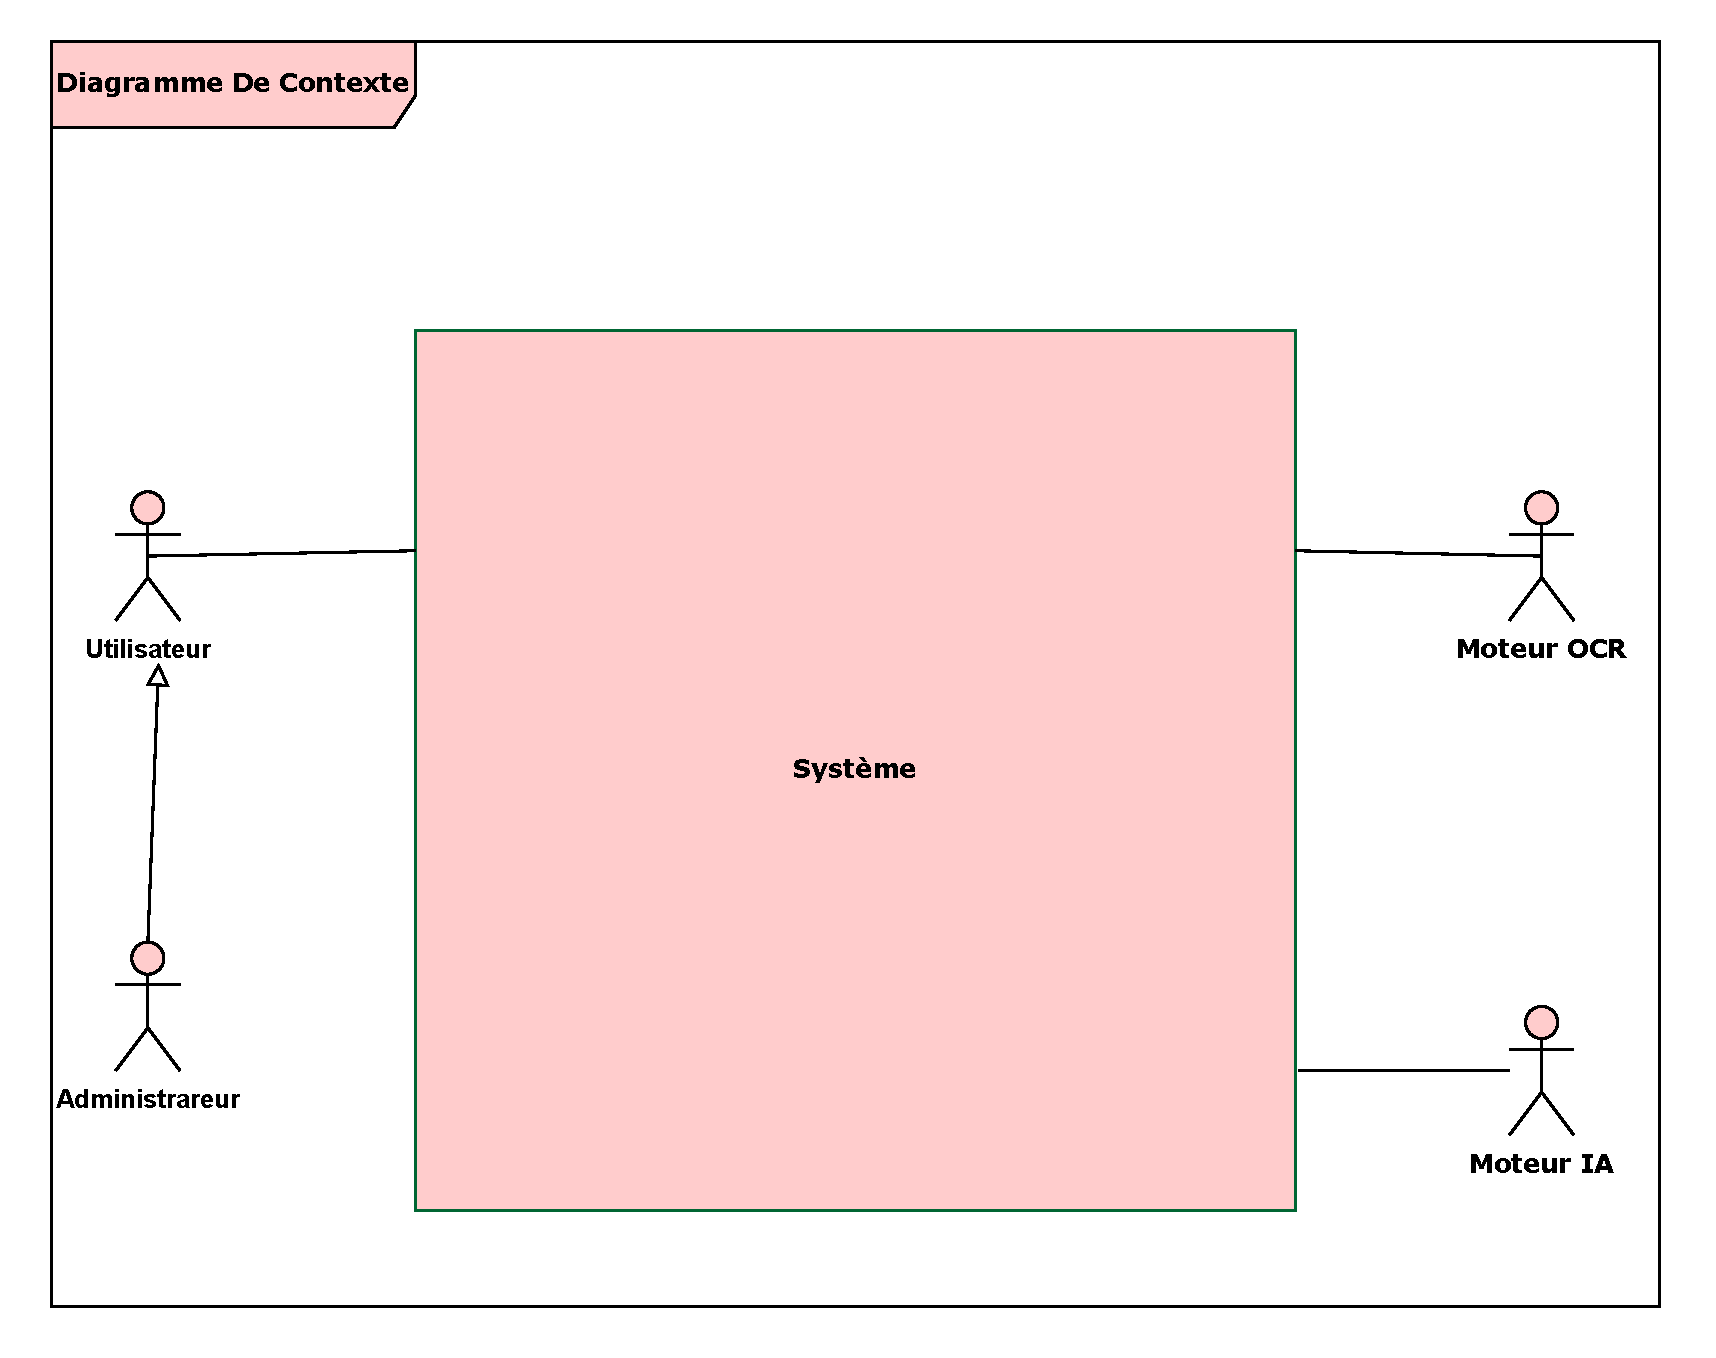
\includegraphics[width=0.9\paperwidth]{chapters/chapter04/diagrammes/DiagrammeDeContexte.pdf}}
    \caption{\itshape Diagramme de contexte du module Ophélia}
    \label{fig:diagramme-contexte}
\end{figure}

\subsection{Diagramme de packages}
\label{subsec:diagramme-package}

Nous avons opté pour une \textbf{décomposition modulaire} afin de garantir une meilleure
maintenabilité, une évolutivité simplifiée et une plus grande flexibilité pour les
développements futurs. Le diagramme de la figure~\ref{fig:diagramme-package} présente les
\textbf{quatre sous-modules} qui composent Ophélia.

\begin{figure}[H]
    \centering
    \makebox[\linewidth][c]{%
        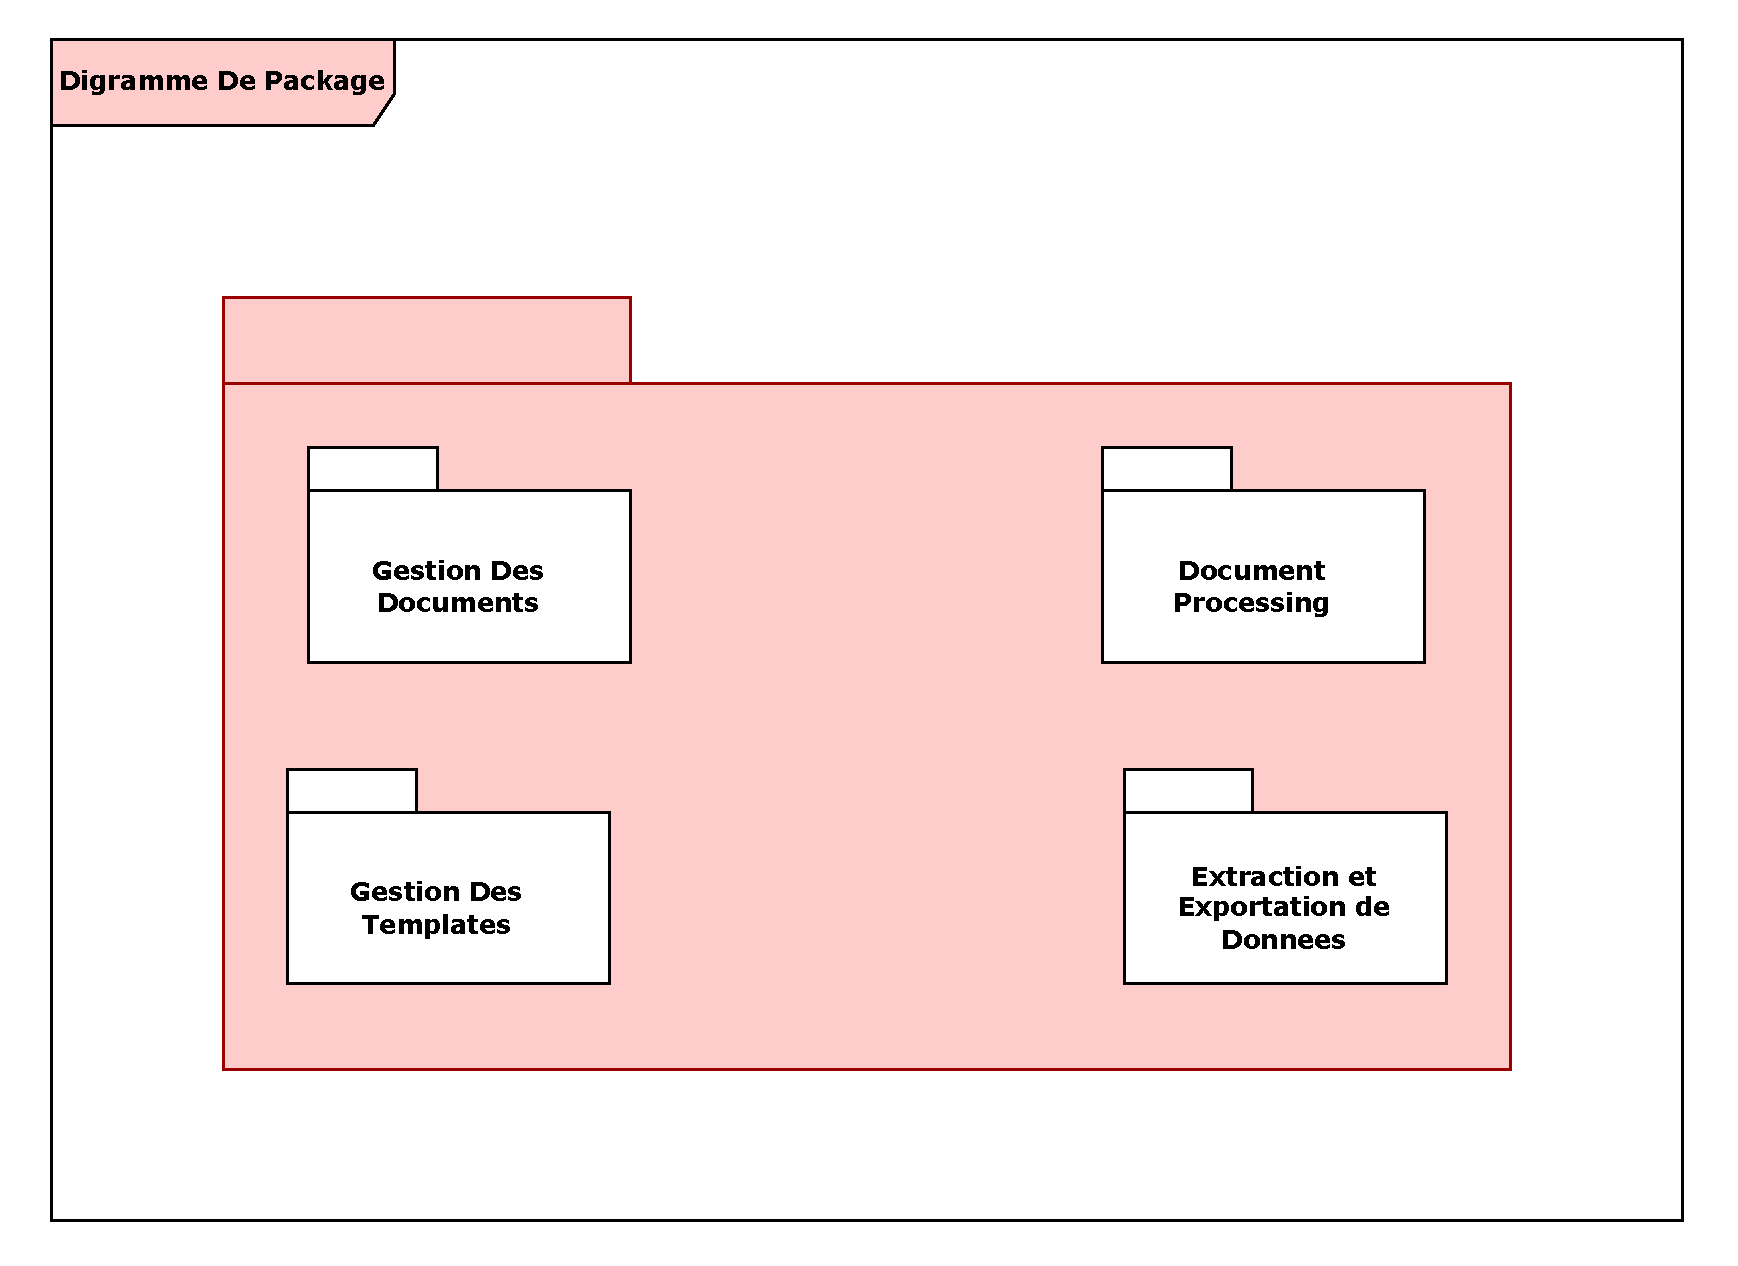
\includegraphics[width=0.9\paperwidth]{chapters/chapter04/diagrammes/DiagrammeDePackage.pdf}}
    \caption{\itshape Diagramme de packages du module Ophélia}
    \label{fig:diagramme-package}
\end{figure}

\begin{itemize}
    \item[\opmanicule] \textbf{Gestion des documents :} sous-module responsable du
    téléversement, de la prévisualisation, de la recherche, du téléchargement et de la
    suppression des documents soumis au module.

    \item[\opmanicule] \textbf{Traitement des documents :} sous-module qui prend en charge la
    détection du type de document, l'extraction du texte, l'analyse de l'agencement,
    l'appariement à un template, la sélection de la stratégie et le calcul des scores de
    confiance.

    \item[\opmanicule] \textbf{Gestion des templates :} sous-module qui permet de créer,
    éditer, tester, versionner et supprimer les templates d'extraction, ainsi que de configurer
    les champs à extraire et leur position relative.

    \item[\opmanicule] \textbf{Extraction et exportation des données :} sous-module chargé de
    l'extraction des données par océrisation ou par intelligence artificielle, de la
    visualisation et de la validation des résultats, puis de leur exportation aux formats XML
    et JSON.
\end{itemize}

\subsection{Diagrammes de cas d'utilisation}
\label{subsec:diagrammes-cas-utilisation}

Pour chacun des sous-modules identifiés au diagramme de packages précédent, nous avons élaboré
un \textbf{diagramme de cas d'utilisation} spécifique. Ces diagrammes représentent
graphiquement les interactions entre les acteurs et les fonctionnalités offertes par le module
\cite{omg2017uml}.

%------------------------------------------------------------------
\subsubsection{Diagramme de cas d'utilisation du package gestion des documents}
%------------------------------------------------------------------

La figure~\ref{fig:uc-gestion-documents} présente le diagramme de cas d'utilisation du package
\textbf{gestion des documents}.

\begin{figure}[H]
    \centering
    \makebox[\linewidth][c]{%
        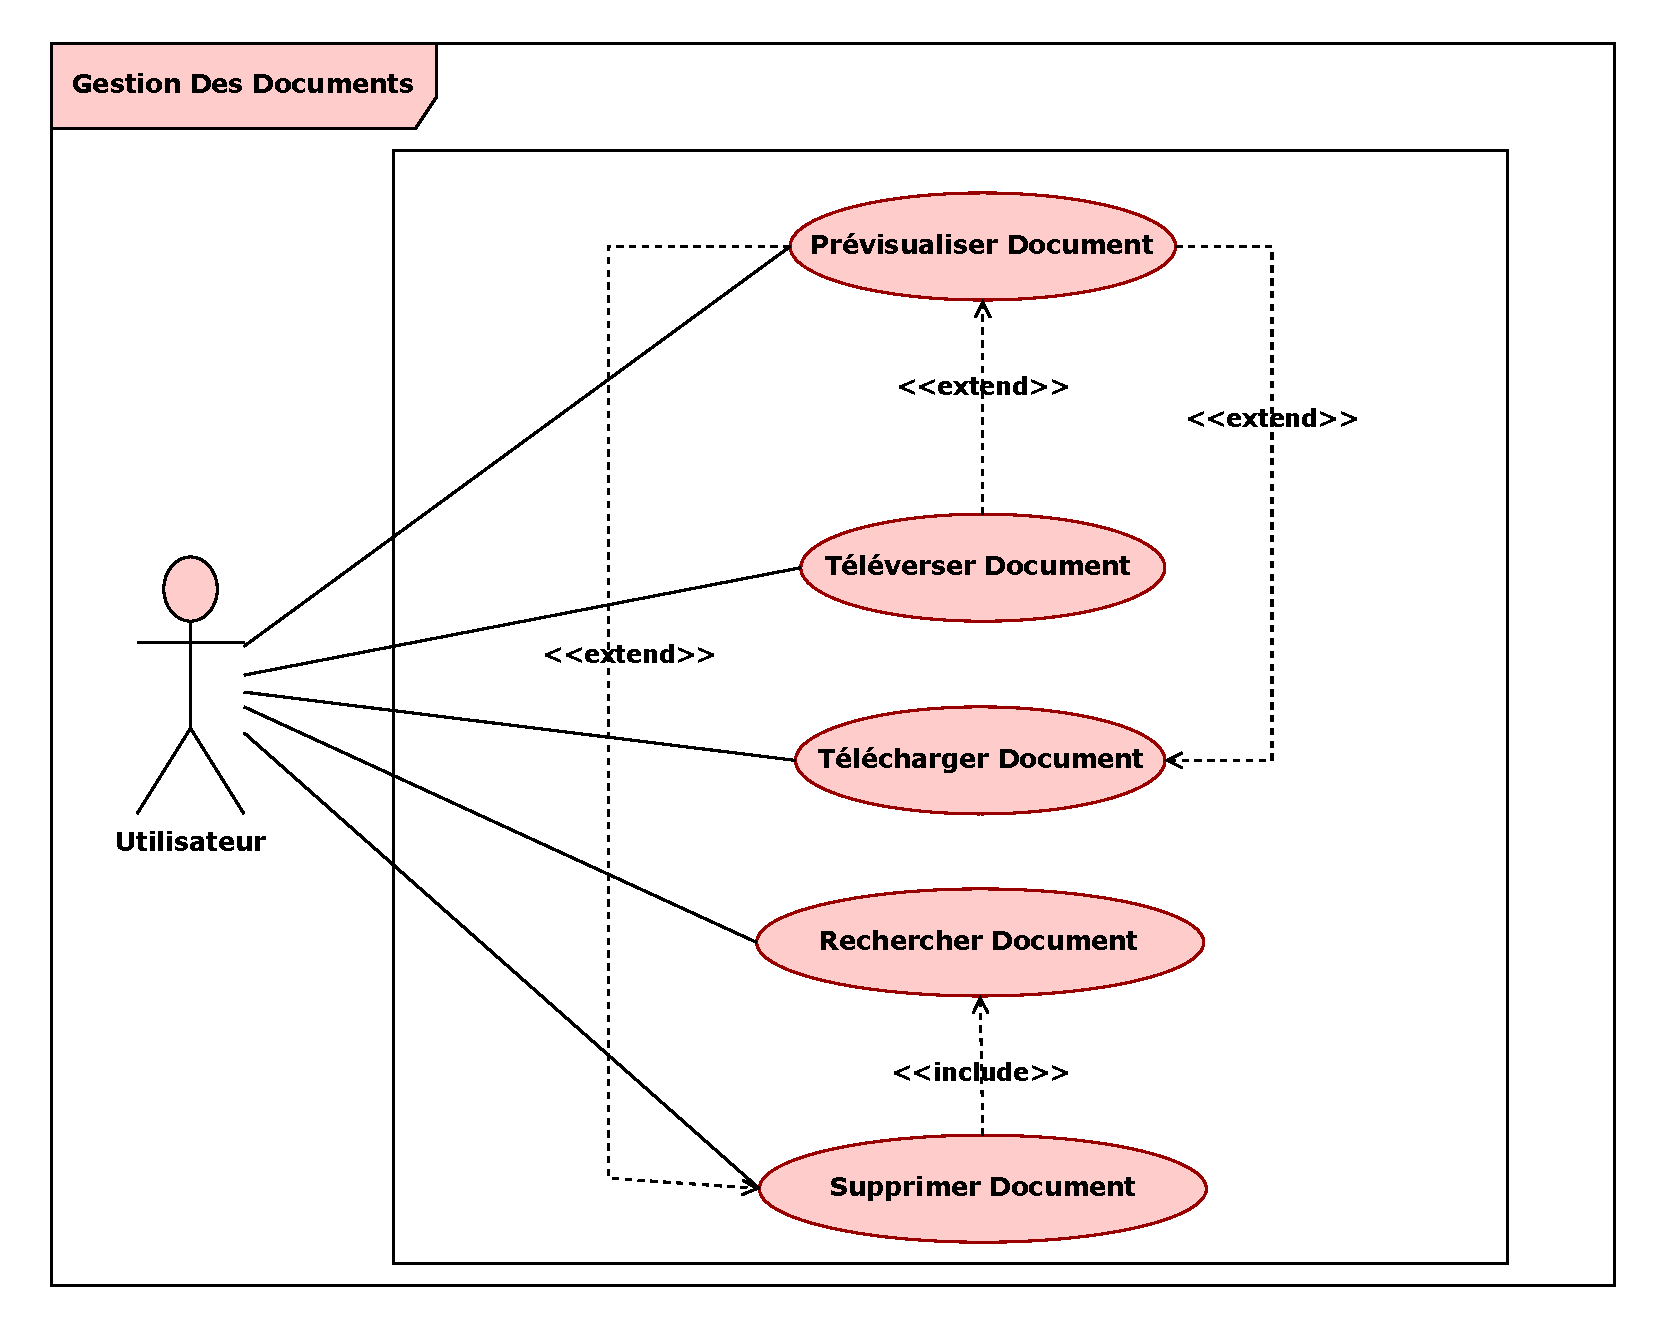
\includegraphics[width=0.9\paperwidth]{chapters/chapter04/diagrammes/DiagrammeUseCaseGestionDocuments.pdf}}
    \caption{\itshape Diagramme de cas d'utilisation du package gestion des documents}
    \label{fig:uc-gestion-documents}
\end{figure}

\noindent\textbf{Description textuelle des cas d'utilisation du package gestion des documents :}

\begin{enumerate}
    \item \textbf{Cas d'utilisation « Téléverser document »}
\end{enumerate}

\begin{table}[H]
    \centering
    \caption{Description textuelle du cas d'utilisation « Téléverser document ».}
    \label{tab:cu-televerser-document}
    \begin{tabularx}{\linewidth}{|p{0.22\linewidth}|X|}
        \hline
        \rowcolor[HTML]{FFCCCC}
        \textbf{Objectif} & Permettre à l'utilisateur d'importer un document dans le module en
        vue de son traitement : extraction, validation, export. \\
        \hline
        \textbf{Acteur primaire} & Utilisateur \\
        \hline
        \textbf{Précondition} & L'utilisateur est authentifié dans Dolibarr et dispose du
        droit de téléversement déclaré par le module. \\
        \hline
        \textbf{Postcondition} & Le document est enregistré et devient disponible pour le
        traitement. \\
        \hline
        \textbf{Scénario nominal} &
        1. L'utilisateur sélectionne l'option « Téléverser un document ». \newline
        2. Le module affiche une interface de sélection de fichier. \newline
        3. L'utilisateur choisit un fichier depuis son poste, au format PDF ou image. \newline
        4. Le module vérifie le format et la taille du fichier. \newline
        5. Le module enregistre le document et l'associe à l'utilisateur. \newline
        6. Le module confirme le succès du téléversement. \\
        \hline
        \textbf{Scénario alternatif} &
        4a. Format non supporté $\rightarrow$ message d'erreur, retour à l'étape 3. \newline
        4b. Fichier trop volumineux $\rightarrow$ message d'erreur, retour à l'étape 3. \\
        \hline
        \textbf{Relation} & \opstereo{extend} vers « Prévisualiser document » : une
        prévisualisation peut être proposée immédiatement après le téléversement. \\
        \hline
    \end{tabularx}
\end{table}

\begin{enumerate}
    \setcounter{enumi}{1}
    \item \textbf{Cas d'utilisation « Rechercher document »}
\end{enumerate}

\begin{table}[H]
    \centering
    \caption{Description textuelle du cas d'utilisation « Rechercher document ».}
    \label{tab:cu-rechercher-document}
    \begin{tabularx}{\linewidth}{|p{0.22\linewidth}|X|}
        \hline
        \rowcolor[HTML]{FFCCCC}
        \textbf{Objectif} & Permettre à l'utilisateur de retrouver un ou plusieurs documents à
        partir de critères de recherche. \\
        \hline
        \textbf{Acteur primaire} & Utilisateur \\
        \hline
        \textbf{Précondition} & Au moins un document existe dans le module. \\
        \hline
        \textbf{Postcondition} & Une liste de documents correspondant aux critères est affichée
        à l'utilisateur. \\
        \hline
        \textbf{Scénario nominal} &
        1. L'utilisateur accède à la fonctionnalité de recherche. \newline
        2. L'utilisateur saisit un ou plusieurs critères : nom, type, date, mot-clé,
        statut. \newline
        3. Le module interroge la base documentaire. \newline
        4. Le module affiche la liste des résultats correspondants. \newline
        5. L'utilisateur sélectionne un document pour une action complémentaire :
        prévisualisation, téléchargement ou suppression. \\
        \hline
        \textbf{Scénario alternatif} &
        4a. Aucun résultat trouvé $\rightarrow$ le module affiche « Aucun document
        trouvé ». \\
        \hline
        \textbf{Relation} & « Supprimer document » \opstereo{include} « Rechercher document » :
        l'utilisateur doit localiser un document avant de pouvoir le supprimer. \\
        \hline
    \end{tabularx}
\end{table}

%------------------------------------------------------------------
\subsubsection{Diagramme de cas d'utilisation du package gestion des templates}
%------------------------------------------------------------------

La figure~\ref{fig:uc-gestion-templates} présente le diagramme de cas d'utilisation du package
\textbf{gestion des templates}.

\begin{figure}[H]
    \centering
    \makebox[\linewidth][c]{%
        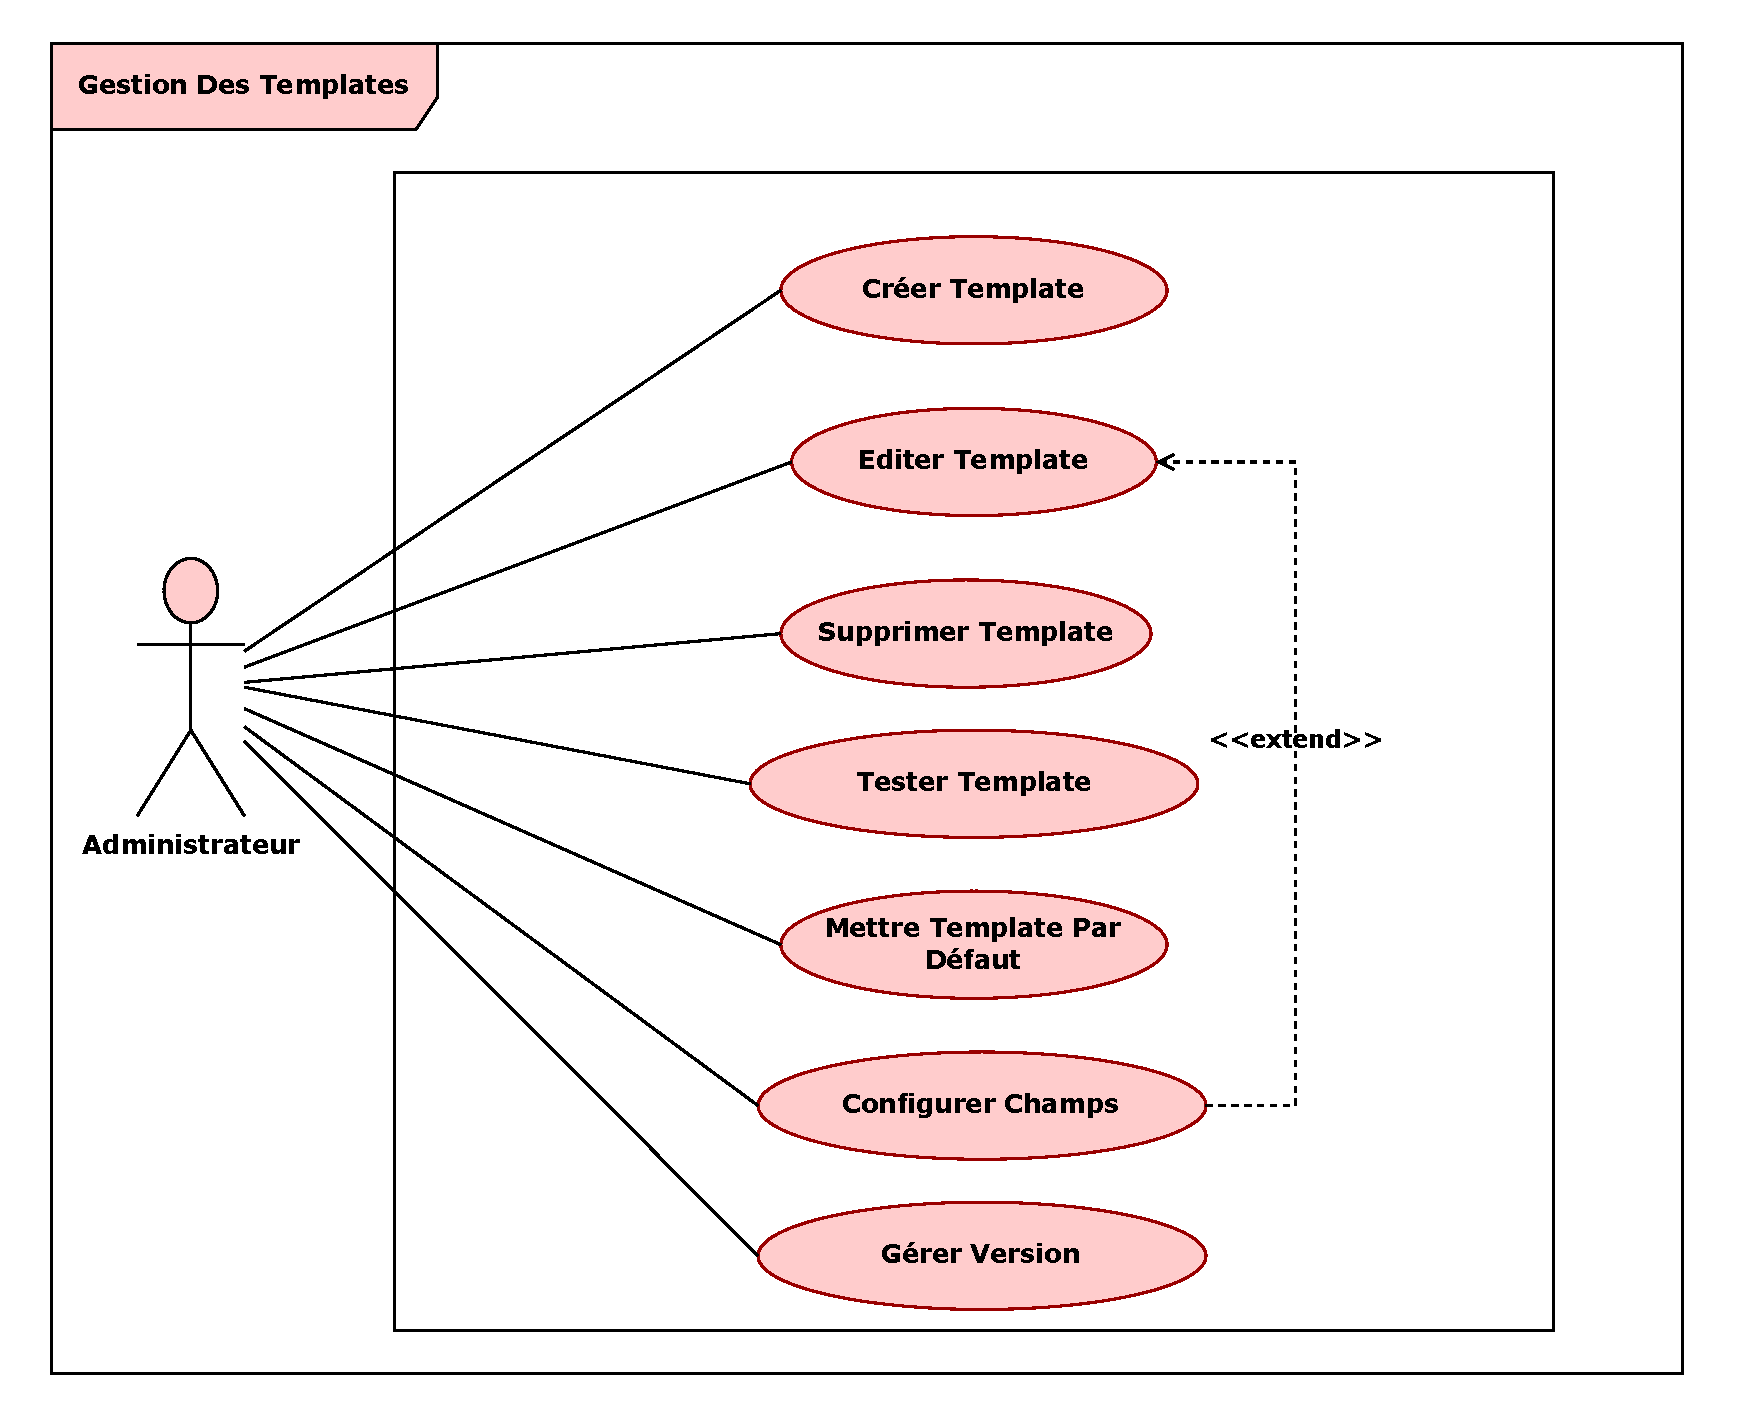
\includegraphics[width=0.9\paperwidth]{chapters/chapter04/diagrammes/DiagrammeUseCaseGestionTemplates.drawio.pdf}}
    \caption{\itshape Diagramme de cas d'utilisation du package gestion des templates}
    \label{fig:uc-gestion-templates}
\end{figure}

\noindent\textbf{Description textuelle des cas d'utilisation du package gestion des templates :}

\begin{enumerate}
    \item \textbf{Cas d'utilisation « Créer template »}
\end{enumerate}

\begin{table}[H]
    \centering
    \caption{Description textuelle du cas d'utilisation « Créer template ».}
    \label{tab:cu-creer-template}
    \begin{tabularx}{\linewidth}{|p{0.22\linewidth}|X|}
        \hline
        \rowcolor[HTML]{FFCCCC}
        \textbf{Objectif} & Définir un nouveau template décrivant la structure attendue d'un
        type de document et les champs à en extraire, par sélection interactive des zones
        d'intérêt sur un document déjà traité. \\
        \hline
        \textbf{Acteur primaire} & Administrateur \\
        \hline
        \textbf{Précondition} & L'administrateur dispose du droit de gestion des templates et
        un document océrisé est disponible comme document de référence. \\
        \hline
        \textbf{Postcondition} & Un nouveau template est enregistré et disponible pour
        l'appariement avec des documents ultérieurs. \\
        \hline
        \textbf{Scénario nominal} &
        1. L'administrateur sélectionne un document traité comme référence et choisit « Créer
        un template ». \newline
        2. Le module récupère les éléments textuels océrisés du document et les affiche en
        superposition. \newline
        3. L'administrateur renseigne les informations générales du template : nom, type de
        document associé, description. \newline
        4. L'administrateur délimite les zones repères qui serviront d'ancres à
        l'appariement. \newline
        5. Le module enregistre la position relative de chaque zone et vérifie la cohérence de
        la saisie. \newline
        6. Le module enregistre le nouveau template. \\
        \hline
        \textbf{Scénario alternatif} &
        2a. Le document de référence n'a pas été océrisé $\rightarrow$ le module déclenche
        d'abord son traitement. \newline
        5a. Informations obligatoires manquantes ou incohérentes $\rightarrow$ message
        d'erreur, retour à l'étape 3. \newline
        5b. Un template similaire existe déjà $\rightarrow$ le module propose de le dupliquer
        ou de le modifier plutôt que d'en créer un nouveau. \\
        \hline
        \textbf{Relation} & \opstereo{include} « Configurer champs » : la définition des champs
        à extraire fait partie intégrante de la création d'un template. \\
        \hline
    \end{tabularx}
\end{table}

\begin{enumerate}
    \setcounter{enumi}{1}
    \item \textbf{Cas d'utilisation « Configurer champs »}
\end{enumerate}

\begin{table}[H]
    \centering
    \caption{Description textuelle du cas d'utilisation « Configurer champs ».}
    \label{tab:cu-configurer-champs}
    \begin{tabularx}{\linewidth}{|p{0.22\linewidth}|X|}
        \hline
        \rowcolor[HTML]{FFCCCC}
        \textbf{Objectif} & Paramétrer les champs de données à extraire pour un template
        donné : libellé, type, texte de la clé, position relative de la valeur et règles de
        validation. \\
        \hline
        \textbf{Acteur primaire} & Administrateur \\
        \hline
        \textbf{Précondition} & Un template existe préalablement, créé via le cas d'utilisation
        « Créer template ». \\
        \hline
        \textbf{Postcondition} & La configuration des champs du template est enregistrée et
        utilisable pour l'extraction. \\
        \hline
        \textbf{Scénario nominal} &
        1. L'administrateur sélectionne un template existant. \newline
        2. L'administrateur accède à la section « Configurer les champs ». \newline
        3. L'administrateur ajoute, modifie ou supprime un champ en désignant sur le document
        la zone de la clé puis celle de la valeur. \newline
        4. Le module enregistre la position de la valeur relativement à sa clé et en déduit le
        sens de la relation. \newline
        5. Le module vérifie la cohérence de la configuration : absence de doublon, types
        valides, zones non chevauchantes. \newline
        6. Le module enregistre la configuration des champs. \\
        \hline
        \textbf{Scénario alternatif} &
        5a. Configuration incohérente, par exemple une zone chevauchant celle d'un autre champ
        $\rightarrow$ message d'erreur, retour à l'étape 3. \\
        \hline
        \textbf{Relation} & \opstereo{include} de « Créer template » et \opstereo{extend} de
        « Éditer template » : la configuration des champs est requise à la création et peut
        être reprise lors d'une édition ultérieure. \\
        \hline
    \end{tabularx}
\end{table}

%------------------------------------------------------------------
\subsubsection{Diagramme de cas d'utilisation du package traitement des documents}
%------------------------------------------------------------------

La figure~\ref{fig:uc-traitement-documents} présente le diagramme de cas d'utilisation du
package \textbf{traitement des documents}.

\begin{figure}[H]
    \centering
    \makebox[\linewidth][c]{%
        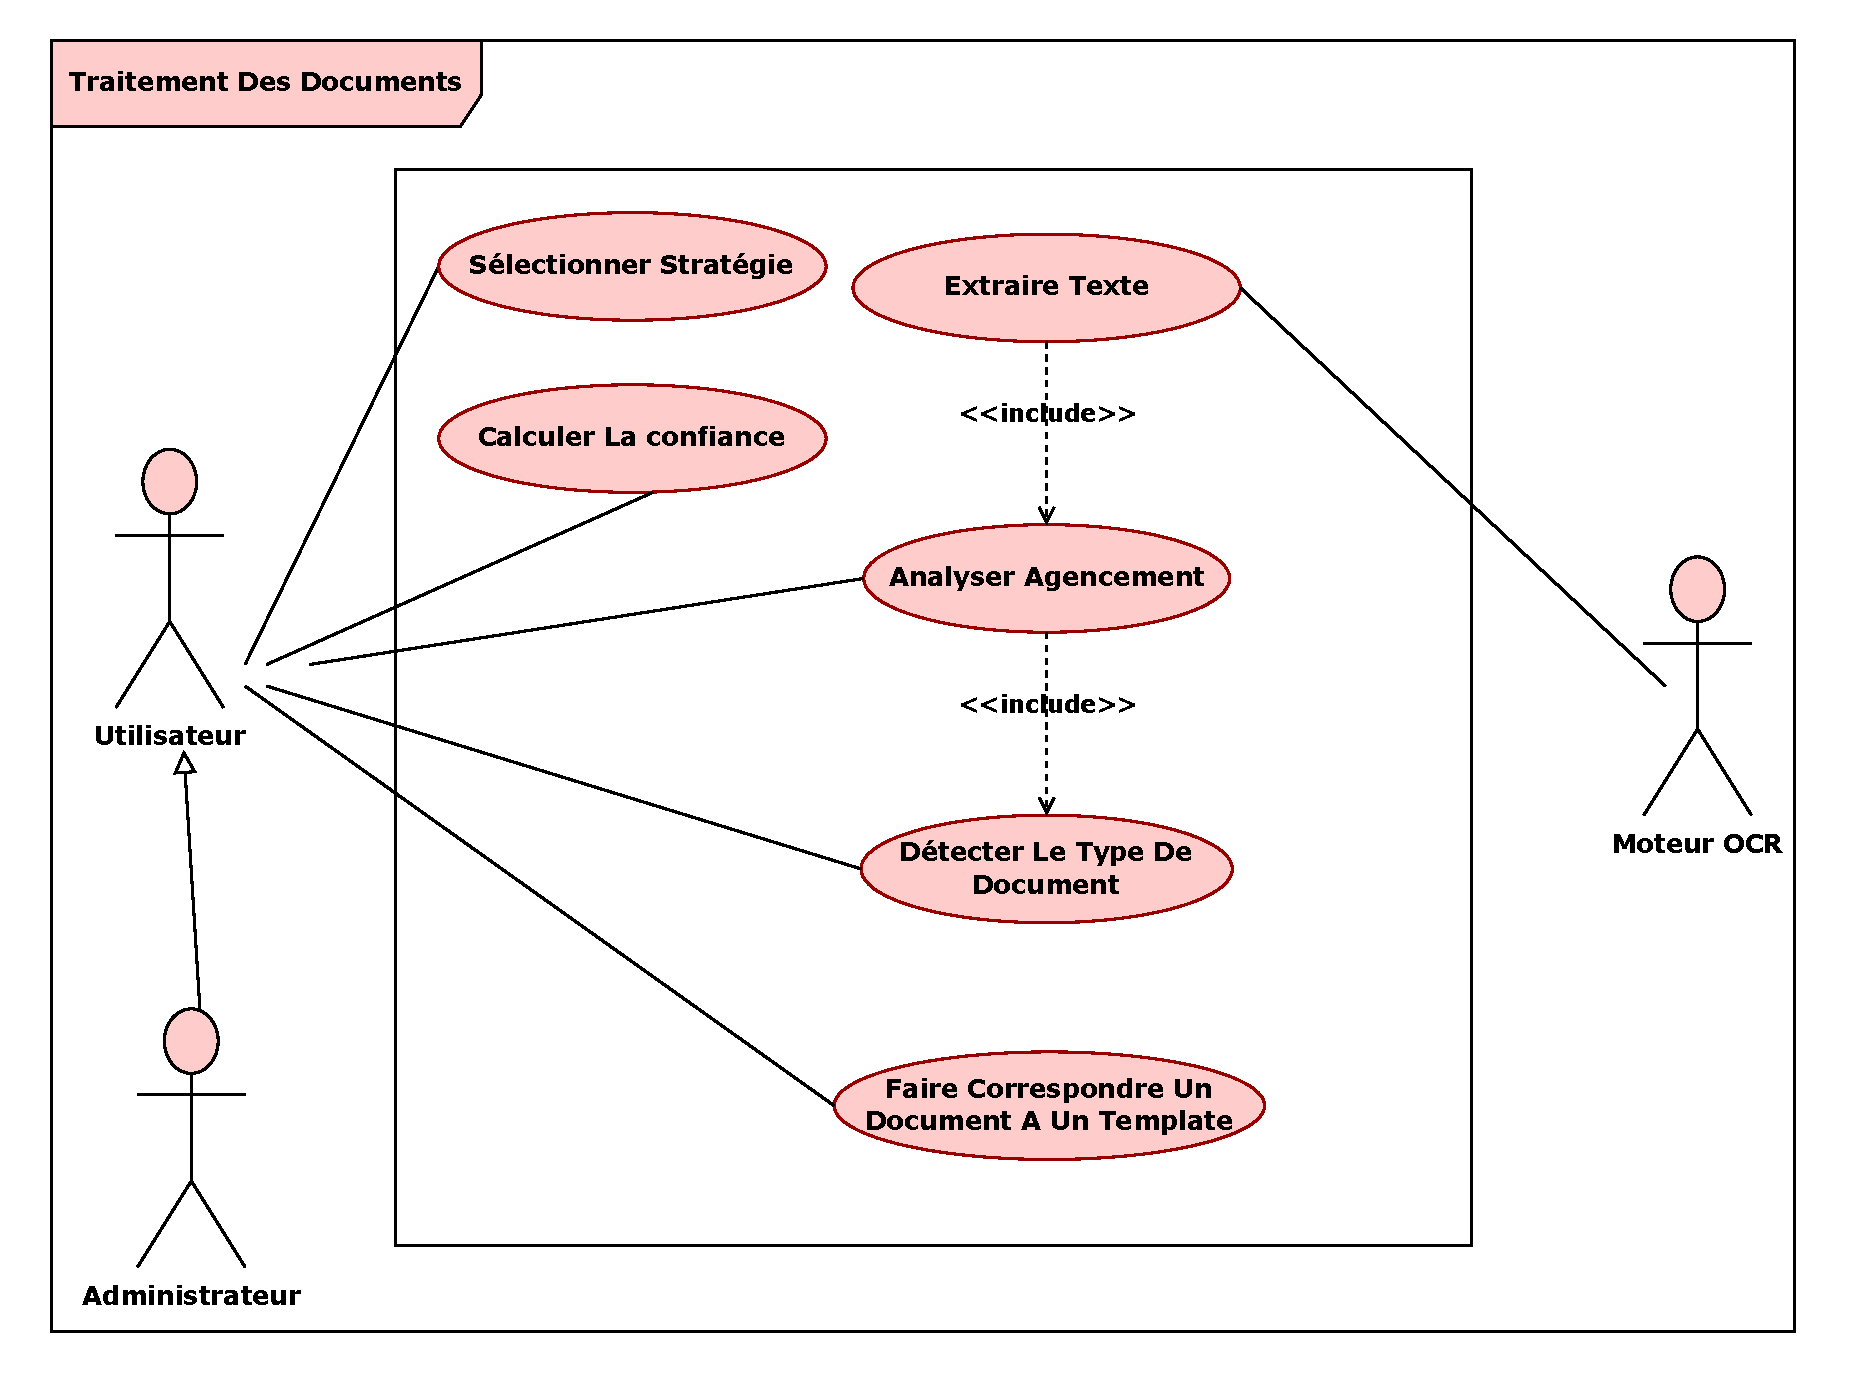
\includegraphics[width=0.9\paperwidth]{chapters/chapter04/diagrammes/DiagrammeUseCaseTraitementDesDocuments.pdf}}
    \caption{\itshape Diagramme de cas d'utilisation du package traitement des documents}
    \label{fig:uc-traitement-documents}
\end{figure}

\noindent\textbf{Description textuelle des cas d'utilisation du package traitement des documents :}

\begin{enumerate}
    \item \textbf{Cas d'utilisation « Faire correspondre un document à un template »}
\end{enumerate}

\begin{table}[H]
    \centering
    \caption{Description textuelle du cas d'utilisation « Faire correspondre un document à un
    template ».}
    \label{tab:cu-correspondance-template}
    \begin{tabularx}{\linewidth}{|p{0.22\linewidth}|X|}
        \hline
        \rowcolor[HTML]{FFCCCC}
        \textbf{Objectif} & Identifier le template le plus adapté à un document donné, à partir
        du type détecté et de l'agencement analysé. \\
        \hline
        \textbf{Acteur primaire} & Utilisateur \\
        \hline
        \textbf{Précondition} & Le document a été téléversé, son type a été détecté et son
        agencement analysé ; des templates existent dans le module. \\
        \hline
        \textbf{Postcondition} & Le document est associé à un template, assorti d'un score de
        correspondance. \\
        \hline
        \textbf{Scénario nominal} &
        1. L'utilisateur lance le traitement du document. \newline
        2. Le module récupère le type détecté et le résultat de l'analyse d'agencement. \newline
        3. Le module évalue le degré de correspondance de chaque template candidat. \newline
        4. Le module sélectionne le template le mieux noté. \newline
        5. Le module associe le document au template retenu et affiche le score obtenu. \\
        \hline
        \textbf{Scénario alternatif} &
        4a. Aucun template n'atteint le seuil de décision $\rightarrow$ le document est marqué
        « non reconnu » et signalé à l'administrateur, qui peut créer un nouveau template ou
        effectuer une association manuelle ; le module bascule par défaut vers la stratégie
        d'extraction par intelligence artificielle. \\
        \hline
        \textbf{Relation} & \opstereo{include} de « Extraire les données » : l'appariement
        constitue une étape obligatoire du traitement déclenché par l'utilisateur. \\
        \hline
    \end{tabularx}
\end{table}

\begin{enumerate}
    \setcounter{enumi}{1}
    \item \textbf{Cas d'utilisation « Sélectionner stratégie »}
\end{enumerate}

\begin{table}[H]
    \centering
    \caption{Description textuelle du cas d'utilisation « Sélectionner stratégie ».}
    \label{tab:cu-selectionner-strategie}
    \begin{tabularx}{\linewidth}{|p{0.22\linewidth}|X|}
        \hline
        \rowcolor[HTML]{FFCCCC}
        \textbf{Objectif} & Choisir la stratégie de traitement appliquée au document pour
        l'extraction des données : appariement de templates, océrisation, intelligence
        artificielle ou approche combinée. \\
        \hline
        \textbf{Acteur primaire} & Utilisateur ; Administrateur en mode supervisé \\
        \hline
        \textbf{Précondition} & Un document est en cours de traitement et plusieurs stratégies
        sont disponibles dans le module. \\
        \hline
        \textbf{Postcondition} & Une stratégie de traitement est sélectionnée et appliquée au
        pipeline d'extraction du document. \\
        \hline
        \textbf{Scénario nominal} &
        1. L'utilisateur lance le traitement du document. \newline
        2. Le module évalue les caractéristiques du document : type, qualité d'océrisation,
        degré de correspondance obtenu. \newline
        3. Le module applique la stratégie dont les conditions d'activation sont
        satisfaites. \newline
        4. Le module configure le pipeline de traitement en conséquence et en informe
        l'utilisateur. \\
        \hline
        \textbf{Scénario alternatif} &
        3a. Mode supervisé activé $\rightarrow$ le module propose les stratégies compatibles et
        l'administrateur sélectionne celle à appliquer. \newline
        3b. La stratégie retenue produit une confiance insuffisante $\rightarrow$ le module
        bascule automatiquement vers la stratégie de repli. \\
        \hline
        \textbf{Relation} & \opstereo{include} de « Extraire les données » : la sélection de la
        stratégie précède nécessairement l'extraction. \\
        \hline
    \end{tabularx}
\end{table}

%------------------------------------------------------------------
\subsubsection{Diagramme de cas d'utilisation du package extraction et exportation des données}
%------------------------------------------------------------------

La figure~\ref{fig:uc-extraction-exportation} présente le diagramme de cas d'utilisation du
package \textbf{extraction, validation et exportation} des données.

\begin{figure}[H]
    \centering
    \makebox[\linewidth][c]{%
        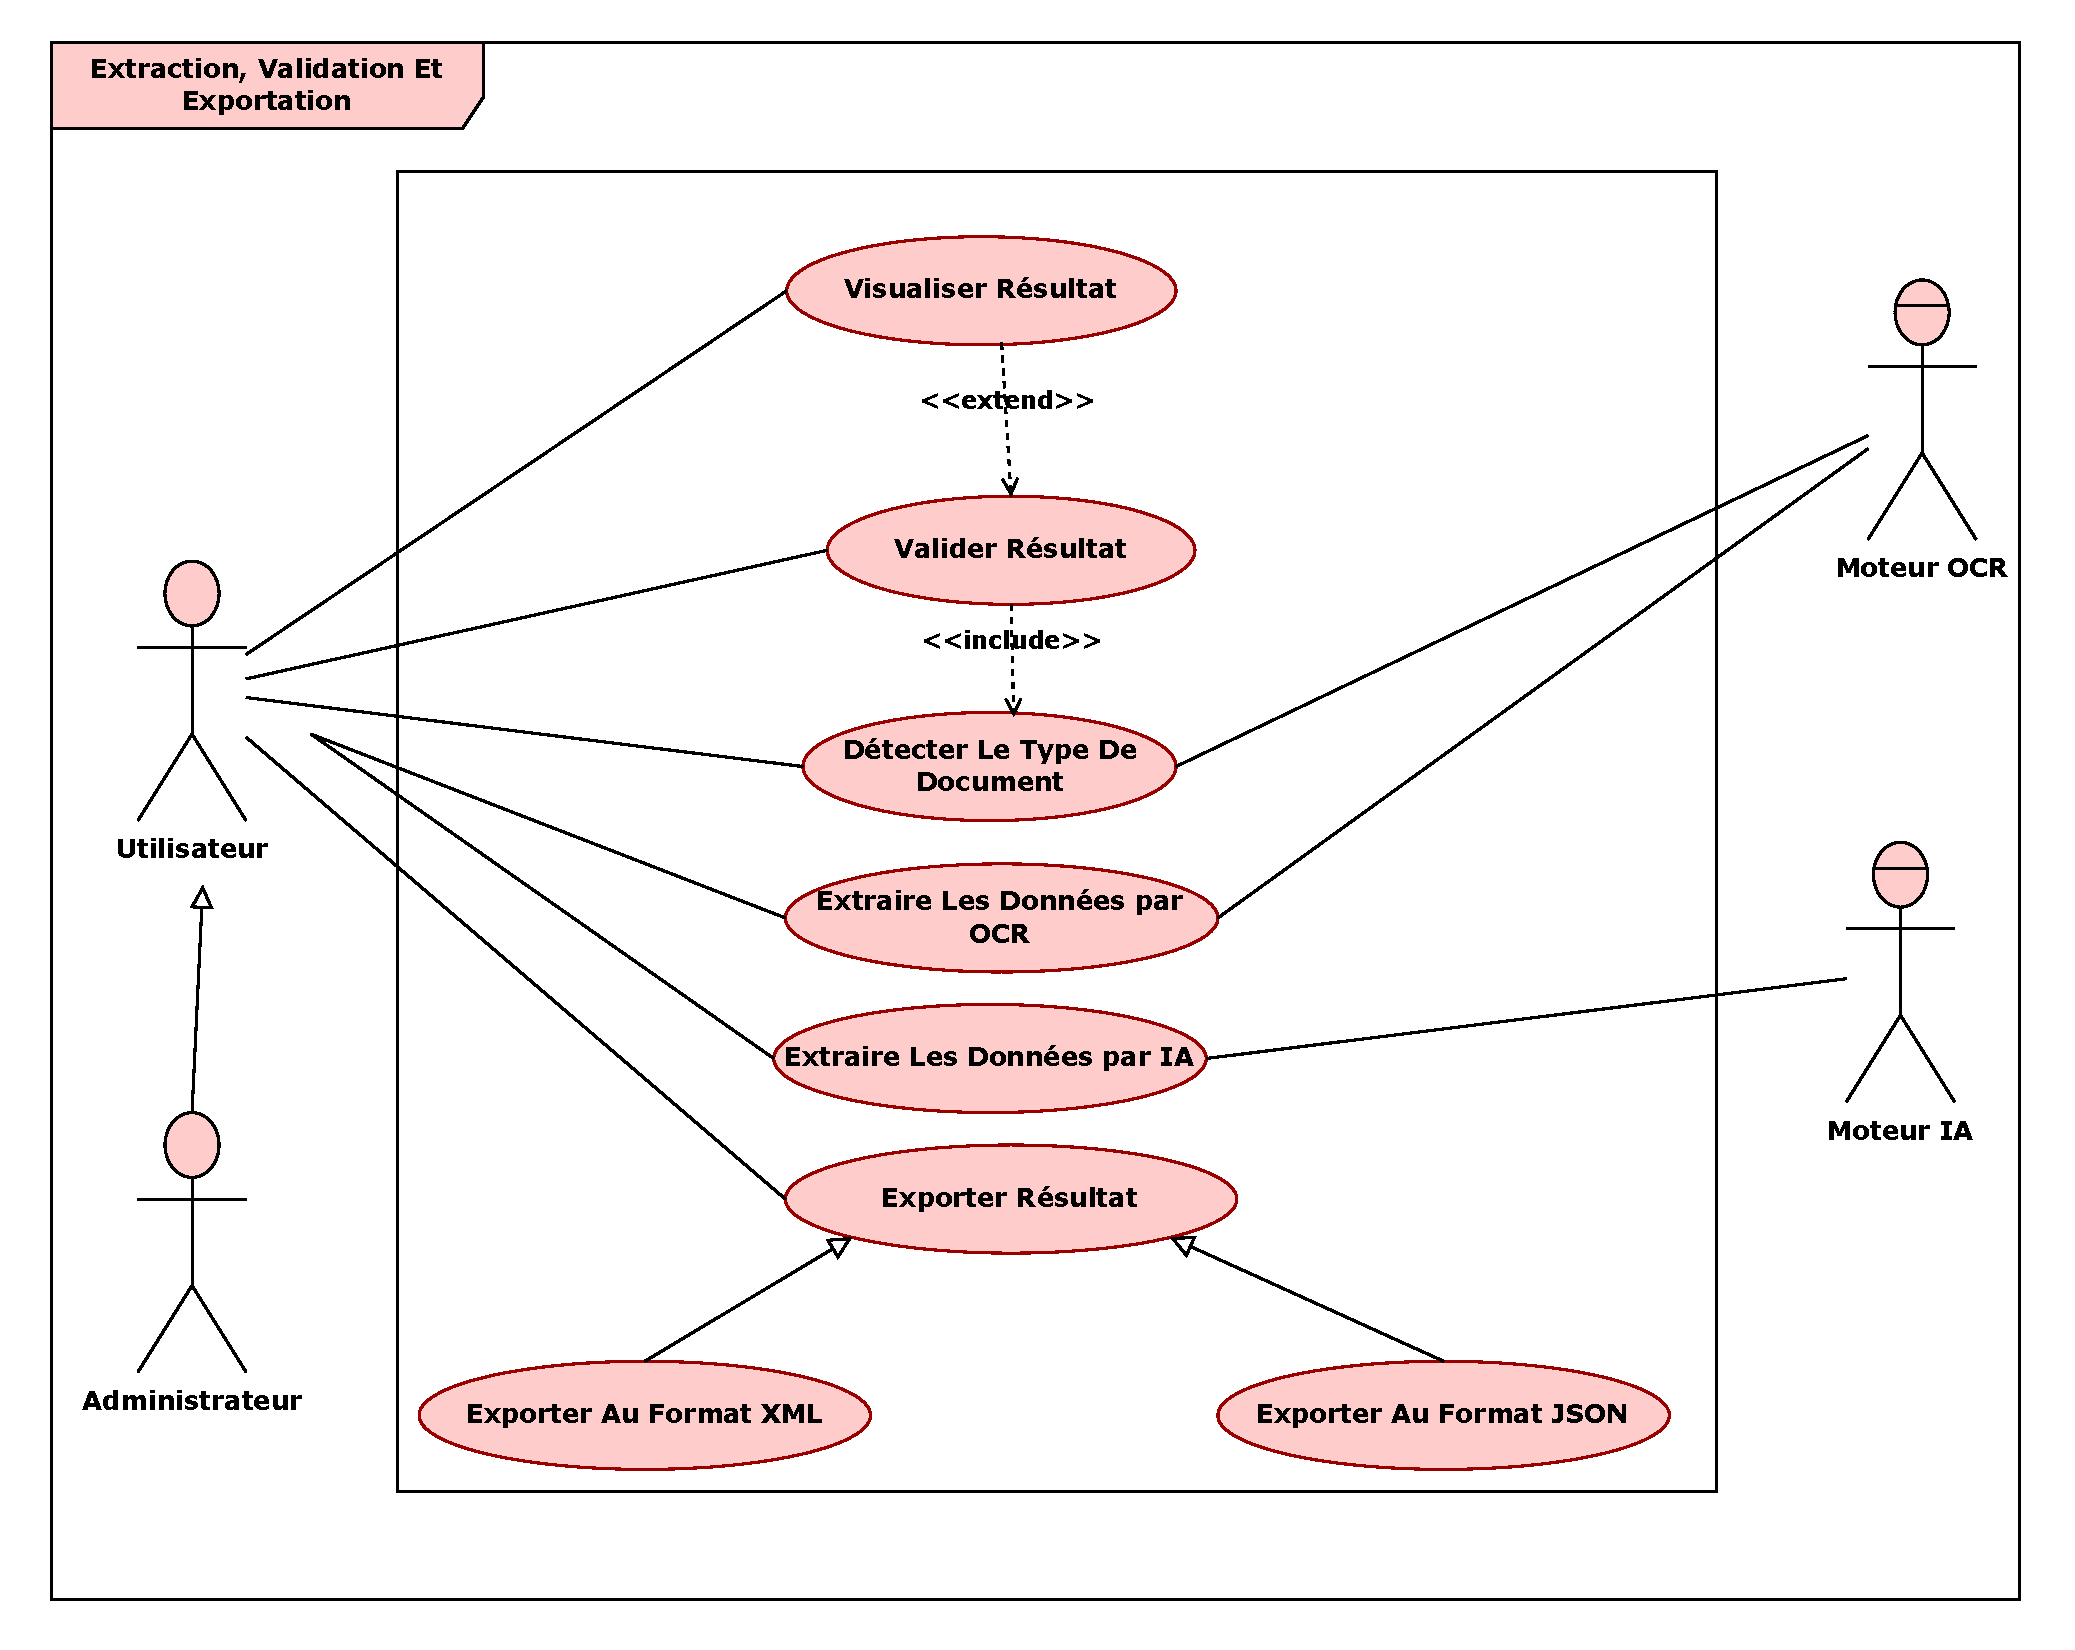
\includegraphics[width=0.9\paperwidth]{chapters/chapter04/diagrammes/DiagrammeUseCaseExtractionDesDonees.pdf}}
    \caption{\itshape Diagramme de cas d'utilisation du package extraction, validation et exportation}
    \label{fig:uc-extraction-exportation}
\end{figure}

\noindent\textbf{Description textuelle des cas d'utilisation du package extraction, validation et exportation :}

\begin{enumerate}
    \item \textbf{Cas d'utilisation « Visualiser résultat »}
\end{enumerate}

\begin{table}[H]
    \centering
    \caption{Description textuelle du cas d'utilisation « Visualiser résultat ».}
    \label{tab:cu-visualiser-resultat}
    \begin{tabularx}{\linewidth}{|p{0.22\linewidth}|X|}
        \hline
        \rowcolor[HTML]{FFCCCC}
        \textbf{Objectif} & Afficher les données extraites d'un document afin de les consulter
        avant leur validation ou leur export. \\
        \hline
        \textbf{Acteur primaire} & Utilisateur \\
        \hline
        \textbf{Précondition} & Une extraction, par appariement de template, par océrisation ou
        par intelligence artificielle, a été effectuée sur le document. \\
        \hline
        \textbf{Postcondition} & Les résultats d'extraction sont affichés à l'utilisateur. \\
        \hline
        \textbf{Scénario nominal} &
        1. L'utilisateur sélectionne un document traité. \newline
        2. L'utilisateur accède à la vue « Résultat d'extraction ». \newline
        3. Le module affiche les champs extraits avec leurs valeurs et leur niveau de
        confiance. \newline
        4. L'utilisateur navigue entre le document original et les données extraites. \\
        \hline
        \textbf{Scénario alternatif} &
        3a. Extraction incomplète ou en échec sur certains champs $\rightarrow$ ces champs sont
        signalés visuellement afin d'attirer l'attention de l'utilisateur. \\
        \hline
        \textbf{Relation} & \opstereo{extend} vers « Valider résultat » : la visualisation peut
        mener directement à une action de validation. \\
        \hline
    \end{tabularx}
\end{table}

\begin{enumerate}
    \setcounter{enumi}{1}
    \item \textbf{Cas d'utilisation « Valider résultat »}
\end{enumerate}

\begin{table}[H]
    \centering
    \caption{Description textuelle du cas d'utilisation « Valider résultat ».}
    \label{tab:cu-valider-resultat}
    \begin{tabularx}{\linewidth}{|p{0.22\linewidth}|X|}
        \hline
        \rowcolor[HTML]{FFCCCC}
        \textbf{Objectif} & Contrôler champ par champ les valeurs proposées par le module,
        corriger celles qui sont erronées, et marquer le résultat d'extraction comme validé. \\
        \hline
        \textbf{Acteur primaire} & Utilisateur \\
        \hline
        \textbf{Précondition} & Un résultat d'extraction non encore validé est disponible pour
        le document concerné. \\
        \hline
        \textbf{Postcondition} & Le résultat d'extraction est marqué comme validé, les
        corrections sont enregistrées et le template associé est réajusté en conséquence. \\
        \hline
        \textbf{Scénario nominal} &
        1. L'utilisateur accède au résultat d'extraction d'un document traité. \newline
        2. Le module présente les champs par niveau de confiance croissant, afin de placer en
        tête ceux qui appellent une vérification. \newline
        3. L'utilisateur confirme les valeurs correctes. \newline
        4. L'utilisateur corrige les valeurs erronées en désignant la zone exacte sur le
        document. \newline
        5. Le module enregistre chaque correction et met à jour la position de référence du
        champ dans le template concerné. \newline
        6. L'utilisateur valide l'ensemble du résultat. \newline
        7. Le module marque le document comme validé et l'autorise à l'export. \\
        \hline
        \textbf{Scénario alternatif} &
        4a. Un champ obligatoire est absent du document $\rightarrow$ l'utilisateur le marque
        « non applicable » et le module l'exclut du calcul de complétude. \newline
        6a. L'utilisateur interrompt la validation $\rightarrow$ les corrections déjà saisies
        sont conservées et le document reste à l'état « en cours de validation ». \\
        \hline
        \textbf{Relation} & \opstereo{extend} de « Visualiser résultat » ; constitue un
        prérequis de « Exporter résultat ». Déclenche le réajustement du template. \\
        \hline
    \end{tabularx}
\end{table}

\begin{enumerate}
    \setcounter{enumi}{2}
    \item \textbf{Cas d'utilisation « Exporter résultat »}
\end{enumerate}

\begin{table}[H]
    \centering
    \caption{Description textuelle du cas d'utilisation « Exporter résultat ».}
    \label{tab:cu-exporter-resultat}
    \begin{tabularx}{\linewidth}{|p{0.22\linewidth}|X|}
        \hline
        \rowcolor[HTML]{FFCCCC}
        \textbf{Objectif} & Exporter les données extraites et validées d'un document sous forme
        d'un fichier structuré téléchargeable. \\
        \hline
        \textbf{Acteur primaire} & Utilisateur ; Administrateur \\
        \hline
        \textbf{Précondition} & Un résultat d'extraction validé est disponible pour le document
        concerné. \\
        \hline
        \textbf{Postcondition} & Un fichier exporté est généré et mis à disposition de
        l'utilisateur en téléchargement. \\
        \hline
        \textbf{Scénario nominal} &
        1. L'utilisateur sélectionne le document ou le résultat à exporter. \newline
        2. L'utilisateur choisit le format d'export souhaité : JSON ou XML. \newline
        3. Le module génère le fichier dans le format sélectionné. \newline
        4. Le module met le fichier à disposition pour téléchargement et journalise
        l'opération. \\
        \hline
        \textbf{Scénario alternatif} &
        1a. Résultat non encore validé $\rightarrow$ l'export est refusé et l'utilisateur est
        redirigé vers « Valider résultat ». \\
        \hline
        \textbf{Relation} & « Exporter au format XML » et « Exporter au format JSON » sont des
        spécialisations de « Exporter résultat ». \\
        \hline
    \end{tabularx}
\end{table}

\subsection{Diagramme de classes}
\label{subsec:diagramme-classes}

Le \textbf{diagramme de classes} (figure~\ref{fig:diagramme-classes}) formalise l'ontologie du
domaine : il présente les entités manipulées par le module, leurs attributs, leurs opérations
ainsi que les relations qui les lient. Il constitue la traduction, en termes orientés objet,
des structures introduites en section~\ref{sec:modelisation-mathematique} : la classe
\textbf{Document} porte la décomposition du document en pages et en éléments textuels
localisés, la classe \textbf{Template} regroupe le type de document, ses champs et ses
métadonnées, la classe \textbf{TemplateField} décrit un champ à extraire, et la classe
\textbf{SpatialVector} matérialise la position d'une valeur relativement à sa clé. Les
énumérations reprennent quant à elles les types de documents pris en charge et les types de
relation spatiale.

\begin{figure}[H]
    \centering
    \makebox[\linewidth][c]{%
        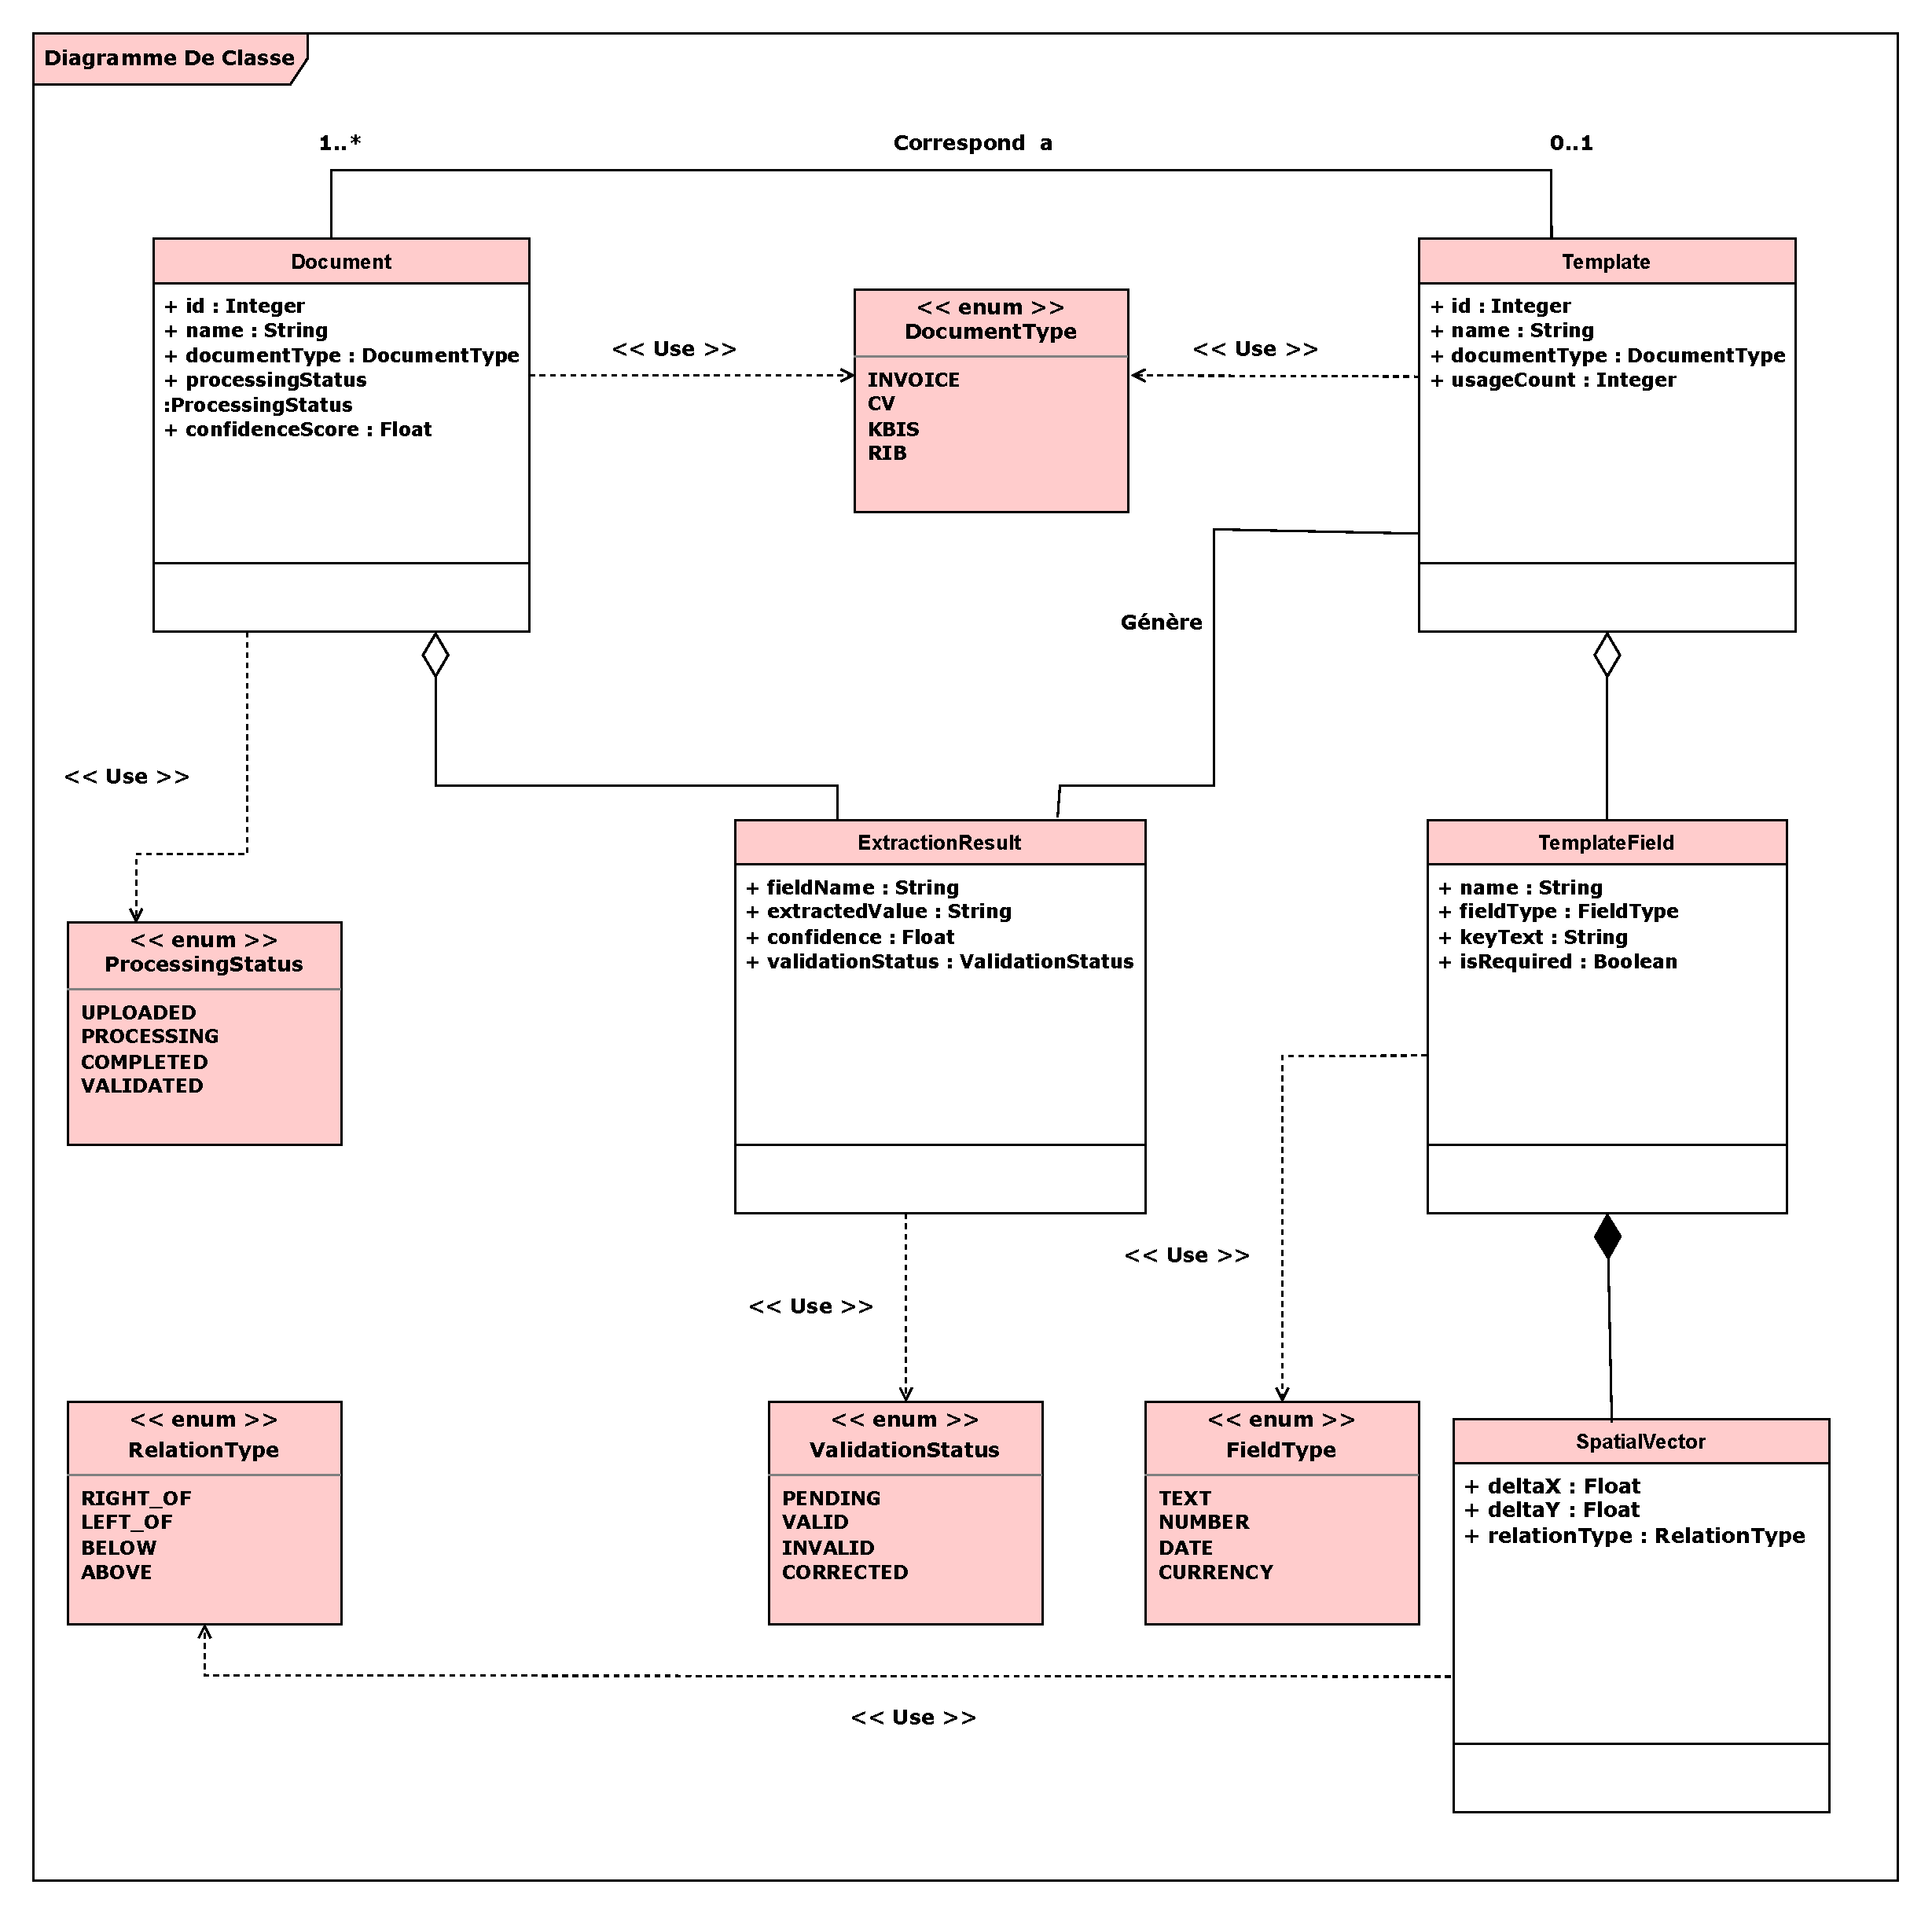
\includegraphics[width=0.9\paperwidth]{chapters/chapter04/diagrammes/DiagrammeDeClasse.pdf}}
    \caption{\itshape Diagramme de classes du module Ophélia}
    \label{fig:diagramme-classes}
\end{figure}

%==================================================================
\subsection{Diagramme de workflow général} \label{subsec:diagramme-workflow} Le \textbf{diagramme de workflow général} (figure~\ref{fig:diagramme-workflow}) rassemble en une vue unique le parcours complet d'un document, du téléversement jusqu'à l'export, en répartissant chaque activité dans le couloir de l'entité qui l'exécute : l'\textbf{Utilisateur}, le module \textbf{Ophélia}, le \textbf{Moteur OCR} et le \textbf{Moteur IA}.
 \begin{figure}[H] 
   \centering   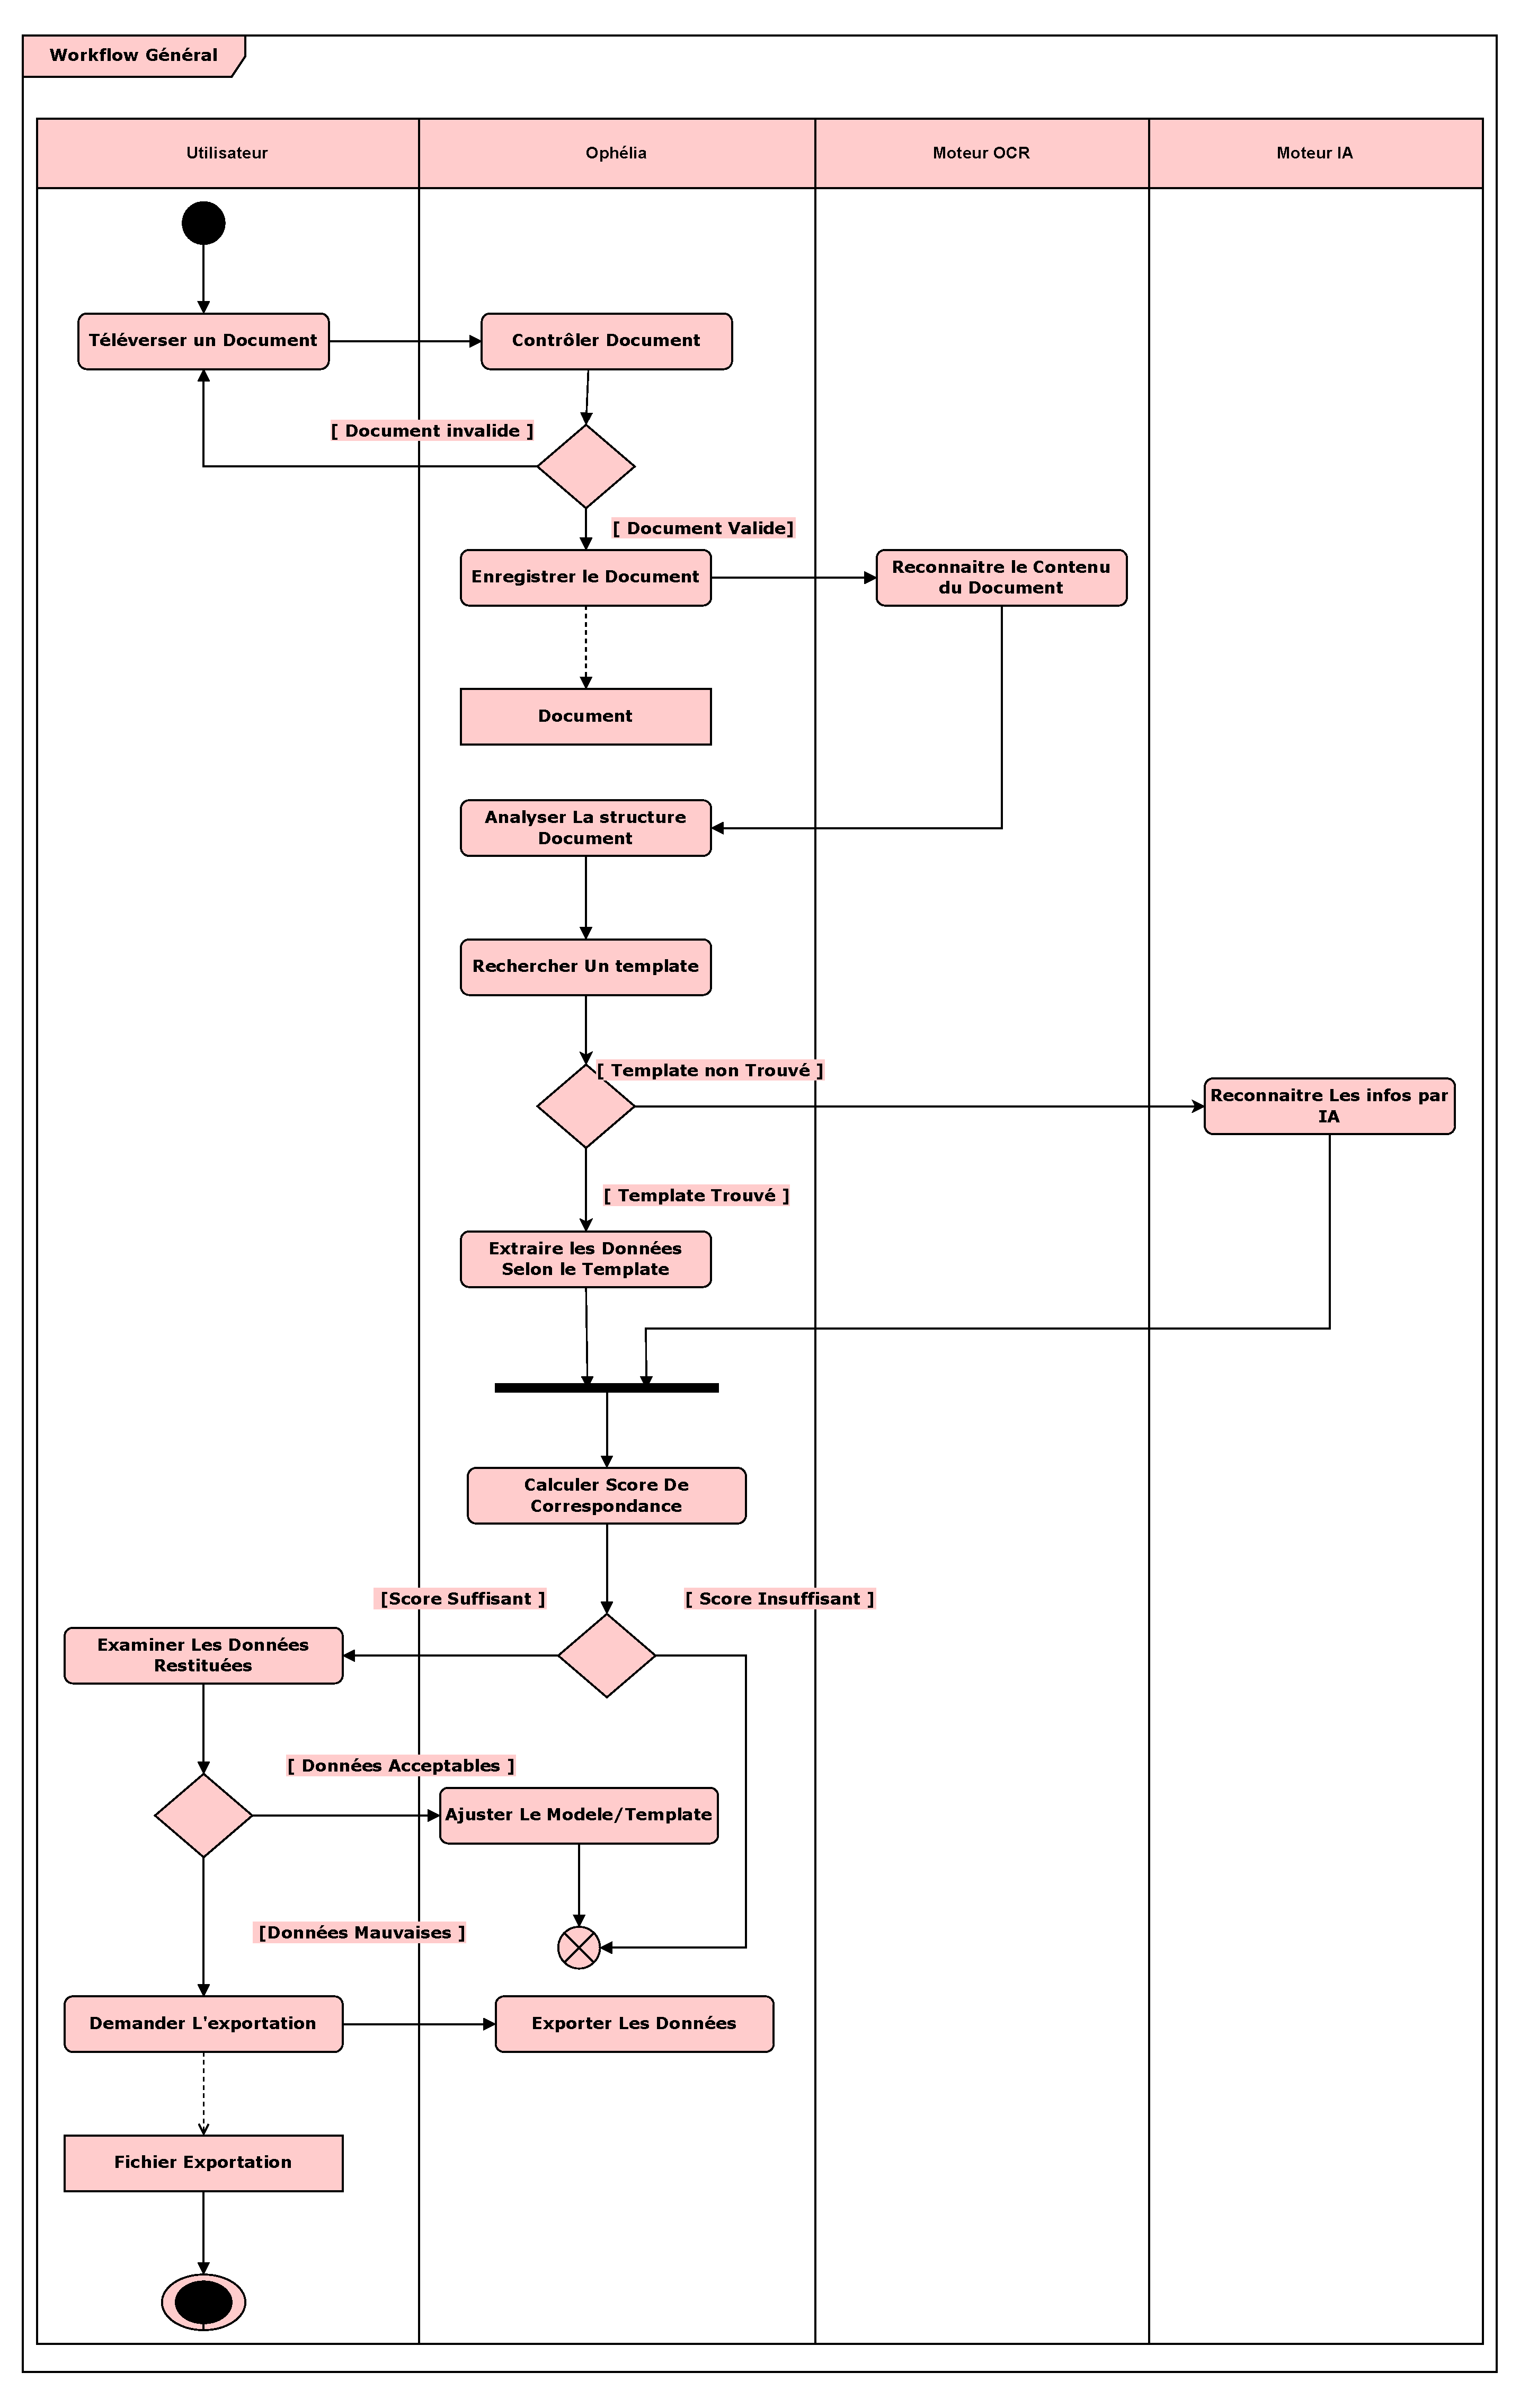
\includegraphics[height=0.9\paperwidth,keepaspectratio]{chapters/chapter04/diagrammes/DiagrammeWorkflowGeneral.pdf} \caption{\itshape Workflow général du traitement d'un document par le module Ophélia} \label{fig:diagramme-workflow}
 \end{figure} Deux branchements structurent ce parcours. Le premier matérialise la \textbf{sélection adaptative de la méthode d'extraction} : lorsqu'aucun template n'est trouvé, ou que le score de correspondance est insuffisant, le traitement bascule vers le Moteur IA. Le second impose la \textbf{validation humaine} comme passage obligé avant tout export, et renvoie les données jugées mauvaises vers l'ajustement du template, ce qui rend le module \textbf{apprenant}.

% =============================================================
%  SECTION : Diagrammes de séquence
%  À insérer dans le chapitre 4 (Méthodologie)
% =============================================================

\subsection{Diagrammes de séquence}

Les \textbf{diagrammes de séquence} modélisent les interactions entre les acteurs et les composants internes du système selon un axe temporel. Ils précisent l'\textbf{ordre chronologique des messages échangés}, les \textbf{fragments combinés} (alternatives, boucles) ainsi que la création d'objets au fil du scénario. Six cas d'utilisation critiques ont été retenus pour cette modélisation.

% ---------------------------------------------------------------
%  1. Téléverser Document
% ---------------------------------------------------------------
\subsubsection{Téléverser un document}

Ce diagramme décrit le scénario par lequel un \textbf{Utilisateur} soumet un document au système. Après sélection du fichier, \textbf{Ophélia} délègue au \textbf{Service} l'analyse du document : vérification du \textbf{format} et de la \textbf{taille}. Un fragment \textit{alt} distingue deux issues~: si le format ou la taille sont invalides, un message d'erreur est retourné à l'utilisateur~; dans le cas contraire, un objet \texttt{d:Document} est créé, puis enregistré via le \textbf{Repository} qui assure la persistance en base de données. L'utilisateur reçoit alors une confirmation de téléversement réussi.

\begin{figure}[H]
\hspace{-1cm}
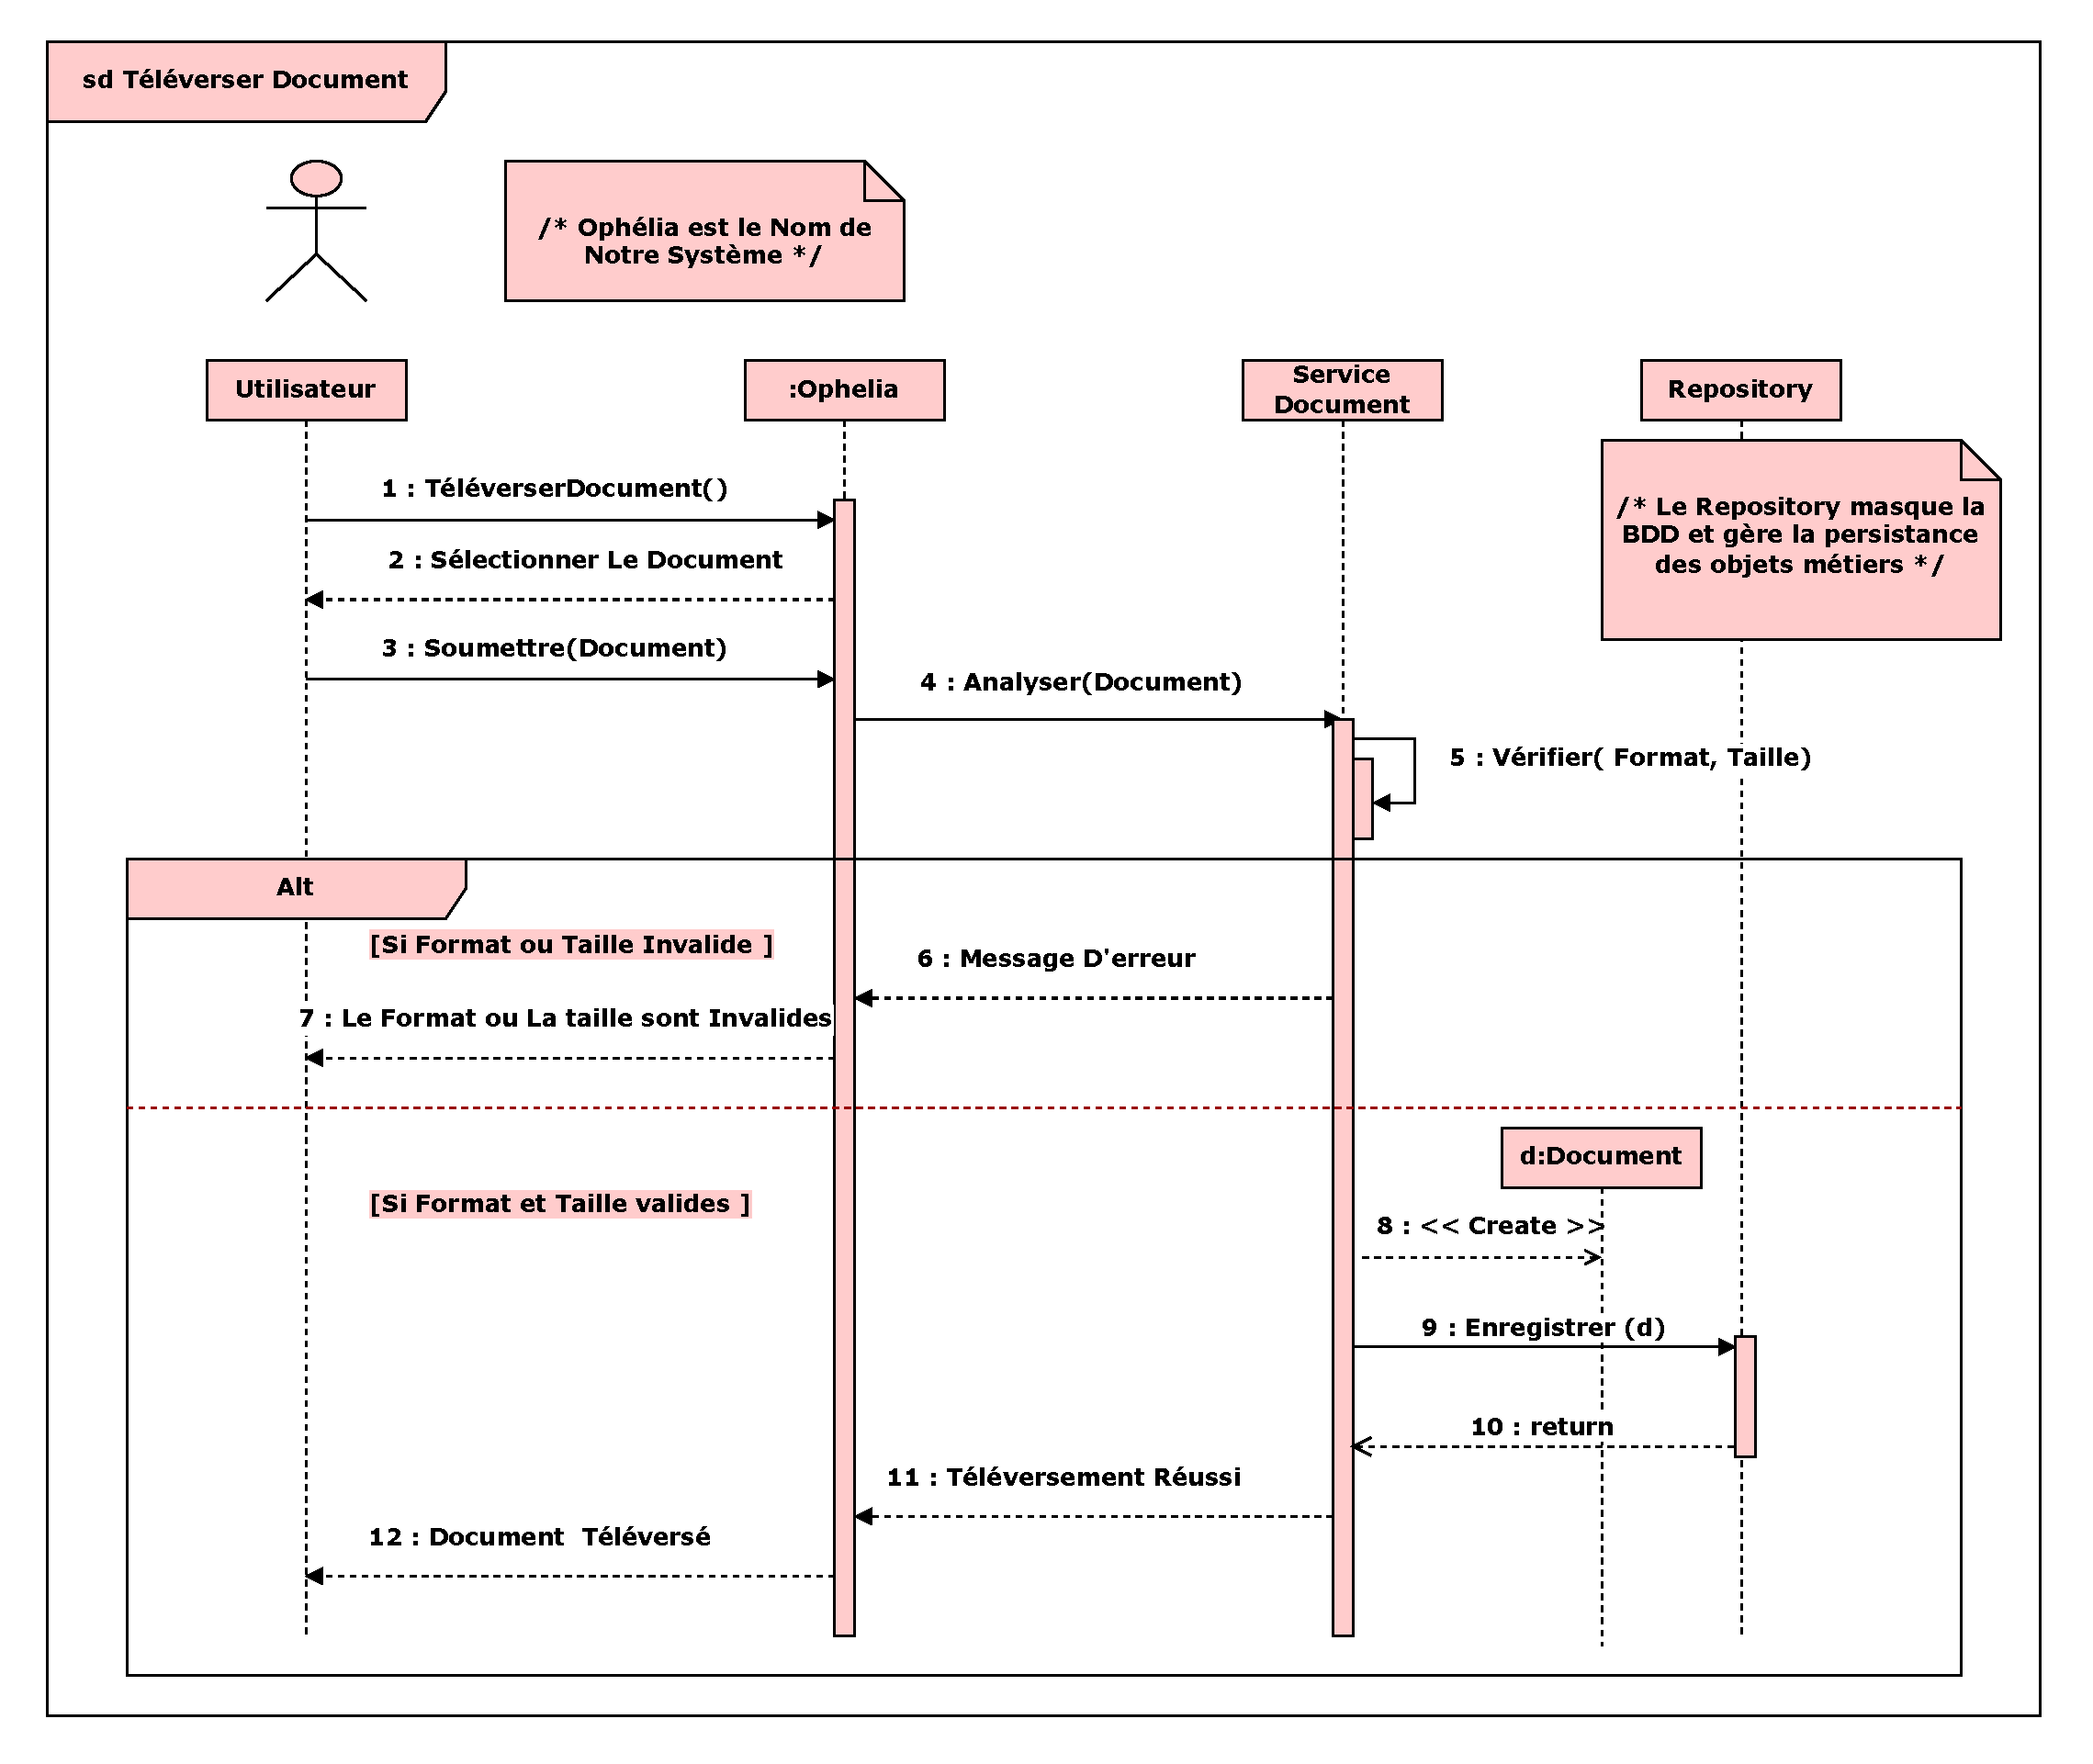
\includegraphics[width=0.9\paperwidth]{chapters/chapter04/diagrammes/DiagrammeSequenceTeleverserDocument.pdf}
\caption{ \itshape Diagramme de séquence du cas d'utilisation Téléverser un document}
\label{fig:seq-televerser-document}
\end{figure}

% ---------------------------------------------------------------
%  2. Créer Template
% ---------------------------------------------------------------
\subsubsection{Créer un template}

L'\textbf{Administrateur} initie la création d'un template en remplissant un formulaire proposé par Ophélia. Le \textbf{Service} analyse et vérifie les informations saisies. Un fragment \textit{alt} gère le cas d'informations invalides~: un message d'erreur est alors renvoyé. Si les informations ne sont pas conformes, un fragment \textit{loop} permet à l'administrateur de \textbf{corriger itérativement} chaque champ invalide jusqu'à ce que l'ensemble des données soit conforme. Une fois la validation terminée, un objet \texttt{t:Template} est créé, enregistré dans le \textbf{Repository}, et un message de confirmation est retourné.

\begin{figure}[H]
\hspace{-1cm}
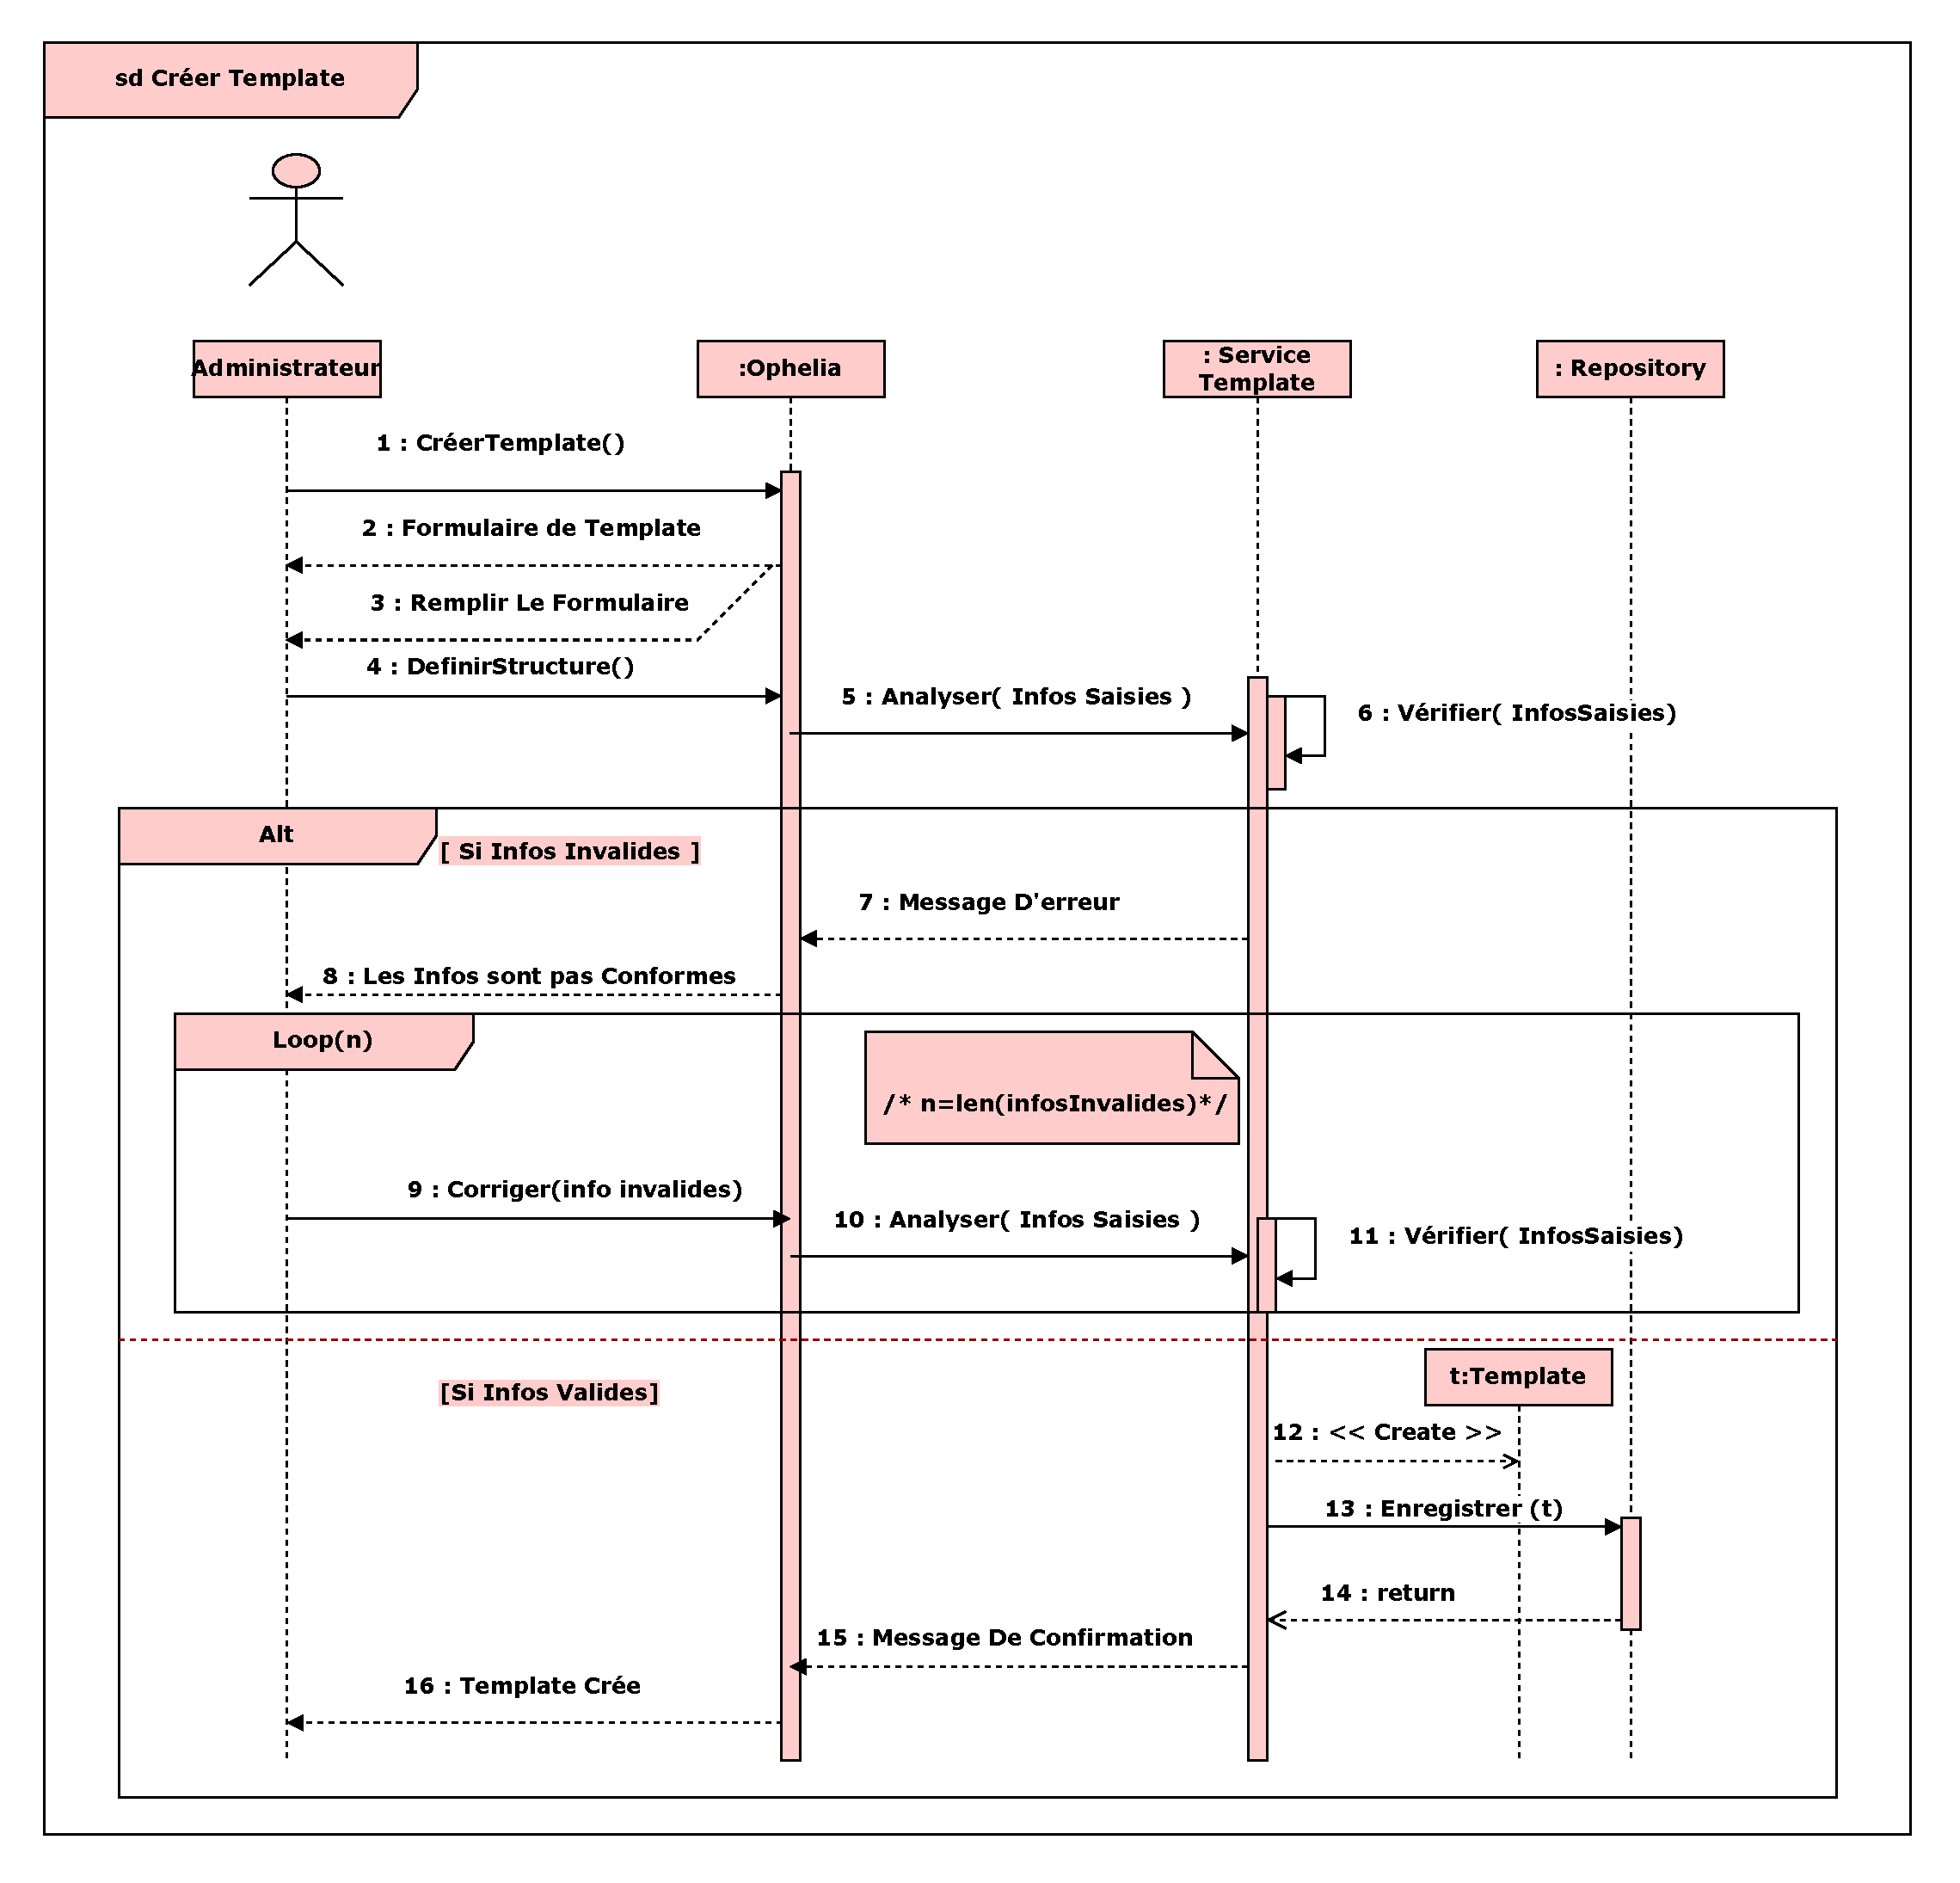
\includegraphics[width=0.9\paperwidth]{chapters/chapter04/diagrammes/DiagrammeSequenceCreerTemplate.pdf}
\caption{ \itshape Diagramme de séquence du cas d'utilisation Créer un template}
\label{fig:seq-creer-template}
\end{figure}

% ---------------------------------------------------------------
%  3. Configurer les champs d'un template
% ---------------------------------------------------------------
\subsubsection{Configurer les champs d'un template}

Ce diagramme modélise la \textbf{configuration des champs} d'un template existant. L'\textbf{Administrateur} sélectionne un template parmi la liste récupérée depuis le \textbf{Repository}. Le \textbf{Service} charge les configurations actuelles et les présente à l'administrateur, qui effectue les modifications souhaitées (ajout, lecture, modification, suppression de champs). Après soumission, un fragment \textit{alt} distingue deux cas~: si la configuration est valide, les champs sont mis à jour via le Repository et une confirmation est retournée~; si la configuration est invalide, un message d'erreur invite l'administrateur à recommencer.

\begin{figure}[H]
\hspace{-1cm}
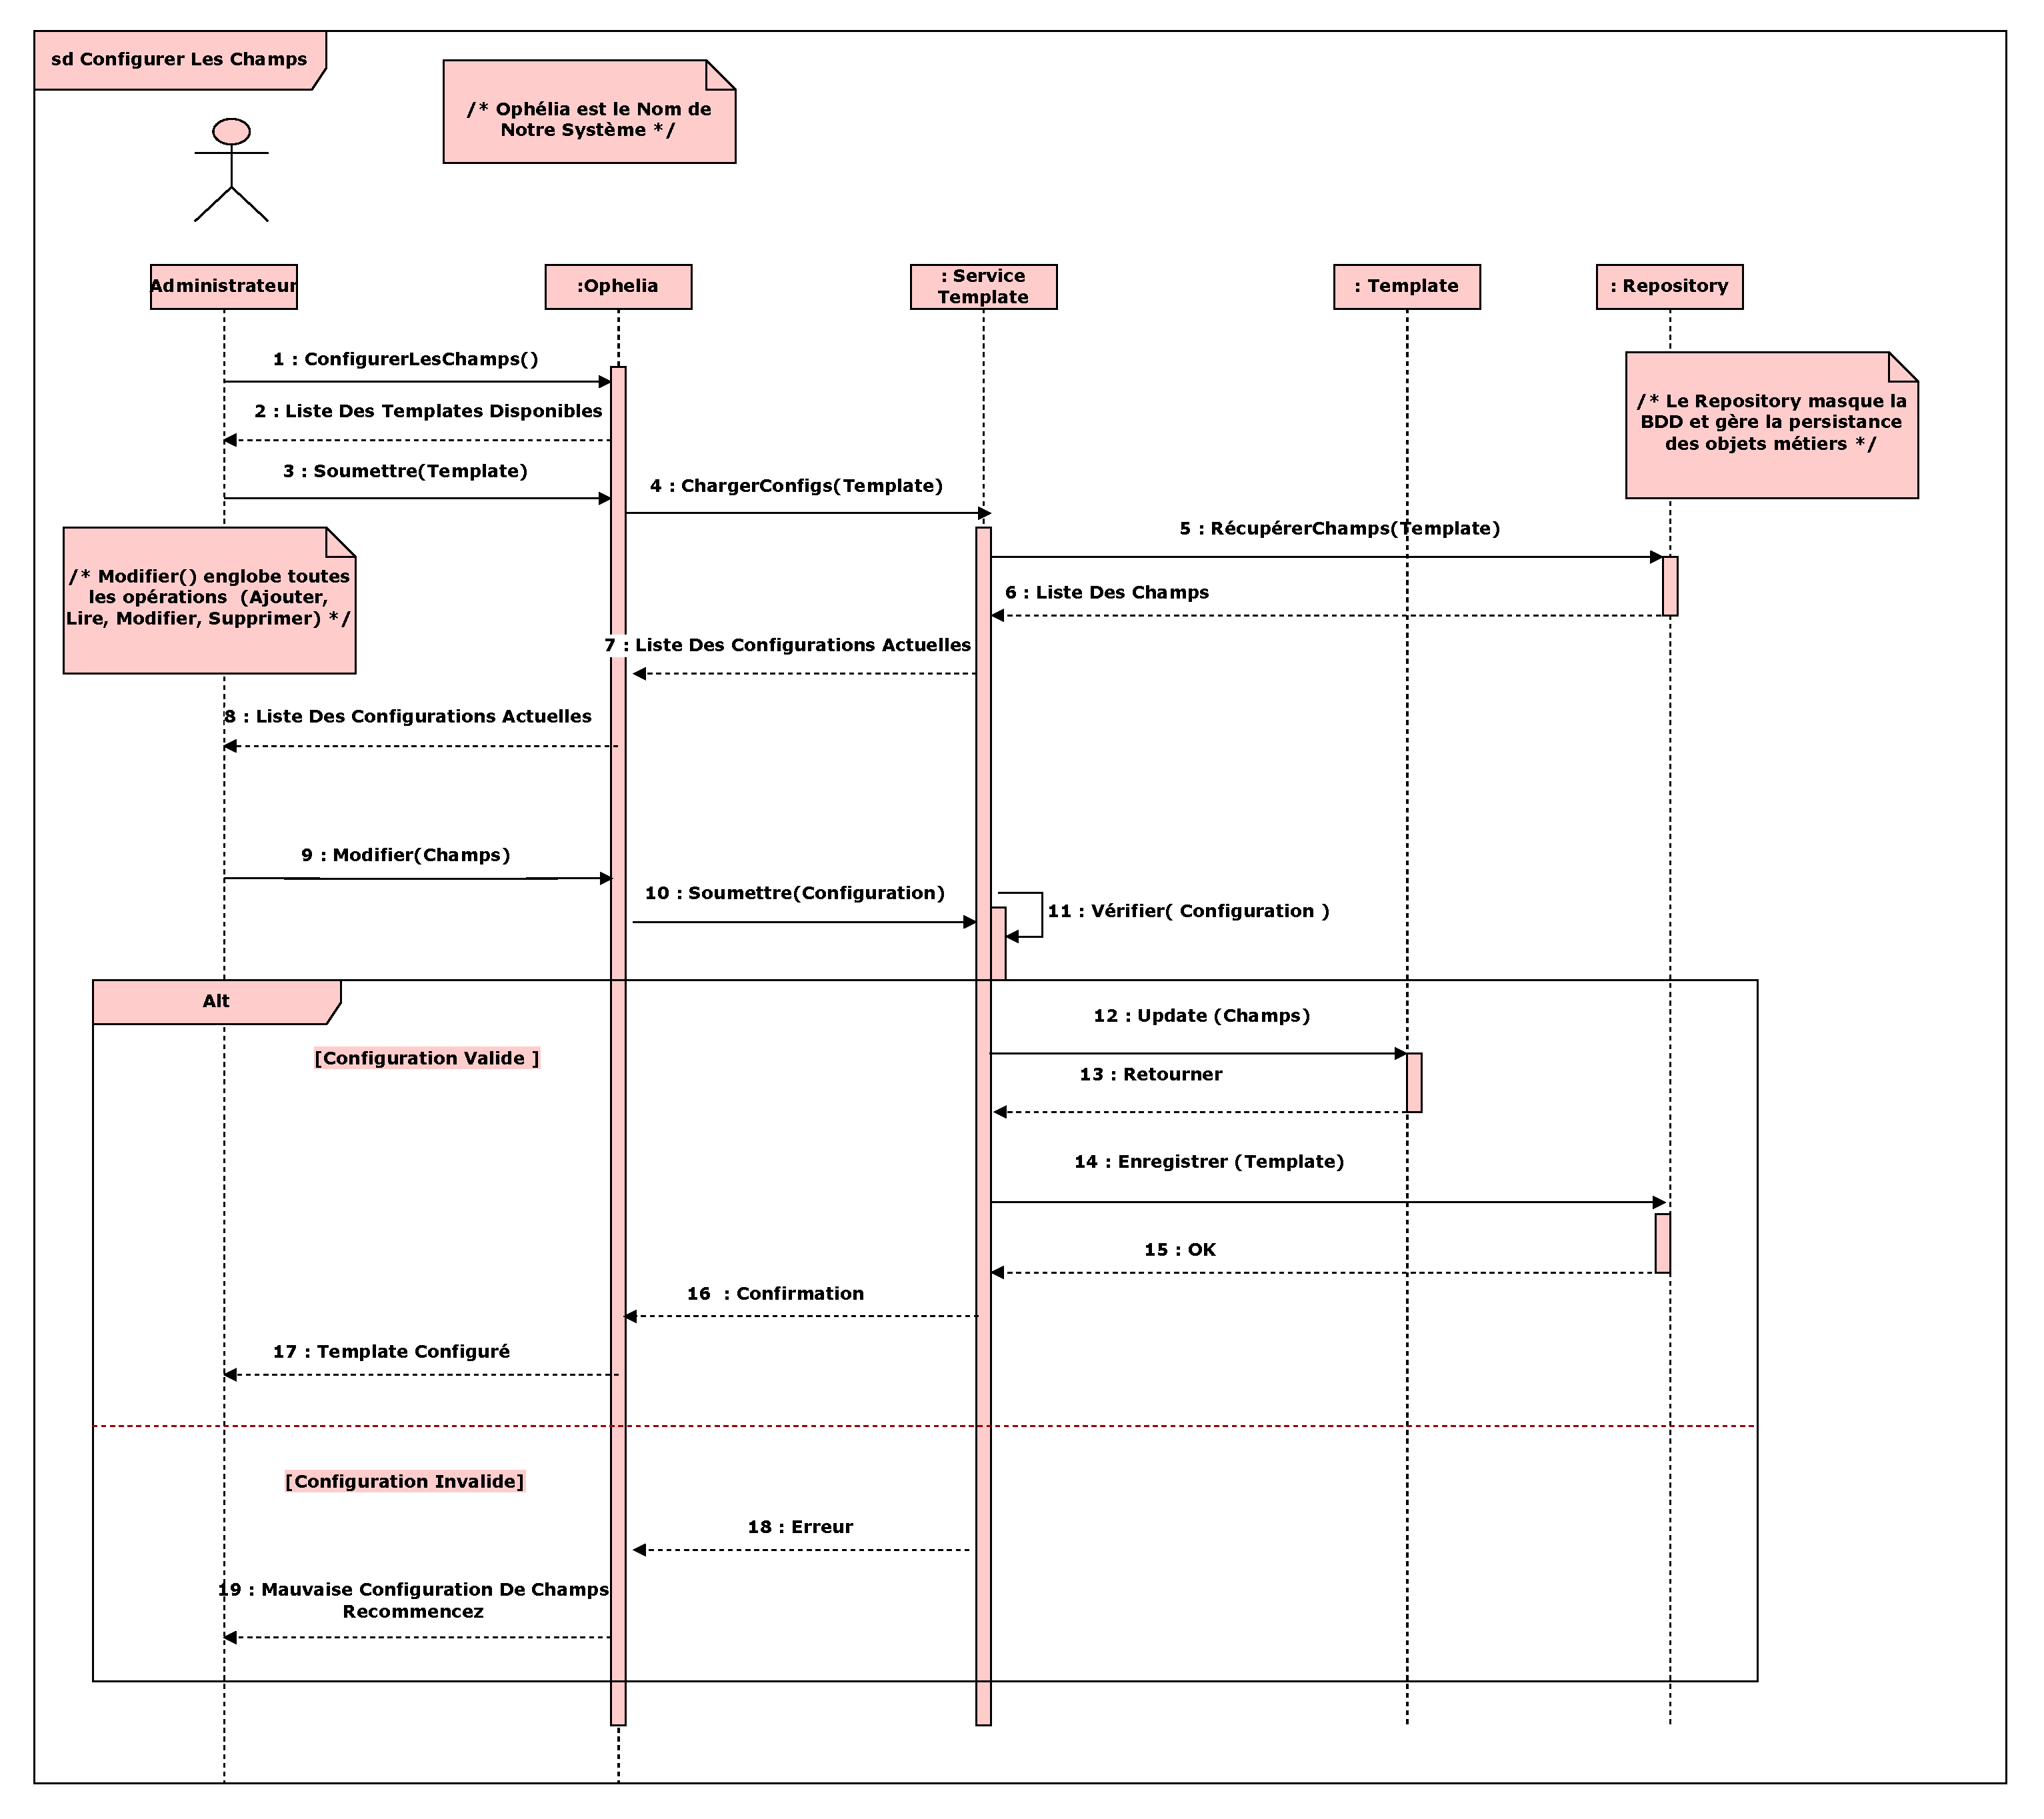
\includegraphics[width=0.9\paperwidth]{chapters/chapter04/diagrammes/DiagrammeSequenceConfigurerTemplate.pdf}
\caption{\itshape Diagramme de séquence du cas d'utilisation Configurer les champs d'un template}
\label{fig:seq-configurer-template}
\end{figure}

% ---------------------------------------------------------------
%  4. Choix de la stratégie de traitement
% ---------------------------------------------------------------
\subsubsection{Choisir la stratégie de traitement}

Ce diagramme illustre la sélection de la \textbf{stratégie de traitement} appliquée à un document soumis. Ophélia évalue d'abord les \textbf{caractéristiques du document}, puis récupère les stratégies disponibles depuis le \textbf{Repository}. Un fragment \textit{alt} distingue deux scénarios~: soit l'\textbf{Administrateur} effectue un \textbf{choix explicite} parmi les stratégies proposées, soit le système applique la \textbf{stratégie par défaut} en l'absence d'intervention. La stratégie retenue est enregistrée, le \textbf{pipeline de traitement} est configuré en conséquence, et le traitement se termine.

\begin{figure}[H]
\hspace{-1cm}
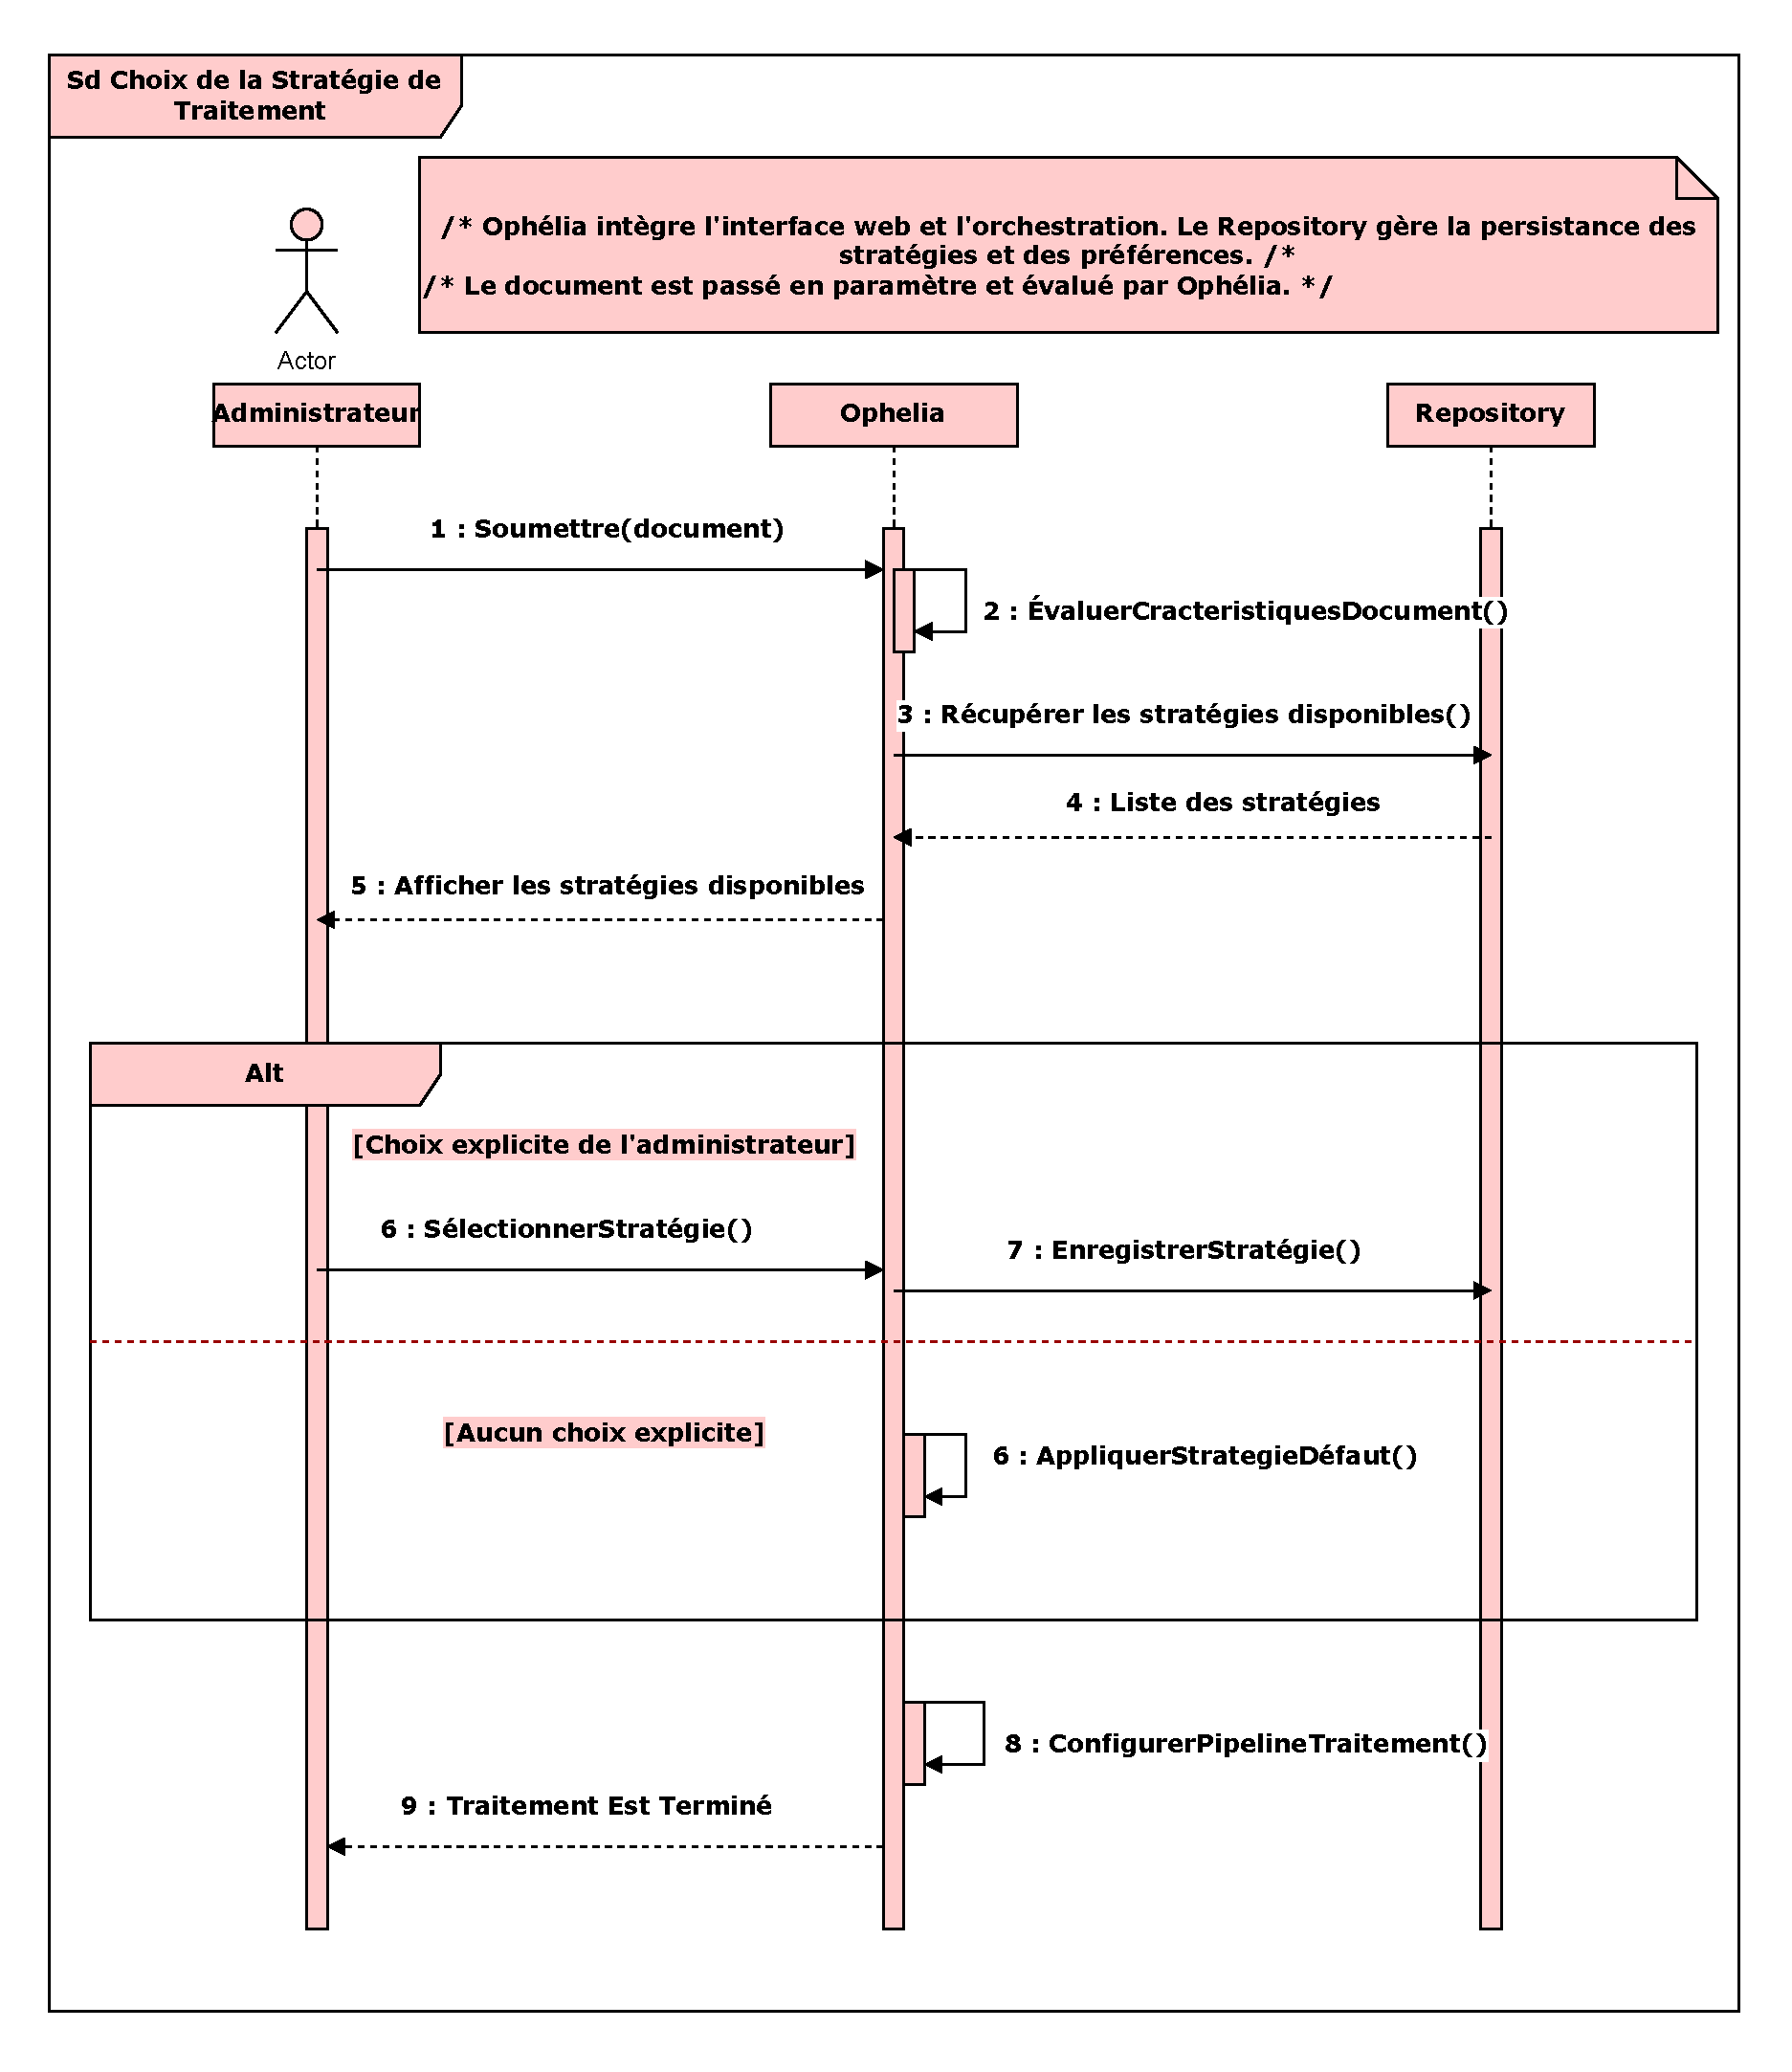
\includegraphics[width=0.9\paperwidth]{chapters/chapter04/diagrammes/DiagrammeSequenceChoixDeStrategie.pdf}
\caption{\itshape Diagramme de séquence du cas d'utilisation Choisir la stratégie de traitement}
\label{fig:seq-choix-strategie}
\end{figure}

% ---------------------------------------------------------------
%  5. Associer Document / Template (Extraction et Reconnaissance)
% ---------------------------------------------------------------
\subsubsection{Extraire et reconnaître un document}

Ce diagramme modélise le processus automatisé d'\textbf{extraction et de reconnaissance} d'un document. Le \textbf{Moteur OCR} extrait d'abord le texte brut, puis le \textbf{Service} analyse la mise en page et détecte le type de document. Un \textbf{score de correspondance} est calculé pour chaque template candidat récupéré depuis le \textbf{Repository}. Un fragment \textit{alt} distingue deux issues~: si le score est suffisant, le template retenu est \textbf{associé au document} avec son score de confiance~; dans le cas contraire, le document est marqué comme \textbf{non reconnu}, ce qui déclenche un traitement spécifique en aval.

\begin{figure}[H]
\hspace{-1cm}
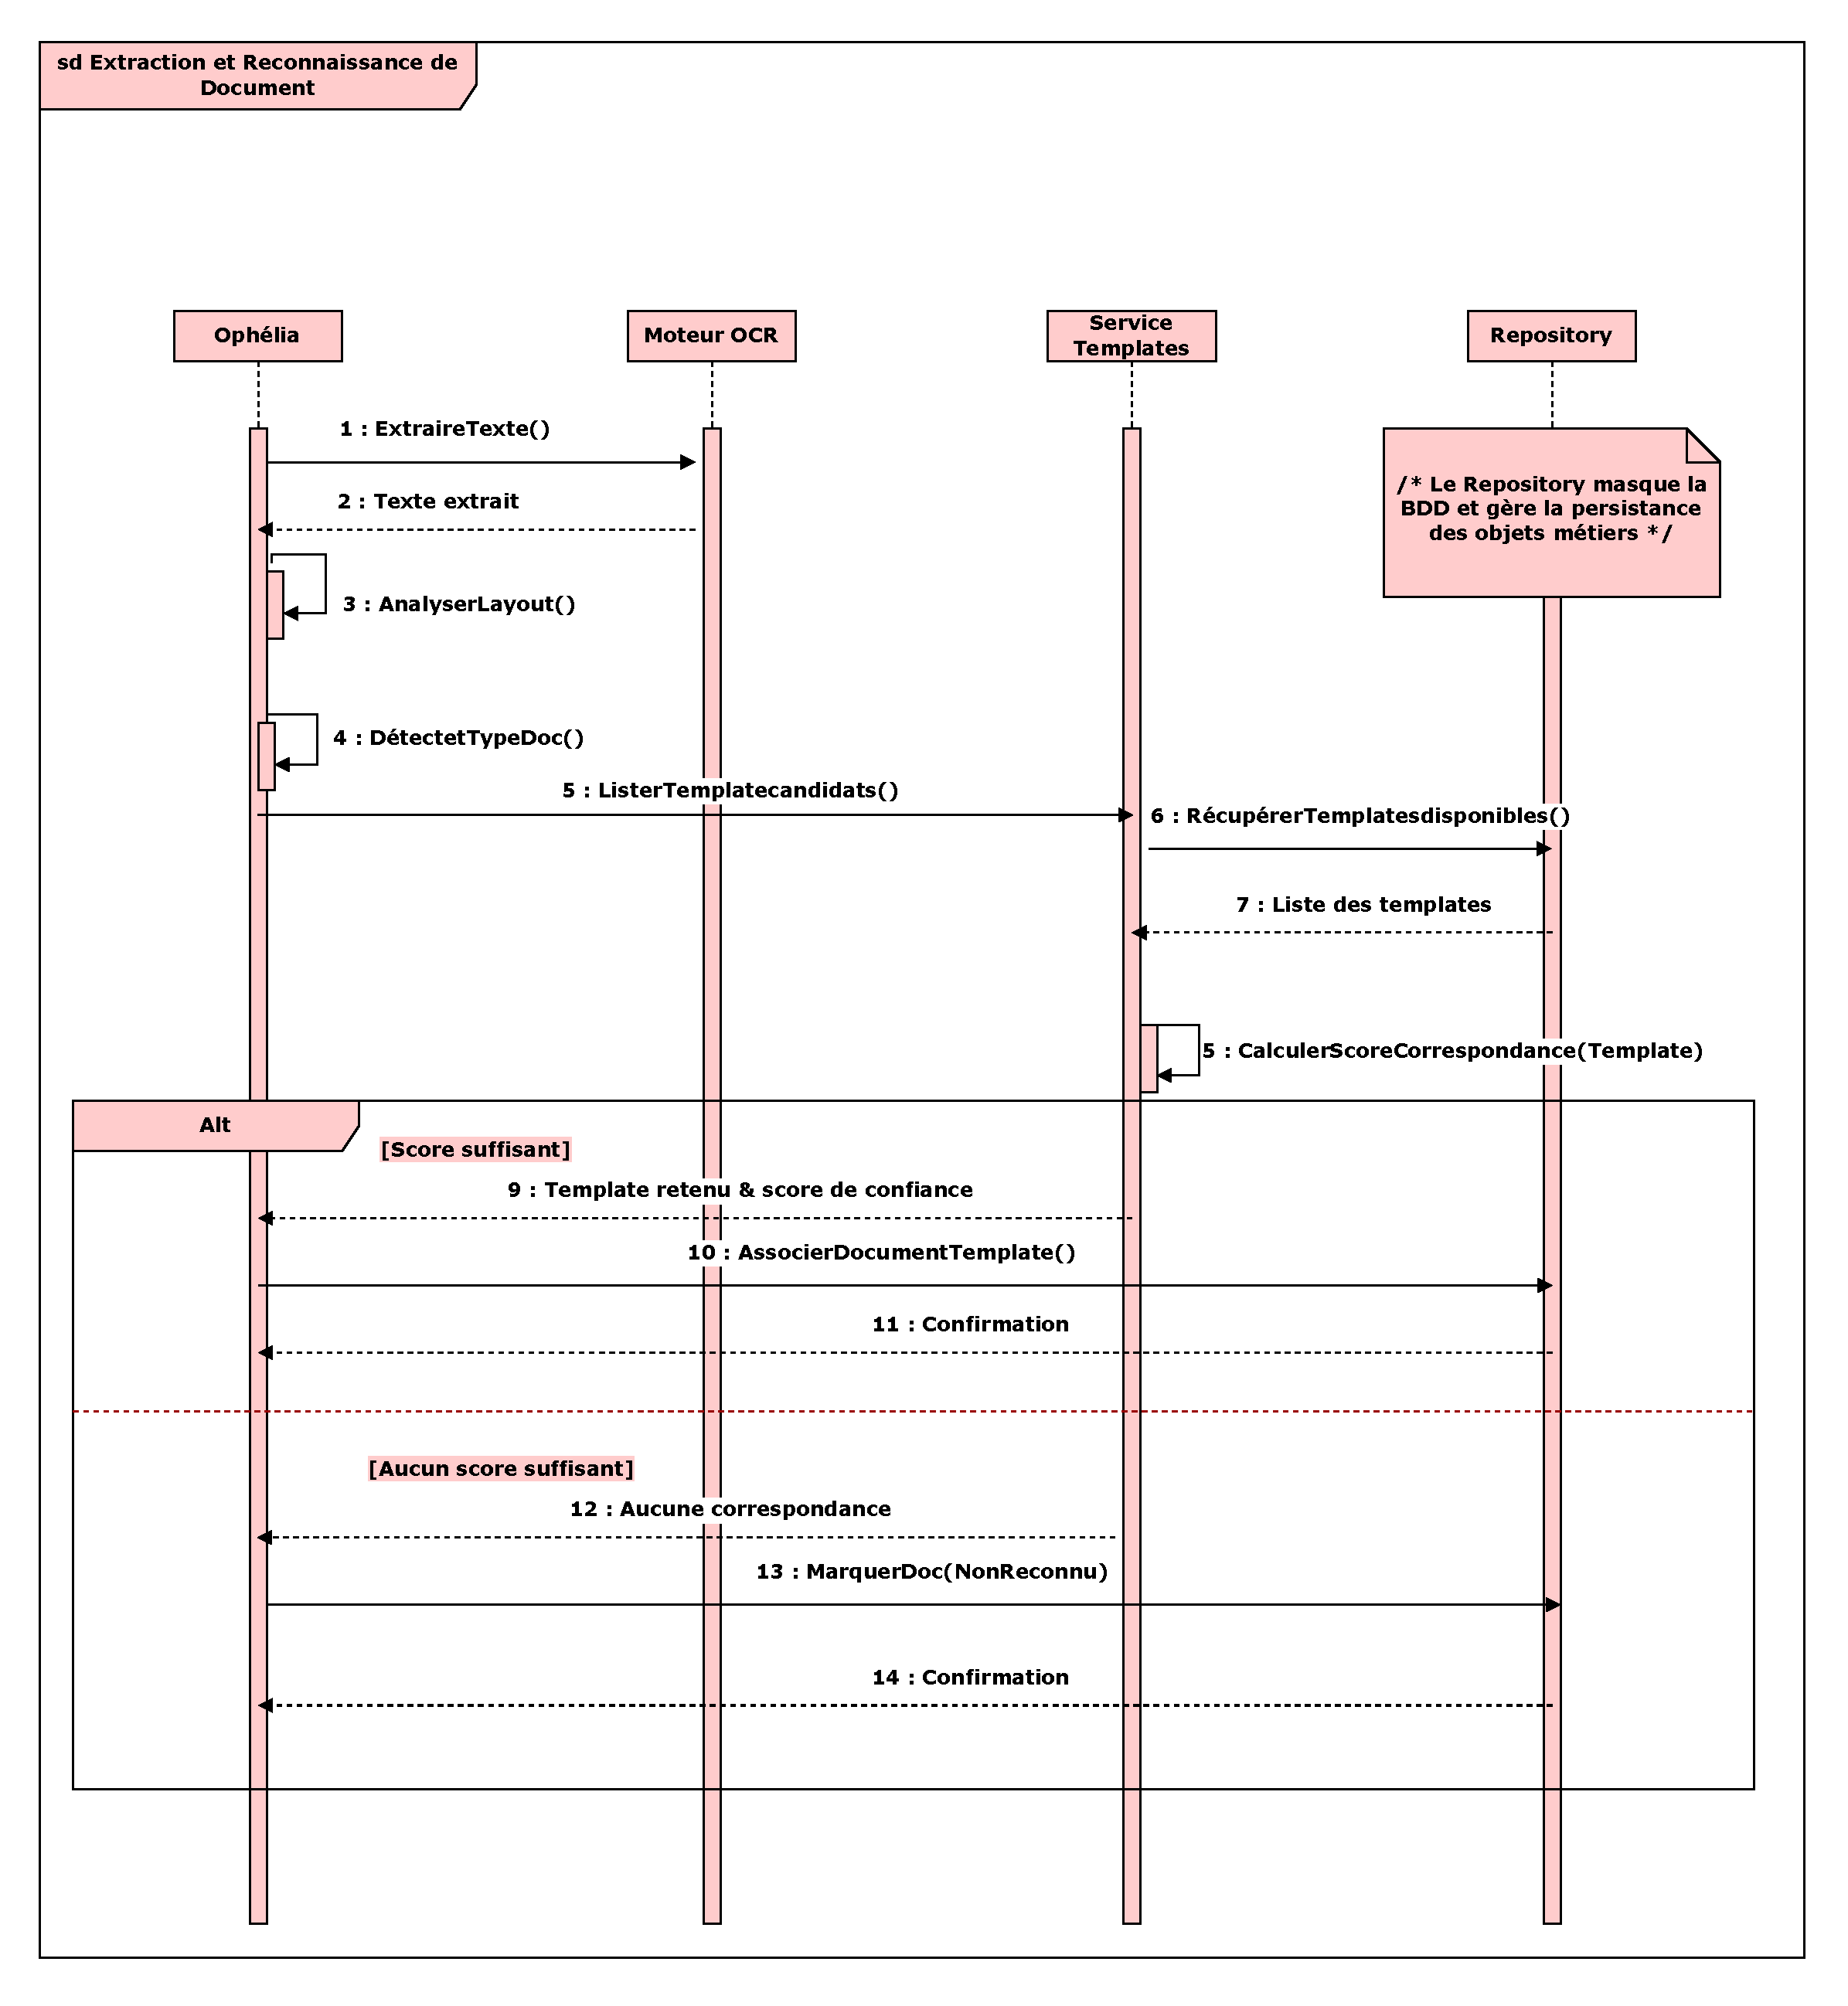
\includegraphics[width=0.9\paperwidth]{chapters/chapter04/diagrammes/DiagrammeSequenceAssocierDocumentTemplate.pdf}
\caption{\itshape Diagramme de séquence du cas d'utilisation Extraire et reconnaître un document}
\label{fig:seq-associer-document-template}
\end{figure}

% ---------------------------------------------------------------
%  6. Exporter un résultat
% ---------------------------------------------------------------
\subsubsection{Exporter un résultat}

L'\textbf{Utilisateur} sélectionne un résultat d'extraction à exporter et choisit un format parmi \textbf{XML} et \textbf{JSON}. Le \textbf{Service Export} vérifie, via le \textbf{Repository}, que le résultat a été préalablement \textbf{validé} par l'utilisateur. Un fragment \textit{alt} distingue deux cas~: si le résultat est validé, le fichier est généré dans le format choisi et mis à disposition en téléchargement~; si le résultat n'est pas encore validé, l'export est refusé et l'utilisateur est \textbf{redirigé vers l'étape de validation}.

\begin{figure}[H]
\hspace{-1cm}
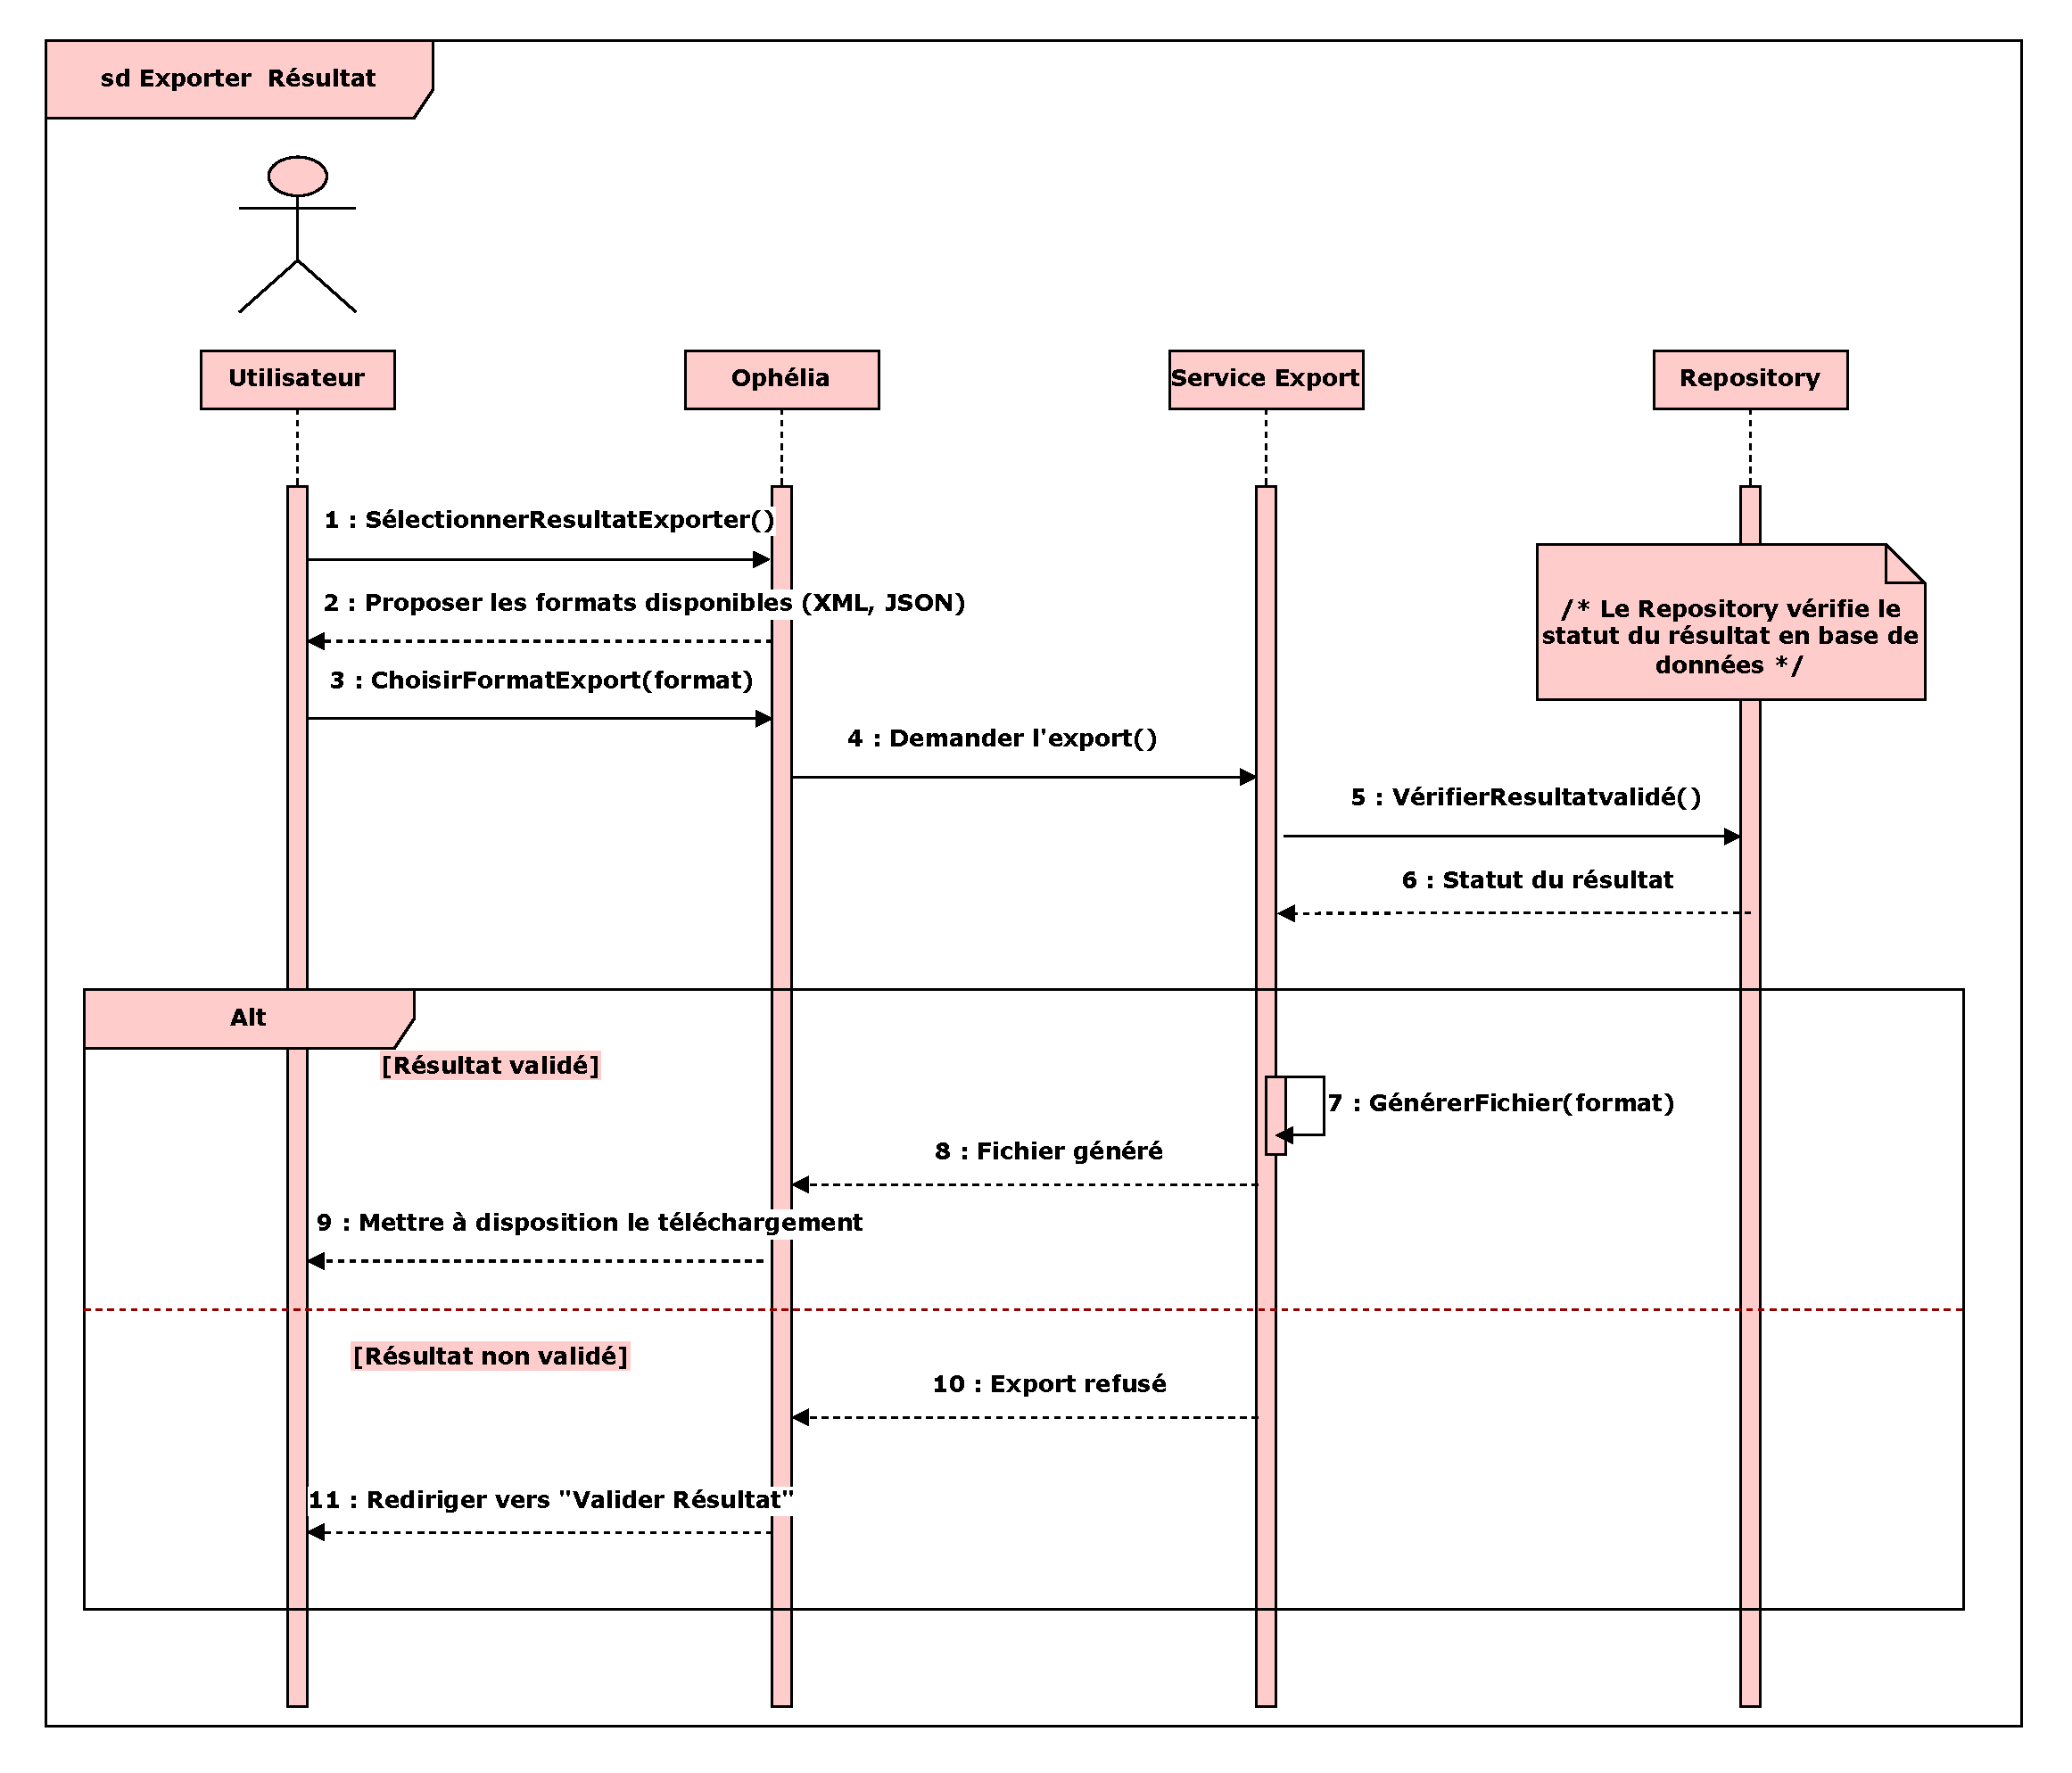
\includegraphics[width=0.9\paperwidth]{chapters/chapter04/diagrammes/DiagrammeSequenceExporterResultat.pdf}
\caption{ \itshape Diagramme de séquence du cas d'utilisation Exporter un résultat}
\label{fig:seq-exporter-resultat}
\end{figure}
%==================================================================
% Sections suivantes a completer :
% \section{Modélisation dynamique}
%     \subsection{Diagrammes d'activité}
%     \subsection{Diagrammes de séquence}
%     \subsection{Diagrammes d'états-transitions}
% \section{Conception de la solution}
%     \subsection{Architecture d'intégration dans Dolibarr}
%     \subsection{Diagramme de déploiement}
%==================================================================